% !TEX program = lualatex

\RequirePackage{silence} % :-\
    \WarningFilter{scrreprt}{Usage of package `titlesec'}
    %\WarningFilter{scrreprt}{Activating an ugly workaround}
    \WarningFilter{titlesec}{Non standard sectioning command detected}
\documentclass[ twoside,openright,titlepage,numbers=noenddot,%1headlines,
                headinclude,footinclude,cleardoublepage=empty,abstract=on,
                BCOR=5mm,paper=b5,fontsize=10pt,dvipsnames
                ]{scrbook}
\renewcommand\textsc[1]{{\fontfamily{put}\fontshape{sc}\selectfont#1}}

% use some packages
\usepackage{multicol}
\usepackage{xcolor}

%********************************************************************
% Note: Make all your adjustments in here
%*******************************************************
% !TEX program = xelatex
% ****************************************************************************************************
% classicthesis-config.tex
% formerly known as loadpackages.sty, classicthesis-ldpkg.sty, and classicthesis-preamble.sty
% Use it at the beginning of your ClassicThesis.tex, or as a LaTeX Preamble
% in your ClassicThesis.{tex,lyx} with \input{classicthesis-config}
% ****************************************************************************************************
% If you like the classicthesis, then I would appreciate a postcard.
% My address can be found in the file ClassicThesis.pdf. A collection
% of the postcards I received so far is available online at
% http://postcards.miede.de
% ****************************************************************************************************


% ****************************************************************************************************
% 0. Set the encoding of your files. UTF-8 is the only sensible encoding nowadays. If you can't read
% äöüßáéçèê∂åëæƒÏ€ then change the encoding setting in your editor, not the line below. If your editor
% does not support utf8 use another editor!
% ****************************************************************************************************
\PassOptionsToPackage{utf8}{inputenc}
  \usepackage{inputenc}

\PassOptionsToPackage{T1}{fontenc} % T2A for cyrillics
  \usepackage{fontenc}

% ****************************************************************************************************
% 1. Configure classicthesis for your needs here, e.g., remove "drafting" below
% in order to deactivate the time-stamp on the pages
% (see ClassicThesis.pdf for more information):
% ****************************************************************************************************
\usepackage[
    drafting=true,
    tocaligned=true,
    dottedtoc=true,
    eulerchapternumbers=false,
    linedheaders=false,
    palatino=true,
    beramono=true,
    floatperchapter=true,
    style=classicthesis,
    parts=true
]{classicthesis}


% ****************************************************************************************************
% 2. Personal data and user ad-hoc commands (insert your own data here)
% ****************************************************************************************************
\newcommand{\myTitle}{Animal Movement Strategies\xspace}
\newcommand{\mySubtitle}{An Homage to The Elements of Typographic Style\xspace}
\newcommand{\myDegree}{Doktor-Ingenieur (Dr.-Ing.)\xspace}
\newcommand{\myName}{Pratik Rajan Gupte\xspace}
\newcommand{\myProf}{Prof. Dr. Franz J. Weissing\xspace}
\newcommand{\myOtherProf}{Put name here\xspace}
\newcommand{\mySupervisor}{Put name here\xspace}
\newcommand{\myFaculty}{Faculty of Science and Engineering\xspace}
\newcommand{\myDepartment}{Groningen Institute for Evolutionary Life Sciences\xspace}
\newcommand{\myUni}{University of Groningen\xspace}
\newcommand{\myLocation}{Saarbrücken\xspace}
\newcommand{\myTime}{June 2018\xspace}
\newcommand{\myVersion}{\classicthesis}

% ********************************************************************
% Setup, finetuning, and useful commands
% ********************************************************************
\providecommand{\mLyX}{L\kern-.1667em\lower.25em\hbox{Y}\kern-.125emX\@}
\newcommand{\ie}{i.\,e.}
\newcommand{\Ie}{I.\,e.}
\newcommand{\eg}{e.\,g.}
\newcommand{\Eg}{E.\,g.}
% ****************************************************************************************************


% ****************************************************************************************************
% 3. Loading some handy packages
% ****************************************************************************************************
% ********************************************************************
% Packages with options that might require adjustments
% ********************************************************************
\PassOptionsToPackage{ngerman,american}{babel} % change this to your language(s), main language last
% Spanish languages need extra options in order to work with this template
%\PassOptionsToPackage{spanish,es-lcroman}{babel}
    \usepackage{babel}

\usepackage{csquotes}
\PassOptionsToPackage{%
  backend=biber,
  hyperref,
  url=false,
  isbn=false,
  doi=false,
  eprint=false,
  style=oxyear,%oxyear, % Author 1999, 2010
  dashed=true, % dashed: substitute rep. author with ---
  maxcitenames=2,
  maxbibnames=99, % default: 3, et al.
  date=year,
  uniquename=false,
  uniquelist=false,
  useprefix=true,
  sortcites=true,
  sorting=ynt, % name, year, title
  % sortfirstinits=true, % for handling names with prefixes, e.g. le Roux to be with Romano, not Leclerc.
  natbib=true % natbib compatibility mode (\citep and \citet still work)
}{biblatex}
\usepackage{biblatex}

% REMOVE THE MONTH WHICH LEADS TO EMPTY () AFTER THE ENTRY
% \AtEveryBibitem{\clearfield{pages}}
% \AtEveryBibitem{\clearfield{volume}}
\AtEveryBibitem{\clearfield{month}}
\AtEveryCitekey{\clearfield{month}}

% try to remove empty brackets
% \renewbibmacro*{issue+date}{%
%   \ifboolexpr{test {\iffieldundef{issue}} and test {\iffieldundef{year}}}
%     {}
%     {\printtext[parens]{%
%        \printfield{issue}%
%        \setunit*{\addspace}%
%        \usebibmacro{date}}%
%      \newunit}}

% % more code to remove empty brackets
% \renewbibmacro*{url+urldate}{%
%   \iffieldundef{url}
%     {}
%     {\printtext[parens]{%
%        \printfield{url}
%        \setunit{\addsemicolon\space}%
%        \printurldate}}}

\PassOptionsToPackage{fleqn}{amsmath}       % math environments and more by the AMS
  \usepackage{amsmath}

% ********************************************************************
% General useful packages
% ********************************************************************
\usepackage{graphicx} %
\usepackage{scrhack} % fix warnings when using KOMA with listings package
\usepackage{xspace} % to get the spacing after macros right
\PassOptionsToPackage{printonlyused,smaller}{acronym}
  \usepackage{acronym} % nice macros for handling all acronyms in the thesis
  %\renewcommand{\bflabel}[1]{{#1}\hfill} % fix the list of acronyms --> no longer working
  %\renewcommand*{\acsfont}[1]{\textsc{#1}}
  %\renewcommand*{\aclabelfont}[1]{\acsfont{#1}}
  %\def\bflabel#1{{#1\hfill}}
  \def\bflabel#1{{\acsfont{#1}\hfill}}
  \def\aclabelfont#1{\acsfont{#1}}
% ****************************************************************************************************
%\usepackage{pgfplots} % External TikZ/PGF support (thanks to Andreas Nautsch)
%\usetikzlibrary{external}
%\tikzexternalize[mode=list and make, prefix=ext-tikz/]
% ****************************************************************************************************


% ****************************************************************************************************
% 4. Setup floats: tables, (sub)figures, and captions
% ****************************************************************************************************
\usepackage{tabularx} % better tables
  \setlength{\extrarowheight}{3pt} % increase table row height
\newcommand{\tableheadline}[1]{\multicolumn{1}{l}{\spacedlowsmallcaps{#1}}}
\newcommand{\myfloatalign}{\centering} % to be used with each float for alignment
\usepackage{subfig}
% ****************************************************************************************************


% ****************************************************************************************************
% 5. Setup code listings
% ****************************************************************************************************
\usepackage{listings}
%\lstset{emph={trueIndex,root},emphstyle=\color{BlueViolet}}%\underbar} % for special keywords
\lstset{language=[LaTeX]Tex,%C++,
  morekeywords={PassOptionsToPackage,selectlanguage},
  keywordstyle=\color{RoyalBlue},%\bfseries,
  basicstyle=\small\ttfamily,
  %identifierstyle=\color{NavyBlue},
  commentstyle=\color{Green}\ttfamily,
  stringstyle=\rmfamily,
  numbers=none,%left,%
  numberstyle=\scriptsize,%\tiny
  stepnumber=5,
  numbersep=8pt,
  showstringspaces=false,
  breaklines=true,
  %frameround=ftff,
  %frame=single,
  belowcaptionskip=.75\baselineskip
  %frame=L
}

\lstdefinestyle{customR}{
  belowcaptionskip=1\baselineskip,
  captionpos=b,
  breaklines=true,
%   numbers=left,
  frame=L,
  xleftmargin=\parindent,
  language=R,
  showstringspaces=false,
  basicstyle=\small\ttfamily\color{black},
  keywordstyle=\ttfamily,
  commentstyle=\color{commentstyleCol},   % comment style
  stringstyle=\color{stringstyleCol}      % string literal style
}
% ****************************************************************************************************




% ****************************************************************************************************
% 6. Last calls before the bar closes
% ****************************************************************************************************
% ********************************************************************
% Her Majesty herself
% ********************************************************************
\usepackage{classicthesis}

% ********************************************************************
% Fine-tune hyperreferences (hyperref should be called last)
% ********************************************************************
\hypersetup{%
  %draft, % hyperref's draft mode, for printing see below
  colorlinks=true, linktocpage=true, pdfstartpage=3, pdfstartview=FitV,%
  % uncomment the following line if you want to have black links (e.g., for printing)
  %colorlinks=false, linktocpage=false, pdfstartpage=3, pdfstartview=FitV, pdfborder={0 0 0},%
  breaklinks=true, pageanchor=true,%
  pdfpagemode=UseNone, %
  % pdfpagemode=UseOutlines,%
  plainpages=false, bookmarksnumbered, bookmarksopen=true, bookmarksopenlevel=1,%
  hypertexnames=true, pdfhighlight=/O,%nesting=true,%frenchlinks,%
  urlcolor=CTurl, 
  linkcolor=, 
  citecolor=black, %pagecolor=RoyalBlue,%
  %urlcolor=Black, linkcolor=Black, citecolor=Black, %pagecolor=Black,%
  pdftitle={\myTitle},%
  pdfauthor={\textcopyright\ \myName, \myUni, \myFaculty},%
  pdfsubject={},%
  pdfkeywords={},%
  pdfcreator={pdfLaTeX},%
  pdfproducer={LaTeX with hyperref and classicthesis}%
}


% ********************************************************************
% Setup autoreferences (hyperref and babel)
% ********************************************************************
% There are some issues regarding autorefnames
% http://www.tex.ac.uk/cgi-bin/texfaq2html?label=latexwords
% you have to redefine the macros for the
% language you use, e.g., american, ngerman
% (as chosen when loading babel/AtBeginDocument)
% ********************************************************************
\makeatletter
\@ifpackageloaded{babel}%
  {%
    \addto\extrasamerican{%
      \renewcommand*{\figureautorefname}{Figure}%
      \renewcommand*{\tableautorefname}{Table}%
      \renewcommand*{\partautorefname}{Part}%
      \renewcommand*{\chapterautorefname}{Chapter}%
      \renewcommand*{\sectionautorefname}{Section}%
      \renewcommand*{\subsectionautorefname}{Section}%
      \renewcommand*{\subsubsectionautorefname}{Section}%
    }%
    \addto\extrasngerman{%
      \renewcommand*{\paragraphautorefname}{Absatz}%
      \renewcommand*{\subparagraphautorefname}{Unterabsatz}%
      \renewcommand*{\footnoteautorefname}{Fu\"snote}%
      \renewcommand*{\FancyVerbLineautorefname}{Zeile}%
      \renewcommand*{\theoremautorefname}{Theorem}%
      \renewcommand*{\appendixautorefname}{Anhang}%
      \renewcommand*{\equationautorefname}{Gleichung}%
      \renewcommand*{\itemautorefname}{Punkt}%
    }%
      % Fix to getting autorefs for subfigures right (thanks to Belinda Vogt for changing the definition)
      \providecommand{\subfigureautorefname}{\figureautorefname}%
    }{\relax}
\makeatother


% ********************************************************************
% Development Stuff
% ********************************************************************
\listfiles
%\PassOptionsToPackage{l2tabu,orthodox,abort}{nag}
%  \usepackage{nag}
%\PassOptionsToPackage{warning, all}{onlyamsmath}
%  \usepackage{onlyamsmath}


% ****************************************************************************************************
% 7. Further adjustments (experimental)
% ****************************************************************************************************

%\DeclareRobustCommand{\spacedallcaps}[1]{\color{Black} \textls[90]{\bfseries\scshape\large{\MakeTextUppercase{#1}}} \par}

%\DeclareRobustCommand{\maintitle}[1]{{\fontsize{70}{50}\selectfont {\scshape{#1}}\par}}
      
%\DeclareRobustCommand{\spacedlowsmallcaps}[1]{\textls[80]{{#1}}}

%\DeclareRobustCommand{\tocchapter}[1]{{{#1}}}
%\DeclareRobustCommand{\tocpart}[1]{{\bfseries\large{#1}}}

% ********************************************************************
% Changing the text area
% ********************************************************************
%\areaset[current]{312pt}{761pt} % 686 (factor 2.2) + 33 head + 42 head \the\footskip
%\setlength{\marginparwidth}{7em}%
%\setlength{\marginparsep}{2em}%

% ********************************************************************
% Using different fonts
% ********************************************************************
%\usepackage[oldstylenums]{kpfonts} % oldstyle notextcomp
%\usepackage[osf]{libertine}
%\usepackage{libertine}
%\usepackage{fonts}
%\usepackage[T1]{fontenc}
%\usepackage[usefilenames,RMstyle=Light,SSstyle=Light,TTstyle=Light,DefaultFeatures={Ligatures=Common}]{plex-otf}
%\usepackage[light,condensed,math]{iwona}
%\renewcommand{\sfdefault}{iwona}
%\usepackage{lmodern} % <-- no osf support :-(
%\usepackage{cfr-lm} %
%\usepackage[urw-garamond]{mathdesign} <-- no osf support :-(
%\usepackage[default,osfigures]{opensans} % scale=0.95
%\usepackage[sfdefault]{FiraSans}
% \usepackage[opticals,mathlf]{MinionPro} % onlytext
% ********************************************************************
%\usepackage[largesc,osf]{newpxtext}
%\linespread{1.05} % a bit more for Palatino
% Used to fix these:
% https://bitbucket.org/amiede/classicthesis/issues/139/italics-in-pallatino-capitals-chapter
% https://bitbucket.org/amiede/classicthesis/issues/45/problema-testatine-su-classicthesis-style
% ********************************************************************
% ****************************************************************************************************


%********************************************************************
% Bibliographies
%*******************************************************
% \RequirePackage[authoryear,sort]{natbib}

% \usepackage{citation-style-language}
% \cslsetup{style = apa}
\addbibresource{chapters/preprocessing.bib}
\addbibresource{chapters/kleptomove.bib}
% \addbibresource{Bibliography.bib}
% \addbibresource[label=ownpubs]{AMiede_Publications.bib}

%********************************************************************
% Hyphenation
%*******************************************************
%\hyphenation{put special hyphenation here}

%\usepackage{sourcesanspro}   % scaling is recommended
\usepackage{fontspec}
% \usepackage[xcharter]{newtxmath}
% \setmainfont{Vollkorn}[
%   Scale=0.9274,% to match the math fonts
%   Extension=.otf,
%   UprightFont=*-Regular,
%   ItalicFont=*-Italic,
%   BoldFont=*-Bold,
%   BoldItalicFont=*-BoldItalic,
% ]
% \setmainfont{Source Serif Pro}
% \setmainfont{Libre Baskerville}
% \usepackage[usefilenames,RMstyle={Text,Semibold},SSstyle={Text,Semibold},TTstyle={Text,Semibold},DefaultFeatures={Ligatures=Common}]{plex-otf}
\setmainfont{XCharter}
\setmathfont{Erewhon Math}
\setsansfont{Oswald}[Extension = .ttf, UprightFont = *-Light,BoldFont = *-Regular]
% \setsansfont{Libre Franklin}
% \setmathfont{TeX Gyre Schola Math}
% \usepackage{unicode-math}
% \setmathfont{XCharter}
% \newfontfamily\mysans{Source Sans Pro}

\renewcommand*{\bibfont}{\footnotesize}

\usepackage{setspace}

\setlength{\parindent}{1.5em}
% \setlength{\parskip}{0.5em}

\renewcommand{\chapterNumber}{%
  \color{Black}\fontsize{60}{60} \bfseries}\par

\usepackage{enumitem}
\setlist[description]{leftmargin=\parindent,labelindent=\parindent}

\makeatletter
% fix part heading format
\titleformat{\part}[display]
        {\ct@altfont\centering\LARGE\sffamily}%
        {\thispagestyle{empty}\scshape\sffamily\partname~\MakeTextUppercase{\thepart}}{1em}%
        {\color{Gray}\scshape\bfseries\huge\sffamily}[\bigskip\normalfont\normalsize\color{Black}\begin{quote}\ctparttext@print\end{quote}]
        
% fix chapter heading format
\titleformat{\chapter}[display]%
    % \setbox0=\hbox{\chapterNumber\thechapter\hspace{10pt}\vline\ }%
    {\relax}{\mbox{}\oldmarginpar{\chapterNumber\sffamily\thechapter}}{0pt}%
    {\raggedright\huge\sffamily\bfseries}[\normalsize\vspace*{.8\baselineskip}\titlerule]%

% fix section format
\titleformat{\section}
    {\relax}{\thesection}{1em}{\large\sffamily\bfseries}

% fix section format
\titleformat{\subsection}
    {\relax}{\thesubsection}{1em}{\large\sffamily}

% fix section format
\titleformat{\paragraph}
    {\relax}{\theparagraph}{1em}{\sffamily}

% \usepackage[left]{lineno}

% parts in toc
\renewcommand{\cftpartfont}{\scshape\sffamily}%
% chapters in toc
\renewcommand{\cftchappresnum}{\sffamily}%
\renewcommand{\cftchapaftersnumb}{\sffamily}%
\renewcommand{\cftchapfont}{\sffamily}%
\renewcommand{\cftchappagefont}{\sffamily}%

% for stylistic elements
\usepackage{lettrine}
%% Dropped capital for first letter of main text
\newcommand{\dropcap}[1]{\lettrine[lines=2,lraise=0.05,findent=0.1em, nindent=0em]{{\bfseries\rmfamily{#1}}}{}}
\usepackage{adforn}

\makeatother

\DeclareCaptionFont{quack}{\mysans}
\usepackage{caption}
\setcapindent{0pt}

\captionsetup{
  font={footnotesize},
  labelfont=bf,
  justification=justified,
  format=plain
}

% paragraph spacing
% \setlength{\parskip}{1em}

% ********************************************************************
% GO!GO!GO! MOVE IT!
%*******************************************************
\begin{document}

\raggedright
\frenchspacing
\raggedbottom
\setlength{\parindent}{2em}
\selectlanguage{american} % american ngerman
%\renewcommand*{\bibname}{new name}
%\setbibpreamble{}
% \pagenumbering{roman}
\pagestyle{plain}
%********************************************************************
% Frontmatter
%*******************************************************
% %*******************************************************
% Little Dirty Titlepage
%*******************************************************
\thispagestyle{empty}
%\pdfbookmark[1]{Titel}{title}
%*******************************************************
\begin{center}
    \spacedlowsmallcaps{\myName} \\ \medskip

    \begingroup
        \color{CTtitle}\spacedallcaps{\myTitle}
    \endgroup
\end{center}

%*******************************************************
% Cover Titlepage
%*******************************************************
\definecolor{myOrange}{rgb}{0.969,0.965,0.945}

\begin{titlepage}
    \pagecolor{myOrange}\afterpage{\nopagecolor}
    %\pdfbookmark[1]{\myTitle}{titlepage}
    % if you want the titlepage to be centered, uncomment and fine-tune the line below (KOMA classes environment)
    \begin{addmargin}[-1cm]{-3cm}
    % \begin{center}
        \linespread{1.5}
        % \large

        \hfill

        % \vfill
        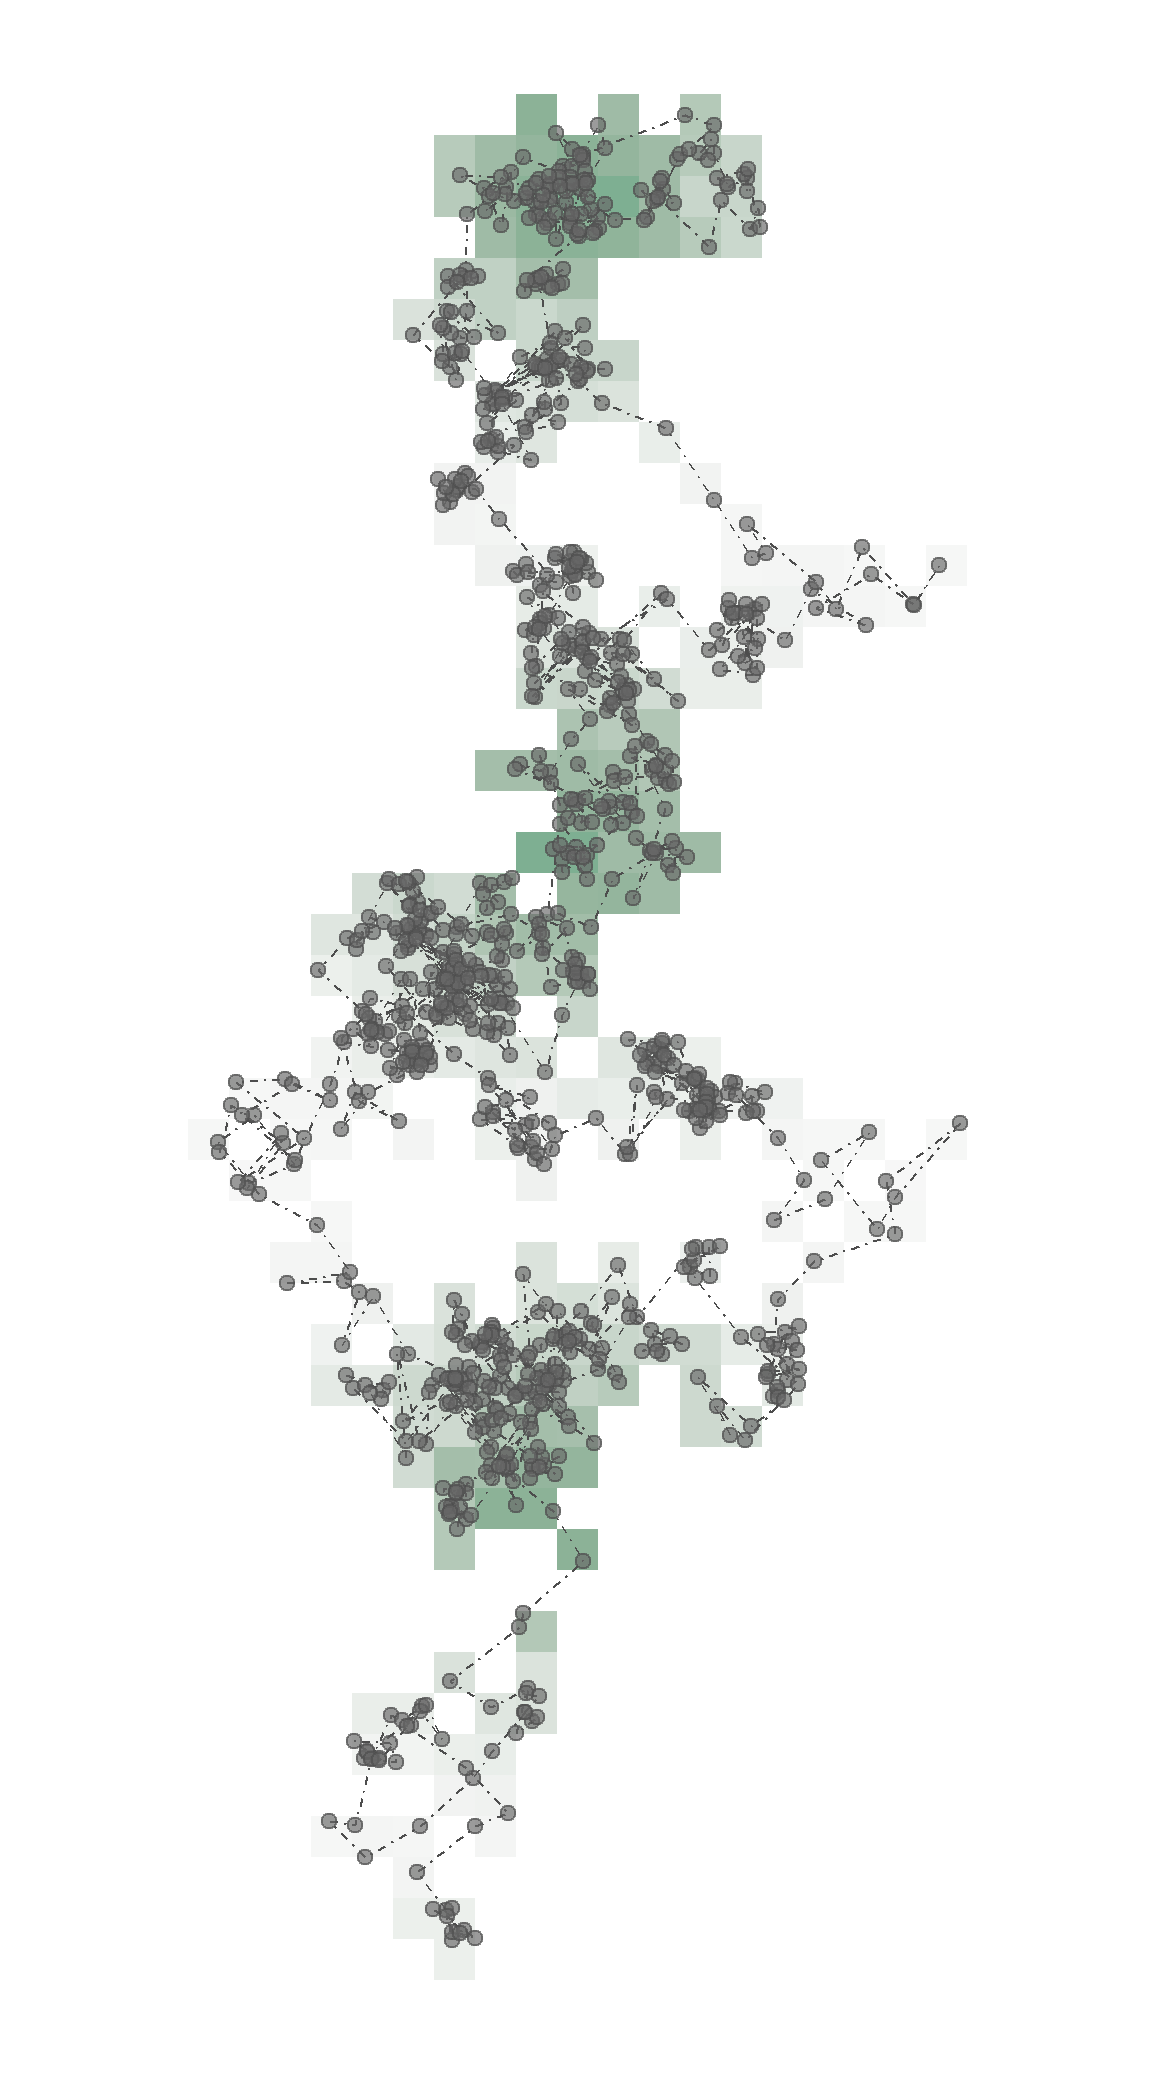
\includegraphics[width=1.0\textwidth,
          align=h,
          smash=br,
          hsmash=r,
          hshift=0.5\textwidth,
          % vshift=1cm,     % adjust the vertical position
          % hshift=-1.5cm
          ]{figures/cover_2.png}
        {
          \begin{flushleft}
            \color{SteelBlue4}{\fontsize{60}{50} \bfseries\sffamily{ANIMAL\\MOVEMENT\\STRATEGIES}\par}\par
          \end{flushleft}
        }
        % \makebox[0pt][h]{%
          % \raisebox{-\totalheight}[0pt][0pt]{%
        
          % }
        % }%
        \vspace{81mm}

        \sffamily\huge{PRATIK RAJAN GUPTE}

        \vfill

        % \includegraphics[width=6cm]{gfx/TFZsuperellipse_bw} \\ \medskip

        % \mySubtitle \\ \medskip
        %\myDegree \\
        %\myDepartment \\
        %\myFaculty \\
        %\myUni \\ \bigskip

        % \myTime\ -- \myVersion

        \vfill

    % \end{center}
  \end{addmargin}
\end{titlepage}

\nopagecolor

\thispagestyle{empty}

\hfill

\vfill

\noindent {\scshape{COLOPHON}}

\noindent The research presented in this thesis was carried out at the Department for Theoretical Research in Evolutionary Life Sciences (TRES), at the Groningen Institute for Evolutionary Life Sciences (GELIFES), at the University of Groningen's Faculty of Science and Engineering (FSE).
This research was made possible by an \emph{Adaptive Life} grant from GELIFES; part of the work in this thesis was funded by the European Research Council (ERC Advanced Grant No. 789240).
Support for this research was provided primarily by the University of Groningen; other institutions whose support made parts of this work possible are acknowledged within.
The production of this thesis was partly funded by GELIFES, the FSE, and the University of Groningen.

\medskip

\noindent This document was typeset using the \emph{classicthesis} \LaTeX~style, developed by Andr\'e Miede and Ivo Pletikosić.
% This style was inspired by Robert Bringhurst's seminal book on typography \emph{The Elements of Typographic Style}.
The text is mostly set in \emph{Timepos Text} from the New Zealand-based Klim Type Foundry, with some headings in \emph{Plex Serif} from the Dutch type foundry Bold Monday. Friedrich Althausen's \emph{Vollkorn} is used for chapter breaks.

\bigskip

\noindent\finalVersionString

\noindent\myName. \textit{\myTitle.}% \mySubtitle, %\myDegree,
\\
\noindent \textcopyright\ \today

%*******************************************************
% RUG defined Titlepage
%*******************************************************
\thispagestyle{empty}
\begin{titlepage}
    \thispagestyle{empty}
    %\pdfbookmark[1]{\myTitle}{titlepage}
    % if you want the titlepage to be centered, uncomment and fine-tune the line below (KOMA classes environment)
    \begin{addmargin}[-1cm]{-3cm}
    \begin{center}
        % \linespread{1.5}
        % \large

        \hfill
        \begin{figure*}
            
\includegraphics[width=7.38cm,height=2.03cm]{figures/rug_logo.eps}
        \end{figure*}

        \vspace{12mm}

        {
           {\fontsize{30}{30} \bfseries{Animal Movement\\Strategies}\par}\par
        }

        \vspace{21mm}

        {
           {\fontsize{15}{15} \bfseries{PhD thesis}\par}\par
        }

        \vspace{12mm}

        {\fontsize{14}{15}
            {to obtain the degree of PhD at the\\
            University of Groningen\\
            on the authority of the\\
            Rector Magnificus Prof. C. Wijmenga\\
            and in accordance with\\
            the decision by the College of Deans.}

            \vspace{3mm}

            This thesis will be defended in public on

            \vspace{3mm}

            19 August 2022 at 11:00 hours

            \vspace{12mm}

            by

            \vspace{12mm}

            \textbf{Pratik Rajan Gupte}

            \vspace{3mm}

            born on 22 September 1993\\
            in Hyderabad, India
        }
        % \vfill

        % {
        %    \myfont \color{Maroon}{\fontsize{70}{50} \bfseries\scshape{Animal Movement Strategies}\par}\par
        % }
        % % \myTitle

        % \bigskip

        % \bfseries\huge{\myName}

        % \vfill

        % % \includegraphics[width=6cm]{gfx/TFZsuperellipse_bw} \\ \medskip

        % % \mySubtitle \\ \medskip
        % %\myDegree \\
        % %\myDepartment \\
        % %\myFaculty \\
        % %\myUni \\ \bigskip

        % % \myTime\ -- \myVersion

        % \vfill

    \end{center}

    \pagebreak
    \thispagestyle{empty}

    \textbf{Supervisors}
    \begin{description}
        \item Prof. Dr. Franz J. Weissing
    \end{description}

    \vspace{6mm}

    \textbf{Co-supervisor}
    \begin{description}
        \item Whomever
    \end{description}

    \vspace{6mm}

    \textbf{Assessment committee}
    \begin{description}
        \item Whomever
        \item Whomever
        \item Whomever
    \end{description}

  \end{addmargin}

\end{titlepage}


    %\pdfbookmark[1]{\myTitle}{titlepage}
    % if you want the titlepage to be centered, uncomment and fine-tune the line below (KOMA classes environment)
    


\clearpage%*******************************************************
% Propositions
%*******************************************************
%\renewcommand{\abstractname}{Abstract}
\pdfbookmark[1]{Propositions}{Propositions}
% \addcontentsline{toc}{chapter}{\tocEntry{Abstract}}
\begingroup
% \let\clearpage\relax
% \let\cleardoublepage\relax
% \let\cleardoublepage\relax

\chapter*{Propositions}

\begin{onehalfspace}
    
    \begin{enumerate}
        \item \textit{What are birds if not dinosaurs persevering.\\--- Twitter, paraphrasing WandaVision}
        \item Animal movement ecology needs to adopt best-practices from other big-data disciplines.\\ --- \textit{Chapter 1}.
        \item Animals' movement decisions incorporate not only what they can see, but what they think other individuals can see.\\ --- \textit{Chapter 2}.
        \item Mechanistic, individual-based simulation modelling of movement decisions opens the door to the evolutionary ecology of animal movement. \\ --- \textit{Chapter 3}.
        \item Statistical tools in movement ecology are sensitive to the scale and mechanisms of individual variation.\\ ---\textit{Chapter 4}.
        \item Rapid evolution in movement strategies can drastically reshape the structure of animal societies.\\ --- \textit{Chapter 5}.
        \item \textit{Sometimes it's better to light a flamethrower than curse the darkness.\\--- Terry Pratchet}
    \end{enumerate}

\end{onehalfspace}

\endgroup

\vfill

\clearpage

\cleardoublepage%*******************************************************
% Dedication
%*******************************************************
\thispagestyle{empty}
\phantomsection
\pdfbookmark[1]{Dedication}{Dedication}

\vspace*{3cm}

\begin{center}
    \large\emph{What can be achieved by not listening to supervisors}
    
\end{center}
% \cleardoublepage\pagestyle{empty}

\hfill

\vfill


\pdfbookmark[0]{Colophon}{colophon}
\section*{Colophon}
This document was typeset based on \emph{classicthesis}, developed by Andr\'e Miede and Ivo Pletikosić.
The style was inspired by Robert Bringhurst's seminal book on typography ``\emph{The Elements of Typographic Style}''.
Inspired by Wouter Vahl's PhD thesis ``\emph{Interference Competition in Foraging Waders}'', Matthew Carter's Charter is used for the main text; Vernon Adams' Oswald is used for headings.
The cover design is inspired by the colours of the Japanese edition of Theodore M. Porter's ``\emph{Trust the Numbers}''.

\bigskip

\noindent\finalVersionString

%Hermann Zapf's \emph{Palatino} and \emph{Euler} type faces (Type~1 PostScript fonts \emph{URW
%Palladio L} and \emph{FPL}) are used. The ``typewriter'' text is typeset in \emph{Bera Mono},
%originally developed by Bitstream, Inc. as ``Bitstream Vera''. (Type~1 PostScript fonts were made
%available by Malte Rosenau and
%Ulrich Dirr.)

%\paragraph{note:} The custom size of the textblock was calculated
%using the directions given by Mr. Bringhurst (pages 26--29 and
%175/176). 10~pt Palatino needs  133.21~pt for the string
%``abcdefghijklmnopqrstuvwxyz''. This yields a good line length between
%24--26~pc (288--312~pt). Using a ``\emph{double square textblock}''
%with a 1:2 ratio this results in a textblock of 312:624~pt (which
%includes the headline in this design). A good alternative would be the
%``\emph{golden section textblock}'' with a ratio of 1:1.62, here
%312:505.44~pt. For comparison, \texttt{DIV9} of the \texttt{typearea}
%package results in a line length of 389~pt (32.4~pc), which is by far
%too long. However, this information will only be of interest for
%hardcore pseudo-typographers like me.%
%
%To make your own calculations, use the following commands and look up
%the corresponding lengths in the book:
%\begin{verbatim}
%    \settowidth{\abcd}{abcdefghijklmnopqrstuvwxyz}
%    \the\abcd\ % prints the value of the length
%\end{verbatim}
%Please see the file \texttt{classicthesis.sty} for some precalculated
%values for Palatino and Minion.
%
%    \settowidth{\abcd}{abcdefghijklmnopqrstuvwxyz}
%    \the\abcd\ % prints the value of the length

\cleardoublepage
\cleardoublepage% Table of Contents
%*******************************************************
\begingroup
\raggedright
% \pagestyle{scrheadings}
\thispagestyle{empty}
\phantomsection
\pdfbookmark[1]{\contentsname}{tableofcontents}
\setcounter{tocdepth}{0} % <-- 2 includes up to subsections in the ToC
\setcounter{secnumdepth}{2} % <-- 3 numbers up to subsubsections
\manualmark
\markboth{\spacedlowsmallcaps{\contentsname}}{\spacedlowsmallcaps{\contentsname}}
\begin{onehalfspace}

    \raggedright
    \tableofcontents

    \automark[section]{chapter}
    % \renewcommand{\chaptermark}[1]{\markboth{\spacedlowsmallcaps{#1}}{\spacedlowsmallcaps{#1}}}
    % \renewcommand{\sectionmark}[1]{\markright{\textsc{\thesection}\enspace\spacedlowsmallcaps{#1}}}
\end{onehalfspace}

\endgroup
\cleardoublepage


\setcounter{page}{0}
\cleardoublepage%*******************************************************
% Abstract
%*******************************************************
%\renewcommand{\abstractname}{Abstract}
\pdfbookmark[1]{Abstract}{Abstract}
% \addcontentsline{toc}{chapter}{\tocEntry{Abstract}}
\begingroup
% \let\clearpage\relax
% \let\cleardoublepage\relax
% \let\cleardoublepage\relax

\chapter*{Abstract}

% \begin{center}
%     \emph{What are birds, if not dinosaurs persevering?}\\
%     \medskip
%     -- \small{Paraphrased from \textit{WandaVision}, 2021.}
% \end{center}

% Competition typically takes place in a spatial context, but eco-evolutionary models rarely address the joint evolution of movement and competition strategies. 
% Here we investigate a spatially explicit forager-kleptoparasite model where consumers can either forage on a heterogeneous resource landscape, or steal resource items from conspecifics (kleptoparasitism). 
% We consider three scenarios: (1) foragers without kleptoparasites; (2) consumers specializing as foragers or as kleptoparasites; and (3) consumers that can switch between foraging and kleptoparasitism depending on local conditions.
% We model movement strategies as individual-specific combinations of preferences for environmental cues, similar to step-selection coefficients.
% By means of mechanistic, individual-based simulations, we study the joint evolution of movement and competition strategies, and we investigate the implications on the resource landscape and the distribution of consumers over this landscape.
% Movement and competition strategies evolve rapidly and consistently across all scenarios, with marked differences among scenarios, leading to differences in resource exploitation patterns.
% % The evolved movement and resource exploitation patterns differ considerably across the three scenarios.
% In scenario 1, foragers evolve considerable individual variation in movement strategies, while in scenario 2, movement strategy is tightly correlated with competition strategy, with a swift divergence between foragers and kleptoparasites.
% When individuals' competition strategy is conditional on local cues, movement strategies converge to facilitate kleptoparasitism, and individual consistency in competition strategy also emerges.
% Across scenarios, the distribution of consumers over resources differs substantially from `ideal free' predictions. 
% This is related to the intrinsic difficulty of moving effectively on a depleted resource landscape with few reliable cues for movement.
% Our study emphasises the advantages of a mechanistic approach when studying competition in a spatial context, and suggests how evolutionary modelling can be integrated with current work in animal movement ecology.

% \begin{center}
% % \url{https://plg.uwaterloo.ca/~migod/research/beckOOPSLA.html}
% \end{center}

% \vfill

% \begin{otherlanguage}{ngerman}
% \pdfbookmark[1]{Zusammenfassung}{Zusammenfassung}
% \chapter*{Zusammenfassung}
% Kurze Zusammenfassung des Inhaltes in deutscher Sprache\dots
% \end{otherlanguage}

\endgroup

\vfill

\clearpage

%********************************************************************
% Mainmatter
% *******************************************************
\clearpage
\pagestyle{scrheadings}
% \pagenumbering{arabic}
% use \cleardoublepage here to avoid problems with pdfbookmark

\cleardoublepage
\phantomsection
\addtocontents{toc}{\protect\vspace{\beforebibskip}}%
% \addcontentsline{toc}{chapter}{\tocEntry{\color{black}\itshape{General Introduction: The Current Frontiers of Animal Movement Ecology}}}%
\chapter{General Introduction: The Current Frontiers of Animal Movement Ecology}\label{ch:introduction}
\chaptermark{General Introduction}

{{Pratik R. Gupte}}

% \begin{center}
%     \emph{Coming back to where you started is not the same as never leaving.}\\
%     \medskip
%     -- \small{Terry Pratchett}
% \end{center}

% Movement is a fascinating phenomenon.
% It integrates a deep, implicit \textit{feel} for the fundamental organisation of the universe, with surprising agency: that things, colloquially speaking, need not be the same, or different.
% All animals move, whether actively or passively, at some stage of their lives.
% As humans, we have projected our own motivations on to animals around us, and arrived at a relatively good understanding of why animals move, i.e., the ecological drivers of animal movement.
% In this, we have the advantage of not being too far from our own past, before we had quite successfully insulated ourselves from the effects of such drivers.
% This allows us to take the perspective of other animals when looking at a landscape; essentially, to mentally \textit{model} movement decisions across it.

% {\color{red} WORK IN PROGRESS}

To be completed.

\vfill

\clearpage


% \cleardoublepage

% \ctparttext{
%     Large datsets are revolutioning our understanding of animal movement, but preparing these data for inference, and integrating that preparation with existing methods, is key.
    
%     \medskip

%     \textit{Chapter 1} covers how data from a novel, high-throughput, reverse-GPS tracking system should be prepared, calling for a substantially more reproducible and automated approach. 
%     This guide introduces the summarising of data into `residence patches', a fast and simple way to cluster and segment tracking data.

%     \medskip

%     \textit{Chapter 2} takes a mechanistic look at the movement of moulting birds, which is surprisingly poorly understood.
%     This analysis combines the residence patch method of \textit{Chapter 1} with step-selection and viewshed analysis, to show how birds use sheltered habitats.
% }
% \part{Developing and Applying Methods for High-Resolution Tracking}

\cleardoublepage %************************************************
\chapter{High-throughput Tracking in Animal Movement Ecology}\label{ch:htme}
\chaptermark{High-throughput Animal Tracking}
%************************************************

{\noindent \sffamily Ran Nathan, \ldots \textbf{Pratik R. Gupte} \ldots and Ivan Jaric}

\section*{Abstract}

\graffito{
    \bigskip

    {\large{$\Delta$}} Published in \textit{Science} as Nathan et al.
}

\noindent Abstract redacted until publication of Nathan et al.

\clearpage


\cleardoublepage
% \begin{refsection}
%************************************************
\chapter{Pre-processing High Throughput Animal Tracking Data}\label{ch:preprocessing}
\chaptermark{Pre-processing Animal Tracking Data}
%************************************************
% 
{\noindent \textbf{Pratik R. Gupte}, Christine E. Beardsworth\textsuperscript{1}, Orr Spiegel\textsuperscript{2}, Emmanuel Lourie\textsuperscript{3}, Sivan Toledo\textsuperscript{2}, Ran Nathan\textsuperscript{3}, and Allert Bijleveld\textsuperscript{1}}

\graffito{
	{\color{Maroon}\normalsize\headerfont{Co-author Affiliations}}

    \medskip

    
    \textsuperscript{1} Netherlands Inst. for Sea Research, The Netherlands.
    
    \medskip
    
    \textsuperscript{2} Tel Aviv University, Israel.
    
    \medskip

    \textsuperscript{3} The Hebrew University of Jerusalem, Israel.

    \medskip

    {\color{Maroon}\normalsize\headerfont{Funding}}

    \medskip

    Dutch Research Council (NWO)

    \medskip

    Israel Science Foundation

    \medskip

    Minerva Foundation    
}

\section*{Abstract}
{
    % \small
    	
    Modern, high-throughput animal tracking increasingly yields `big data' at very fine temporal scales, and 
    % At these scales, location error can exceed the animal's step size, leading to mis-estimation of behaviours inferred from movement. 
    `cleaning' the data to reduce location errors is one of the main ways to deal with position uncertainty. 
    Though data cleaning is widely recommended, inclusive, uniform guidance on this crucial step, and on how to organise the cleaning of massive datasets, is relatively scarce.
    A pipeline for cleaning massive high-throughput datasets must balance ease of use and computationally efficiency, in which location errors are rejected while preserving valid animal movements. 
    % Another useful feature of a pre-processing pipeline is efficiently segmenting and clustering location data for statistical methods, while also being scalable to large datasets and robust to imperfect sampling. 
    Manual methods being prohibitively time consuming, and to boost reproducibility, pre-processing pipelines must be automated.
    We provide guidance on building pipelines for pre-processing high-throughput animal tracking data to prepare it for subsequent analyses. 
    We apply our proposed pipeline to simulated movement data with location errors, and also show how large volumes of cleaned data can be transformed into biologically meaningful `residence patches', for exploratory inference on animal space use. 
    We use tracking data from the Wadden Sea ATLAS system (WATLAS) to show how pre-processing improves its quality, and to verify the usefulness of the residence patch method. 
    Finally, with tracks from Egyptian fruit bats \textit{Rousettus aegyptiacus}, we demonstrate the pre-processing pipeline and residence patch method in a fully worked out example.
    To help with fast implementation of standardised methods, we developed the R package \textit{atlastools}, which we also introduce here. 
    Our pre-processing pipeline and \textit{atlastools} can be used with any high-throughput animal movement data in which the high data-volume combined with knowledge of the tracked individuals’ movement capacity can be used to reduce location errors. 
    % \textit{atlastools} is easy to use for beginners, while providing a template for further development. 
    % The common use of simple yet robust pre-processing steps promotes standardised methods in the field of movement ecology and leads to better inferences from data.

    \bigskip

    {\noindent \large{$\Delta$}} \normalfont Published in the \textit{Journal of Animal Ecology} as \citet{gupte2022d}. \citetitle{gupte2022d}.
}

\clearpage

% 
% \newrefcontext[sorting=ynt]

\begin{center}
\emph{Spatial is special.\\
\medskip
-- \small{A common maxim in data science.}}
\end{center}

\section*{Abstract}
{
    % \small
    	
    Modern, high-throughput animal tracking increasingly yields `big data' at very fine temporal scales, and 
    % At these scales, location error can exceed the animal's step size, leading to mis-estimation of behaviours inferred from movement. 
    `cleaning' the data to reduce location errors is one of the main ways to deal with position uncertainty. 
    Though data cleaning is widely recommended, inclusive, uniform guidance on this crucial step, and on how to organise the cleaning of massive datasets, is relatively scarce.
    A pipeline for cleaning massive high-throughput datasets must balance ease of use and computationally efficiency, in which location errors are rejected while preserving valid animal movements. 
    % Another useful feature of a pre-processing pipeline is efficiently segmenting and clustering location data for statistical methods, while also being scalable to large datasets and robust to imperfect sampling. 
    Manual methods being prohibitively time consuming, and to boost reproducibility, pre-processing pipelines must be automated.
    We provide guidance on building pipelines for pre-processing high-throughput animal tracking data to prepare it for subsequent analyses. 
    We apply our proposed pipeline to simulated movement data with location errors, and also show how large volumes of cleaned data can be transformed into biologically meaningful `residence patches', for exploratory inference on animal space use. 
    We use tracking data from the Wadden Sea ATLAS system (WATLAS) to show how pre-processing improves its quality, and to verify the usefulness of the residence patch method. 
    Finally, with tracks from Egyptian fruit bats \textit{Rousettus aegyptiacus}, we demonstrate the pre-processing pipeline and residence patch method in a fully worked out example.
    To help with fast implementation of standardised methods, we developed the R package \textit{atlastools}, which we also introduce here. 
    Our pre-processing pipeline and \textit{atlastools} can be used with any high-throughput animal movement data in which the high data-volume combined with knowledge of the tracked individuals’ movement capacity can be used to reduce location errors. 
    % \textit{atlastools} is easy to use for beginners, while providing a template for further development. 
    % The common use of simple yet robust pre-processing steps promotes standardised methods in the field of movement ecology and leads to better inferences from data.
}

\newpage

\section*{Introduction}

\lettrine{A}{nimal} movement is an adaptive, integrated response to multiple drivers, including internal state, life-history traits and capacities, biotic interactions, and other environmental factors \citep{nathan2008a, holyoak2008}.
% Movement has both beneficial and detrimental consequences for individual fitness, and 
The movement ecology framework links the drivers, processes, and fitness outcomes of animal movement \citep{nathan2008a}, and remotely tracking individual animals in the wild is the methodological mainstay of movement ecology \citep{wikelski2007,nathan2008a,hussey2015,kays2015}.
A key challenge with observed tracks is to extract information on the behavioural, cognitive, social, ecological and evolutionary processes that shape animal movement.
Addressing this challenge requires investigating the relationships between movement and its drivers at the fine scales at which animals sense and respond to variation in their environment. 
Tracking data, which are observations of a continuous process (animal movement) at discrete timesteps, reveal useful information about the movement process when the tracking interval is considerably shorter than the typical duration of a movement mode \citep{nathan2008a, noonan2019, getz2008}.
This can be accomplished by wildlife tracking systems that collect position data from many individuals at high temporal and spatial resolution (i.e., high-throughput tracking) relative to the scale of the movement mode of interest \citep{getz2008}.

High-throughput tracking technologies include GPS tags \citep{strandburg-peshkin2015, papageorgiou2019, harel2016, klarevas-irby2021}, tracking radars \citep{horvitz2014}, and computer vision methods for tracking entire groups of animals from video recordings \citep{rathore2020, perez-escudero2014}. 
Furthermore, high-throughput wildlife tracking is routinely provided by terrestrial reverse-GPS systems such as ATLAS \citep[Advanced Tracking and Localization of Animals in real-life Systems:][]{toledo2014, weiser2016, toledo2016,toledo2020} --- see also \citep{maccurdy2009, maccurdy2019} --- and underwater acoustic reverse-GPS tracking of aquatic animals \citep{baktoft2019, baktoft2017, jung2015, aspillaga2021, aspillaga2021a}.
Finally, low resolution tracking over a long duration may also capture important aspects of animal behaviour at certain time-scales \citep[e.g. migration, long-range dispersal;][]{getz2008}, thereby being `relatively' high-throughput.

Although high-throughput tracking provides a massive amount of data on the path of a tracked animal, these data present a challenge to ecologists.
When tracking animals at a high temporal resolution, the location error of each position may approach or exceed the true movement distance of the animal, compared to low-resolution tracking with the same measurement error.
This leads to an over-estimation of the true distance moved by an animal between two discrete time-points, leading to unreliable behavioural metrics ultimately derived from movement distance, such as speed and tortuosity \citep[see][]{ranacher2016, noonan2019, hurford2009, calenge2009}.
Additionally, the location error around a position introduces uncertainty when studying the relationship between animal movements and either fixed landscape features (e.g. roads), or mobile elements (e.g. other tracked individuals), as well as confounding estimates of habitat selection.

Users have two main options to improve data quality, \textit{(i)} making inferences after modelling the system-specific location error using a continuous time movement model \citep{fleming2014, fleming2020, jonsen2003, jonsen2005, johnson2008, patterson2008, aspillaga2021}, or \textit{(ii)} pre-processing data to clean it of positions with large location errors \citep{bjorneraas2010}.
The first approach may be limited by the animal movement models that can be fitted to the data \citep{fleming2014, noonan2019, fleming2020}, may result in unreasonable computation times, or may be entirely beyond the computational capacity of common hardware, leading users to prefer data cleaning instead.
Data cleaning reveals another challenge of high-throughput tracking: the large number of observations make it difficult for researchers to visually examine each animal's track for errors \citep{weiser2016, toledo2020}.
With manual identification and removal of errors from individual tracks prohibitively time consuming, data cleaning can benefit from automation based on a protocol.

Pre-processing of movement data --- defined as the set of data management steps executed prior to data analysis --- must reliably discard large location errors, also called outliers, from tracks (analogous to reducing false positives) while avoiding the overzealous rejection of valid animal movements (analogous to reducing false negatives).
How well researchers balance these imperatives has consequences for downstream analyses \citep{stine2001}.
For instance, small-scale resource selection functions can easily infer spurious preference and avoidance effects when there is uncertainty about an animal's true position \citep{visscher2006}.
Ecologists recognise that tracking data are imperfect observations of the underlying movement process, yet they implicitly consider cleaned data equivalent to the ground-truth.
This assumption is reflected in popular statistical methods in movement ecology such as Hidden Markov Models (HMMs) \citep{langrock2012}, stationary-phase identification methods \citep{patin2020a}, or step-selection functions (SSFs) \citep{barnett2008, signer2017, avgar2016}, which expect minimal location errors relative to real animal movement (i.e., a high signal-to-noise ratio).
This makes the reproducible, standardised removal of location errors crucial to any animal tracking study.
While gross errors are often removed by positioning-system algorithms in both GPS and reverse-GPS setups, `reasonable' errors often remain to confront end users \citep{fischler1981, weiser2016, ranacher2016}.
Further, as high-throughput tracking is deployed in more regions and for more species, standardised pre-processing steps should be general enough to tackle animal movement data recovered from a range of environments, so as to enable sound comparisons across species and ecosystems.

Despite the importance and ubiquity of reducing location errors in tracking data, movement ecologists lack formal guidance on this crucial step.
Pre-processing protocols are not often reported in the literature, or may not be easily tractable for mainstream computing hardware and software.
Some tracking data, such as GPS, are autonomously pre-processed without user access to the raw data \citep[using error estimates and Kalman smooths;][and substantial location errors may yet persist]{kaplan2005}.
However, filtering out positions using estimates of location error alone may not be sufficient to exclude outliers which represent unrealistic movement but have low error measures \citep{weiser2016, ranacher2016}.
When tracking systems do make their raw data available to researchers, this can enable users to better control the data pre-processing stage, and to substantially improve data quality while ensuring that cleaning does not itself lead to unrealistic movement tracks \citep[e.g. Kalman smooths which distort tracks,][]{kaplan2005}.
This makes identifying and removing biologically implausible locations from a track an important component of recovering true animal movement \citep{bjorneraas2010}.

Even after removing unrealistic movement, a track may be comprised of positions that are randomly distributed around the true animal location \citep{noonan2019}.
The large data-volumes of high-throughput tracking allow for a neat solution: tracks can be `median smoothed' to reduce small location errors that have remained undetected \citep[e.g.][]{bijleveld2016}.
Large data volumes may also need to be thinned, for example, examining environmental covariates as predictors of prolonged residence in an area  \citep[see e.g.][]{bracis2018, aarts2008, bijleveld2016, oudman2018, harel2016} might require thinning of high-resolution movement data to match the lower spatial resolution of environmental measurements. 
Data thinning and clustering are also required to avoid non-independent observations due to strong spatio-temporal autocorrelation, or to examine the effect of sampling scale on movement metrics and resource-selection \citep{fleming2014,noonan2019}.

When dealing with datasets that contain many millions of positions, reseachers may run into computational limits when trying to apply pre-processing steps to their full dataset.
For instance, the size of working memory (RAM) limits the size of datasets that can be loaded into \textit{R}, the programming and statistical language of choice in movement ecology \citep{r2020,joo2020,joo2020a}.
Data-rich fields such as genomics inspire a possible solution: to break very large data into smaller subsets, and pass these subsets through automated computational `pipelines' \citep{schadt2010,peng2011}.
Pre-processing pipelines for animal tracking data --- the set of steps that users apply to prepare the data for a specific analysis --- come with some additional concerns: \textit{(i)} identifying which pre-processing steps are necessary, and \textit{(ii)} ensuring that these steps reproducibly operate on the data as expected, and as efficiently as possible.

While exploratory data analysis and visualisation can help determine how to pre-process the data to maximise the signal to noise ratio \citep{slingsby2016}, standardising implementations of pre-processing techniques into robust, version controlled software packages \citep[e.g. in \textit{R}, see]{wickham2015}, can increase the reliability and reproducibility of animal movement ecology \citep{haddaway2015,archmiller2020,powers2019,lewis2018}.
Overcoming hard computational constraints on speed and memory usage for very large data will often require a combination of programming strategies, such as using tools optimised for tabular data, or parallelised processing.

Here, we present guidelines for reproducibly pre-processing high-throughput animal tracking data (Fig.~\ref{preproc_fig_01}), with a focus on simple, widely generalisable steps that help improve data quality (Fig.~\ref{preproc_fig_02}).
We take two important considerations into account, that \textit{(i)} the pre-processing steps should be easily understood and reproduced, and \textit{(ii)} our implementations must be computationally efficient and reliable.
Consequently, formalising tools as functions in an \textit{R} package would improve portability and reproducibility \citep{marwick2018, wickham2015}.
Using simulated movement tracks, we demonstrate simple yet robust implementations of the pre-processing steps we recommend, conveniently wrapped into the \textit{R} package \textit{atlastools} \citep{gupte2020a}, with a discussion of features that make these steps more reproducible, and more efficient.
We also suggest one potential application of high-throughput tracking in studies of animal movement and space use, illustrated by the first-principles based synthesis of `residence patches' from clusters of spatio-temporally proximate positions \citep[\textit{sensu}][]{bijleveld2016, oudman2018, barraquand2008}.

In two fully worked out examples using our package on real tracking data, we show how to apply basic spatio-temporal and data quality filters, how to filter out unrealistic movement, and how to reduce the effect of location error with a median smooth.
In the first example, using calibration data from an ATLAS system, we show how the residence patch segmentation-clustering method can be used to accurately identify areas of prolonged residence under real field conditions.
Finally, in our second example, we use ATLAS data from Egyptian fruit bats (\textit{Rousettus aegyptiacus}) tracked in the Hula Valley, Israel, to show a fully worked out example of the pre-processing pipeline and the residence patch method.
While our approach to high-throughput tracking data, and our package of pre-processing functions was developed with reverse-GPS ATLAS systems in mind, both are broadly suitable to a wide range of high-throughput animal tracking data sources, from underwater acoustic reverse-GPS \citep{baktoft2019, baktoft2017, jung2015, aspillaga2021, aspillaga2021a}, high-resolution GPS \citep{strandburg-peshkin2015, papageorgiou2019, harel2016, klarevas-irby2021}, tracking radars \citep{horvitz2014}, and visual video tracking \citep{rathore2020, perez-escudero2014}.

% \afterpage{
    \begin{sidewaysfigure}[p]
        \centering
        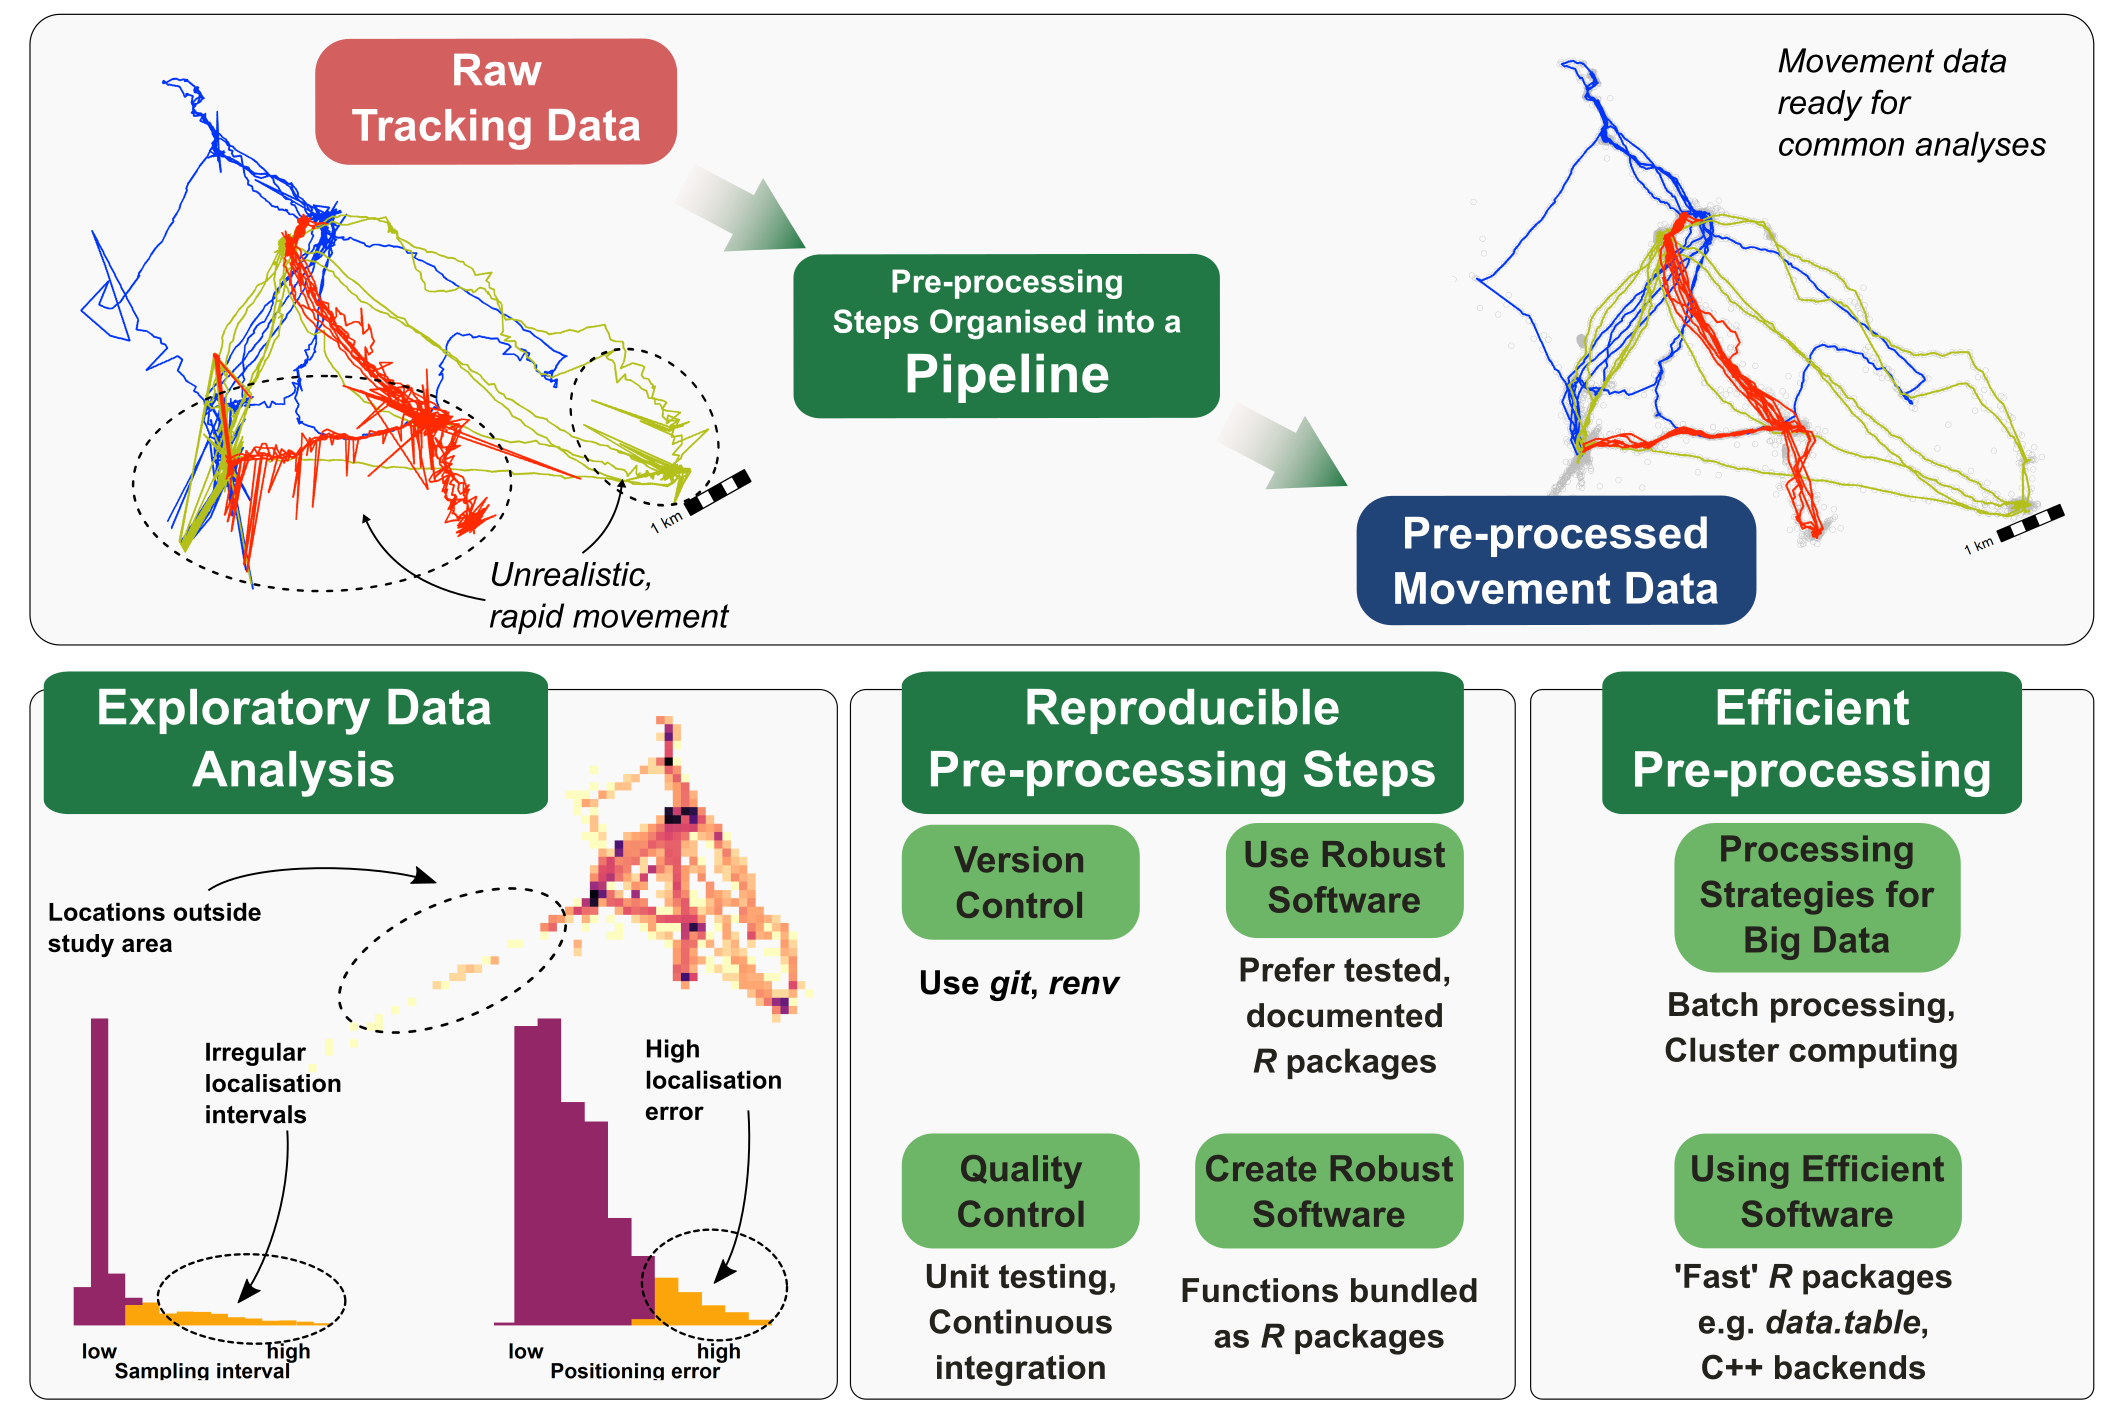
\includegraphics[width=0.7\textwidth]{figures/preprocessing/fig_01.png}
        \caption{
            \textbf{Some best-practices for pre-processing high-throughput tracking data.}
            Simple pre-processing of animal tracking data can improve the quality of animal tracking data, and the inferences that are drawn from it.
            % The organisation of pre-processing workflows into a `pipeline' --- a set of steps that users apply to prepare the data for a specific analysis --- can help make research more reproducible and reliable.
            Exploratory data analysis of representative subsets of the data can help to identify common issues with data quality, and to determine which pre-processing, steps such as filters and smooths, might be necessary (\textit{see also Fig.~\ref{preproc_fig_02}}).
            Pre-processing steps implemented as programming code can be made reproducible and shareable by following best-practices for software development: (i) tracking changes to the steps, and the software used, using version control (e.g. \textit{git}, \textit{renv}), (ii) preferring pre-existing tools, such as \textit{R} packages, which are well documented and tested, (iii) encapsulating custom-written code as functions, and bundling related functions into a package, and (iv) checking the quality of both custom-written code (e.g. by testing functions), and the overall pipeline (e.g. data visualisation).
            The efficiency of pre-processing steps can be increased by using strategies for dealing with large datasets, such as batch processing, or using a computing cluster.
            The use of existing tools optimised for large datasets, or by writing code in a `fast' language such as \textit{C++}, can also speed up the pre-processing of large datasets (see main text for examples).
            % See the \textit{Worked Out Example} on Egyptian fruit bats, as well as Supplementary Material 1, for more details on implementing pipelines.
            % Fig.~\ref{preproc_fig_02} shows an example of such a pipeline.
        }
        \label{preproc_fig_01}
    \end{sidewaysfigure}
% }

\afterpage{
    \begin{sidewaysfigure}[p]
        \centering
        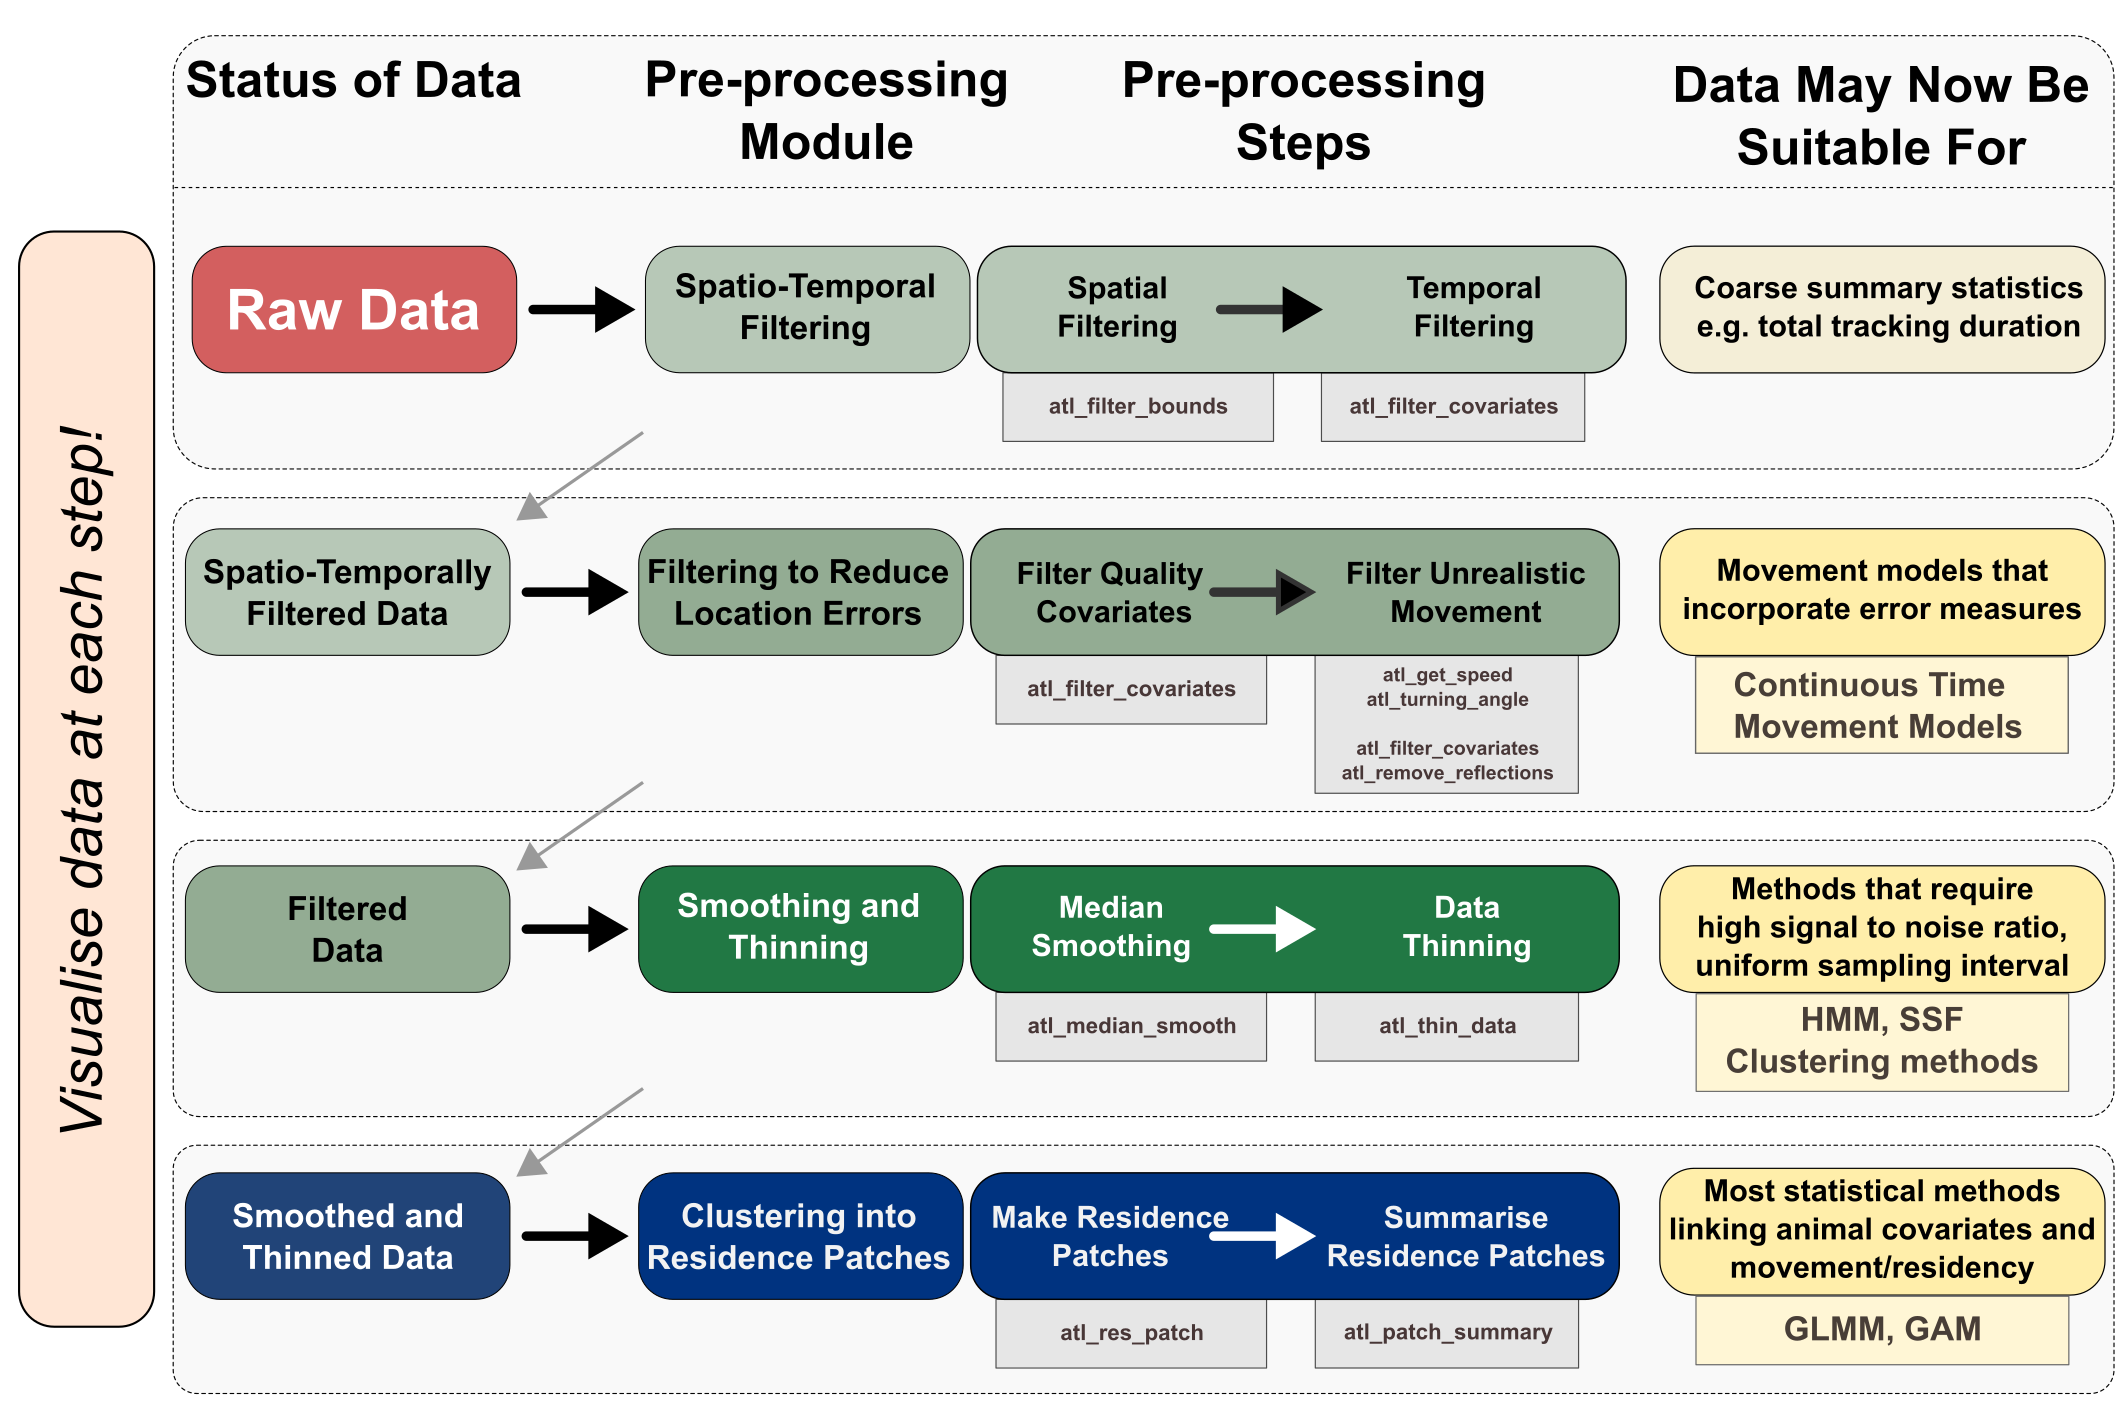
\includegraphics[width=0.7\textwidth]{figures/preprocessing/fig_02.png}
        \caption{
            \textbf{An example of a modular pipeline for pre-processing high-throughput tracking data from raw localisations to cleaned data, and optionally into residence patches.}
            Users should apply the appropriate pre-processing modules and the steps therein until the data are suitable for their intended analysis, some of which are suggested here.
            The \textit{atlastools} function that may be used to implement each pre-processing step is shown in the grey boxes underneath each step.
            Popular statistical methods are shown underneath possible analyses (yellow boxes).
            Users are strongly encouraged to visualise their data and scan it for location errors as they work through the pipeline, always asking the question, could the animal plausibly move this way?
        }
        \label{preproc_fig_02}
    \end{sidewaysfigure}
}

\section*{Best-Practices for Pre-Processing Workflows}

Exploratory data analysis should be the first step towards pre-processing movement data \citep[see Fig.~\ref{preproc_fig_01};][]{slingsby2016}.
Researchers with very large datasets of perhaps millions of rows should ideally select a representative subset of these data for exploratory data analysis, including individuals of different species, sexes, or seasonal cohorts.
Examples of exploratory data analysis include plotting heatmaps of the number of observations per unit area across the study site (Fig.~\ref{preproc_fig_01}).
Histograms of the location error estimates, plotting the linear approximations of animal paths between observations, and histograms of the sampling interval can help determine how data need to be treated so as to minimise location errors and improve computational tractability (Fig.~\ref{preproc_fig_01}).
While pre-processing steps required for datasets will differ between studies and tracking technologies, we elaborate upon candidate steps and their parameterisation in following sections (see also Fig.~\ref{preproc_fig_02}).

Following exploratory data analysis and the parameterisation of data cleaning steps, the specific implementation of these steps should be made reliable and reproducible.
Since reproducing pre-processing steps can be challenging when using only written descriptions from published articles, providing the code to implement pre-processing steps reduces ambiguity and increases reproducibility \citep{haddaway2015}.
For technically advanced users, the best-practices here are \textit{(i)} to implement pre-processing steps as `functions', \textit{(ii)} to collect related functions --- e.g. for similar kinds of data --- into a software `package', \textit{(iii)} to `test' that the functions handle input as expected, and \textit{(iv)} implement `version control' throughout, such that the process of development is documented \citep[Fig.~\ref{preproc_fig_01};][]{wickham2015,alston2020,perez-riverol2016}.

As an example, our \textit{atlastools} package incorporates these best-practices, and may be used as a reference \citep[][]{gupte2020a}.
We have written each pre-processing step as a separate function, and each of these functions is tested, usually on simulated data, but in some cases also on empirical data \citep[][see the directory \textit{tests/} in the associated Zenodo repository]{wickham2015}.
Finally, logging error messages is crucial when passing data through a pipeline, helping determine which data subsets could not be handled as expected, and why.
Users who would prefer to rely on pre-existing toolsets and methods can use \textit{R} packages that follow these best-practices, such as \textit{move} \citep{kranstauber2011}, and \textit{sftrack} \citep{boone2020}.
The large size of modern, high-throughput animal tracking data means that the computational challenge can often be \textit{the} main challenge in working with these data.
For beginning users, organising their workflows so that they process subsets of the data (such as one individual) at a time can help overcome limitations on working memory.
Animal tracking data stored in a relational database \citep[e.g. SQL databases][]{codd1970}, for example, can be broken into meaningful subsets based on individual identity and tracking season.
These smaller subsets can then be loaded into working memory, pre-processed, and saved in a separate location (see Supplementary Material 1, Section 2 for a worked out example on an SQL database).
Using existing tools optimised for tabular data, such as the \textit{R} package \textit{data.table} \citep{dowle2020}, can also speed up computation; \textit{atlastools} is built using \textit{data.table} for this reason.

More advanced users seeking substantial speed gains might wish to look into parallel-processing, and process each subset of the data independently of the full dataset, for example by using a computing cluster \citep[see also][for an alternative]{zjdai2021}.
Finally, another advanced method, used by popular packages such as \textit{move} \citep{kranstauber2011} and \textit{recurse} \citep{bracis2018}, is to write one's own methods in a `fast' low-level language, such as \textit{C++}, and link these to \textit{R} \citep[][]{eddelbuettel2013}; see also \textit{adehabitatLT}, which is written partially in \textit{C} \citep{calenge2006}.
Beginning practitioners can organise their workflows around these packages to benefit from the features they incorporate.

\section*{Pre-processing Steps, Usage, and Simulating Data}

\subsection*{An Overview of Pre-processing Steps and `atlastools'}

In the sections that follow, we lay out pre-processing techniques for raw high-throughput tracking data, and demonstrate working examples of these techniques, which we have collected in the \textit{R} package \textit{atlastools} (see Fig.~\ref{preproc_fig_02}).
Our package is aimed at getting `raw data' to the `analysis' stage identified by Joo et al. (2020) in their review of \textit{R} packages in movement ecology.
The package is based on \textit{data.table}, a fast implementation of data frames; thus it is compatible with a number of data structures from popular packages including \textit{move}, \textit{sftrack}, and \textit{ltraj} objects, which can be converted to data frames \citep[][]{kranstauber2011,boone2020,calenge2009}.
Our package functions are suitable for use with both regularly sampled data, as well as data with missing observations.

We cover, first, the use of simple \textit{\textbf{Spatio-Temporal Filters}} to select positions within a certain time or area.
Next, we show how users can \textit{\textbf{Reduce Location Errors}} by removing unreliable positions based on a system-specific error measure, or by the plausibility of associated movement metrics, such as speed and turning-angle \citep{seidel2018, calenge2009}.
We then show how users can tackle small-scale location errors by applying a \textit{\textbf{Median Smooth}}, and users who need uniformly sampled data, can undertake \textit{\textbf{Data Thinning}} by either aggregation or subsampling.
At this stage, the data are ready for a number of popular statistical treatments such as Hidden Markov Model-based classification \citep{michelot2016,langrock2012}.
Finally, we show how users wishing simple, efficient segmentation-clustering of points where the animal showed prolonged residence, can classify their data into `residence patches' \citep{barraquand2008, bijleveld2016} based on the movement ecology of their study species, after filtering out travelling segments (see \textit{\textbf{System-Specific Pre-Processing Tools}}).

These pre-processing techniques and package were designed with ATLAS systems in mind, motivated to meet the rapid growth of studies using this high-throughput system worldwide: in Israel \citep{toledo2014, toledo2016, toledo2020, corl2020, vilk2021}, the UK \citep{beardsworth2021a, beardsworth2021b}, and the Netherlands \citep[][]{beardsworth2022mee,bijleveld2021}. 
However, the principles and functions presented here are ready for use with other massive high-resolution data collected by GPS \citep[e.g.][]{papageorgiou2019}, reverse-GPS \citep[e.g.][]{aspillaga2021} or any other high-throughput tracking system .
Users may construct a pre-processing pipeline comprising of all the techniques we cover, or implement the modules most suitable for their data.
Users are advised to visualise their data throughout their workflow, and especially to perform thorough exploratory data analysis, to check for evident location errors or other issues \citep{slingsby2016}.


\subsection*{Simulating Data to Demonstrate Pre-Processing Steps}

To demonstrate pre-processing steps, we simulated a realistic movement track of 5,000 positions using an unbiased correlated velocity model (UCVM) implemented via the \textit{R} package \textit{smoove} \citep[][see Fig.~\ref{preproc_fig_03}.a]{gurarie2017}.
We added four kinds of error to the simulated track: (i) normally distributed small-scale offsets to the X and Y coordinates (small-scale error), (ii) normally distributed large-scale offsets to a random subset (0.5 \%) of the positions (spikes), (iii) large-scale displacement of a continuous sequence of 300 of the 5,000 positions (prolonged spikes; indices 500 -- 800), and (iv) we removed 10\% of the canonical track to simulate missing data (see Fig.~\ref{preproc_fig_03}.a).
To demonstrate the residence patch method, we obtained data, in the form of 1,000 positions, from a mechanistic, individual-based simulation model, in which agents move using simple decision making rules, and can find high-productivity patches using only ephemeral cues, such as the density of prey-items and other competitors \citep{gupte2021a, netz2022a}.
The emergent, complex track structure is analogous to the foraging movements of animals, and provides a suitable challenge for the residence patch method and helps to demonstrate its generality.

\section*{Spatio-Temporal Filtering}

\subsection*{Spatial Filtering Using Bounding Boxes and Polygons}

First, users should exclude positions outside the spatial bounds of a study area by comparing position coordinates with the range of acceptable coordinates (the bounding box), and removing positions outside them (Fig.~\ref{preproc_fig_03}.a). 
A bounding box filter does not require a geospatial representation such as a shapefile, and can help remove unreliable data from a tracking system that is less accurate beyond a certain range \citep[][]{beardsworth2022mee}.
In some special cases, users may wish to remove positions \textit{inside} a bounding box, either because movement behaviour within an area is not the focus of a study, or because positions recorded within an area are known to be erroneous.
An example of the former is studies of transit behaviour between features which can be approximated by their bounding boxes. 
Instances of the latter are likely to be system specific, but are known from ATLAS systems. 
Bounding boxes are typically rectangular, and users seeking to filter for other geometries, such as a circular or irregularly-shaped study area, need a geometric intersection between their data and a spatial representation of the area of interest (e.g. shapefile, geopackage, or \textit{sf}-object in \textit{R}).
The \textit{atlastools} function \textit{atl\_filter\_bounds} implements both bounding box and explicit spatial filters, and accepts X and Y coordinate ranges, an \textit{sf}-polygon or multi-polygon object \citep{pebesma2018}, or any combination of the three to filter the data.
When both coordinate ranges and a polygon are provided, the data is first filtered by the ranges and then the polygon.
The boolean function argument \textit{remove\_inside} determines whether positions inside the bounds are retained (\textit{FALSE}) or removed (\textit{TRUE}).

% \begin{lst{\color{red} Listing}}[float,floatplacement=h!,language=R, style=customR, caption = {
%     The \textit{atl\_filter\_bounds} function filters on an area defined by coordinate ranges, a polygon, or all three; it can remove positions outside (\textit{remove\_inside = FALSE}), or within the area (\textit{remove\_inside = TRUE}).
%     The arguments \textit{x} and \textit{y} determine the X and Y coordinate columns, \textit{x\_range} and \textit{y\_range} are the filter bounds in a coordinate reference system in metres, and the data can be filtered by an \textit{sf-(MULTI)POLYGON}, which can be passed using the \textit{sf\_polygon} argument. 
%     The output is a \textit{data.table}, which must be saved as an object (here, \textit{filtered\_data}).}]
% filtered_data <- atl_filter_bounds(
%                         data = data,
%                         x = "X", y = "Y",
%                         x_range = c(x_min, x_max),
%                         y_range = c(y_min, y_max),
%                         sf_polygon = your_polygon,
%                         remove_inside = FALSE
%                     )
% \end{lst{\color{red} Listing}}

\begin{figure}[ht!]
    \centering
    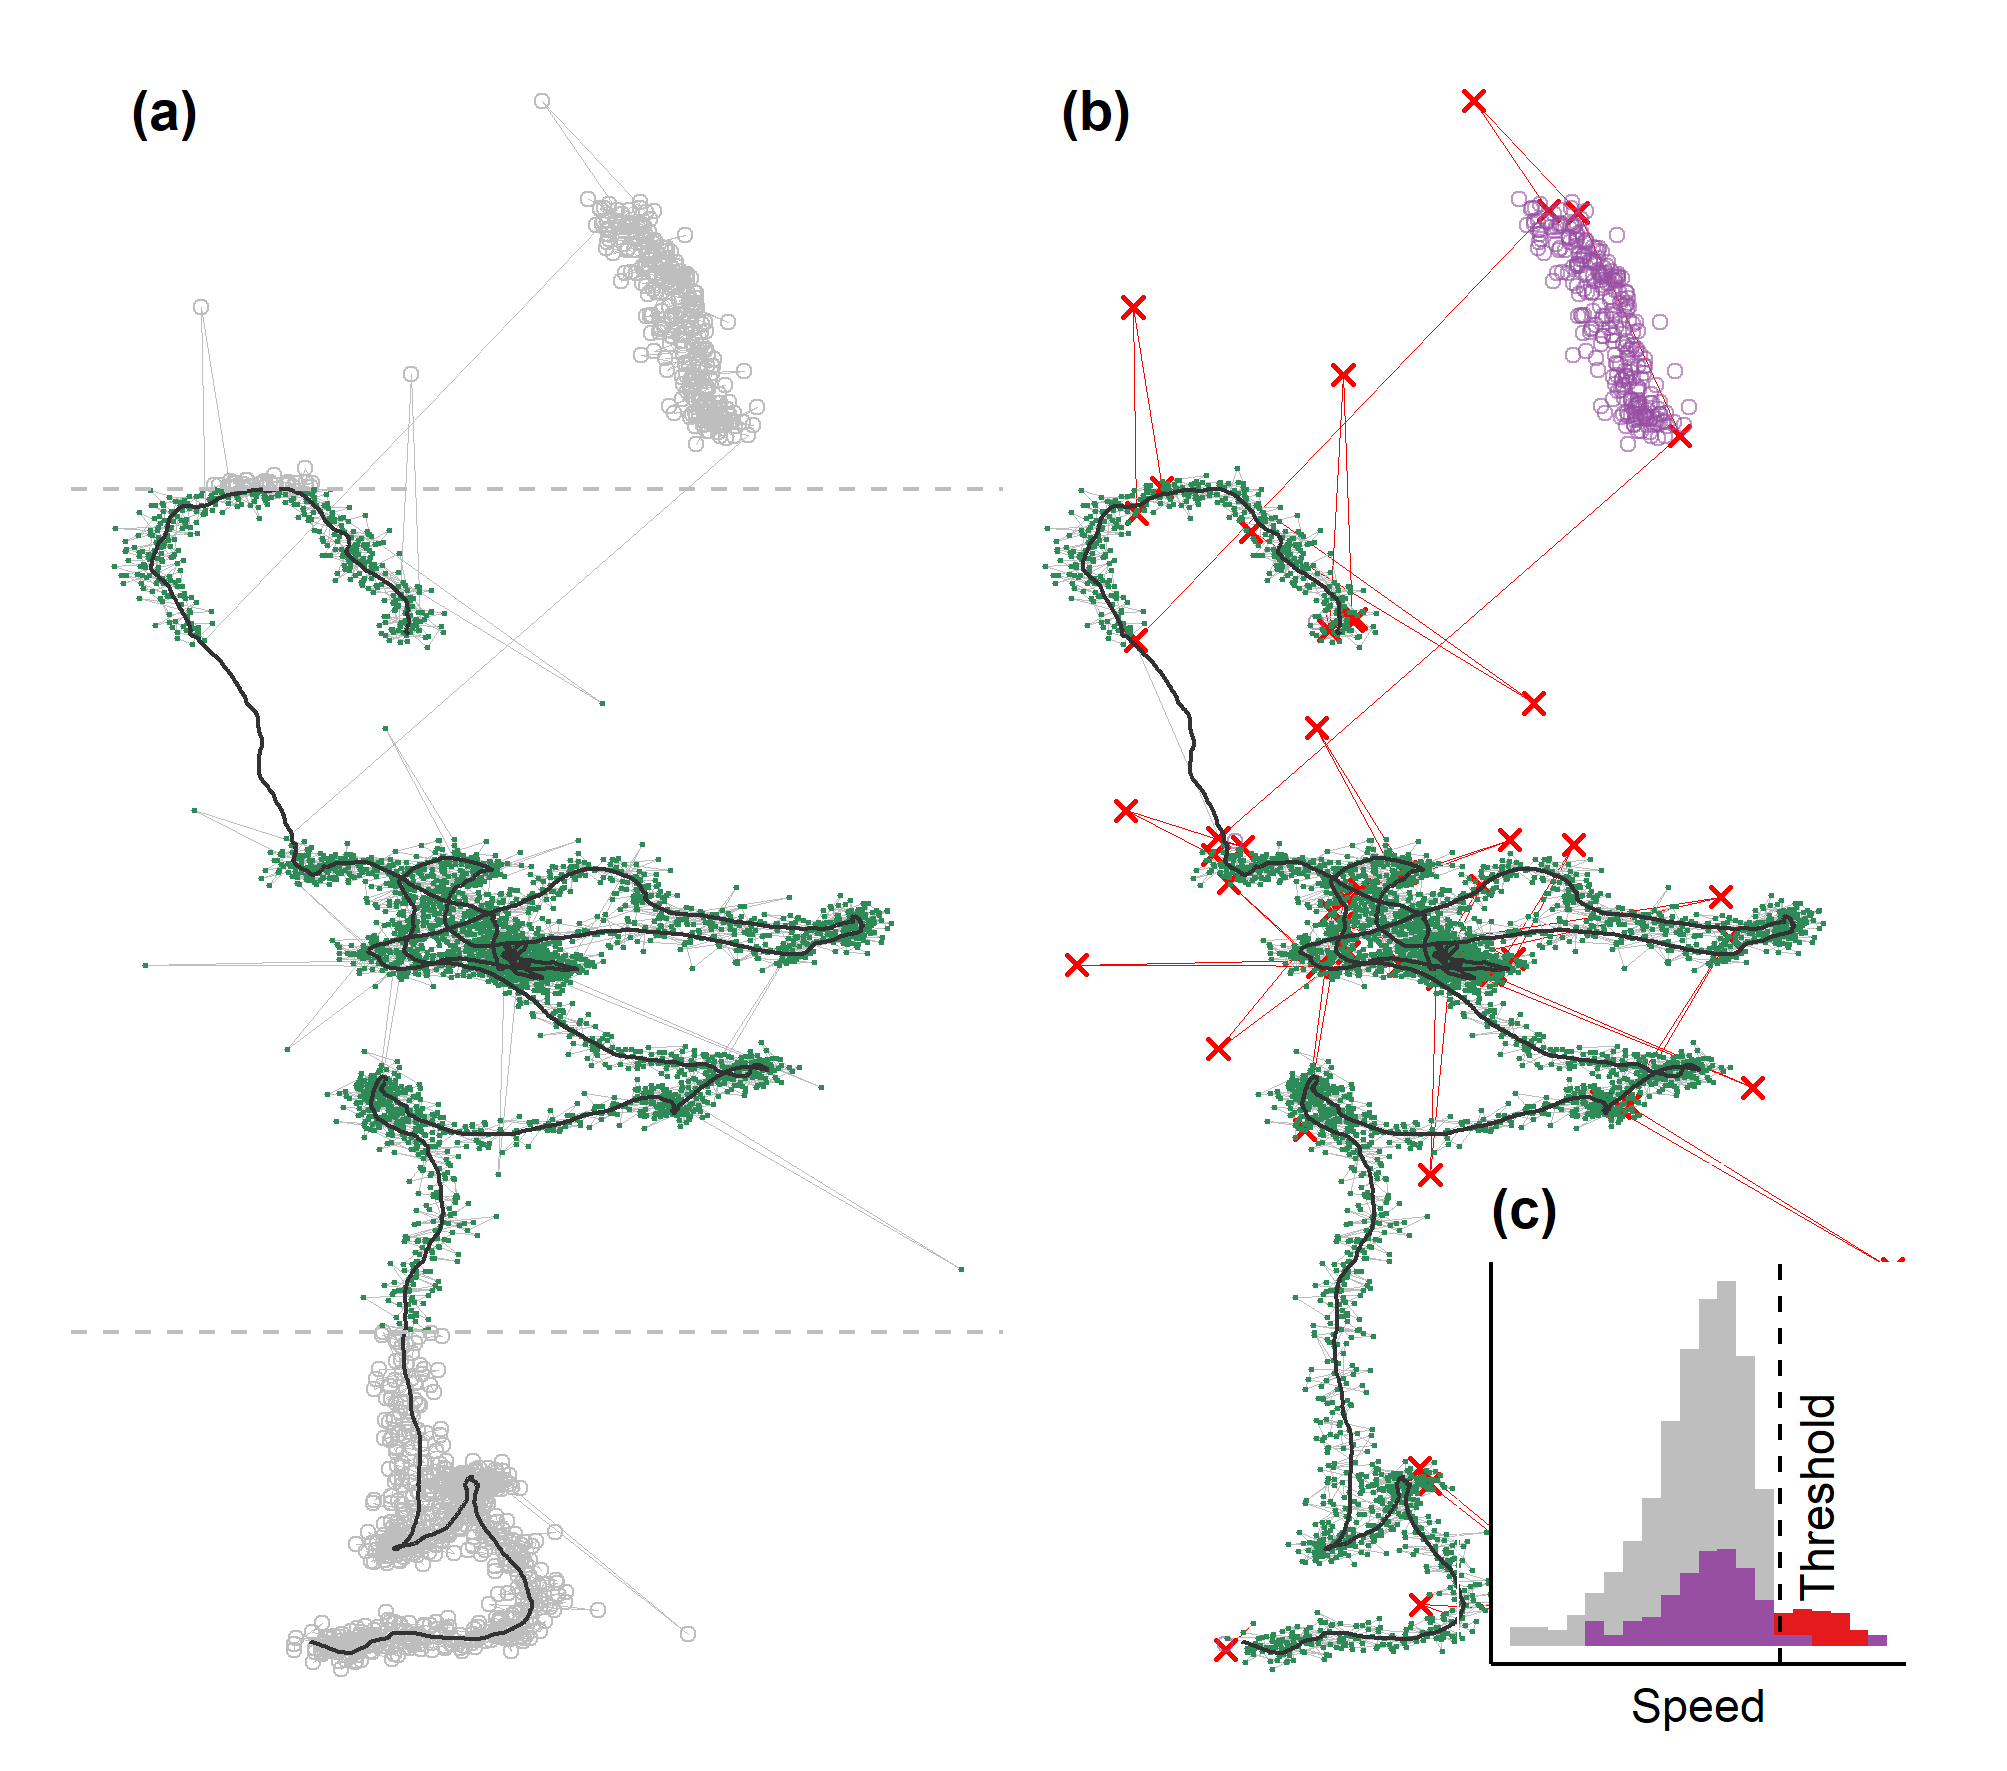
\includegraphics[width=0.9\textwidth]{figures/preprocessing/fig_03.png}
    \caption{
        \textbf{Simulated movement data showing four kinds of artificially added errors}.
        (i) Normally distributed small-scale error on each position, (ii) large-scale error added to 0.5\% of positions, (iii) 10\% of positions removed to simulate missing data, and (iv) 300 consecutive positions displaced to simulate a gross distortion affecting a continuous subset of the track.
        \textbf{(a)} Tracks can be quickly filtered by spatial bounds (dashed grey lines) to exclude broad regions (green = retained; grey = removed).
        \textbf{(b)} location error may affect single observations resulting in point outliers or `spikes' (red crosses and track segments), or continuous subsets of a track, called a `prolonged spike' (purple circles, top right), and both represent unrealistic movement.
        \textbf{(c)} Histograms of speed for the track (grey = small-scale errors, red = spikes), and the prolonged spike (purple) show that while spikes could be removed by filtering out positions with both high incoming and outgoing speeds and turning angles, prolonged spikes cannot be removed in this way, and should be resolved by conceptualising algorithms that find the bounds of the distortion instead.
        Users should frequently check the outputs of such algorithms to avoid rejecting valid data.
    }
    \label{preproc_fig_03}
\end{figure}

\subsection*{Temporal and Spatio-temporal Filters}

Tracking data might fail to properly represent an animal's movement at certain times, for instance, data recorded before release, or data from shortly after release when the animal is still influenced by the stress of capture and handling.
Periods of poor tracking quality may result from system malfunctions and unusual disturbances, and users may wish to exclude these data as well.
Temporal filtering can exclude positions from intervals when data are expected to be unreliable for ecological inference, either due to abnormal movement behaviour or system-specific issues.  
Temporal filters can be combined with spatial filters to select specific time-location combinations. 
For example, studies of foraging behaviour of a nocturnal animal would typically exclude tracking data from the animal's daytime roosts (see \textit{Worked Out Example}).
Users should apply filters in sequence rather than all at once, and visualise the output after each filtering step (`sanity checks'; see Supplementary Material Section 2).
The atlastools function \textit{atl\_filter\_covariates} allows convenient filtering of a dataset by any number of logical statements, including querying data within a spatio-temporal range.
% This function can be used to easily filter timestamps in a range, as well as combine simple spatial and temporal filters.
% It accepts a character vector of \textit{R} expressions that each return a logical vector (i.e., \textit{TRUE} or \textit{FALSE}; {\color{red} Listing} 2).
The function keeps only those data which satisfy each of the filter conditions, and users must ensure that the filtering variables exist in their dataset in order to avoid errors.

% \begin{lst{\color{red} Listing}}[float, language=R, style=customR, caption = {
%     Data can be filtered by a temporal or a spatio-temporal range using \textit{atl\_filter\_covariates}. 
%     Filter conditions are passed to the \textit{filters} argument as a character vector. 
%     Only rows in the data satisfying \textit{all} the conditions are retained. 
%     Here, the first example shows how nighttime data can be retained using a predicate that determines whether the value of `hour' is between 6 and 18, and also within a range of X coordinates.
%     The second example retains ATLAS locations calculated using $>$ 3 base stations (\textit{NBS}), with location error (\textit{SD}) $<$ 100, and data between an arbitrary day 5 and day 8.
%     }]
% night_data <- atl_filter_covariates(
%                     data = dataset,
%                     filters = c(
%                         "!inrange(hour, 6, 18)",
%                         "between(x, x_min, x_max)"
%                     )
%                 )

% filtered_data <- atl_filter_covariates(
%                         data = data,
%                         filters = c(
%                             "NBS > 3",
%                             "SD < 100",
%                             "between(day, 5, 8)"
%                         )
%                     )                            
% \end{lst{\color{red} Listing}}

\section*{Filtering to Reduce Location Errors}

\subsection*{Filtering on Data Quality Attributes}

Tracking data attributes can be good indicators of the reliability of positions calculated by a tracking system \citep{beardsworth2022mee}.
GPS systems provide direct measures of location error during localisation \citep[Horizontal Dilution of Precision, HDOP in GPS]{ranacher2016}, while  in reverse-GPS systems, a measure referred to as Standard Deviation (SD in many datasets), can be calculated from the variance-covariance matrix of each position as: $\text{SD} = \sqrt{\text{Var X} + \text{Var Y} + \text{Cov XY}}$ \citep[see details in][]{maccurdy2009, maccurdy2019, weiser2016, ranacher2016}.
Tracking data can also include indirect indicators of data quality.
For instance, GPS systems' location error may be indicated indirectly by the number of satellites involved in the localisation.
In reverse-GPS systems too, the number of base stations involved in each localisation is an indirect indicator of data quality, and positions localised using more receivers are usually more reliable \citep[the minimum required for an ATLAS localisation is 3; see][]{weiser2016,beardsworth2022mee}.
A location error measure associated with each coordinate pair (similar to GPS HDOP) can be calculated and assigned to a new column \textit{SD} using the formula for the sum of correlated random variables
\begin{linenomath*}
    \begin{equation*}
        SD = \sqrt{{VARX} + {VARY} + 2 \times {COVXY}}
     \end{equation*}
\end{linenomath*}
Unreliable positions can be removed by filtering on direct or indirect measures of quality using \textit{atl\_filter\_covariates}.
While filtering on direct quality attributes and unrealistic movement speeds (see below) will often be sufficient, filtering on indirect quality indicators is a strategy to consider when direct error measures are not available.

\subsection*{Filtering Unrealistic Movement}

Filtering on system-generated attributes may not remove all erroneous positions, and the remaining data may still include biologically implausible movement.
Users are encouraged to visualise their tracks before and after filtering point locations, and especially to `join the dots' and connect consecutive positions with lines (Fig.~\ref{preproc_fig_03}.b).
Whether the resulting track looks realistic is ultimately a subjective human judgement, but any decision to filter-out data must remain independent of the hypothesised movement behavior.
This basic principle does not preclude explicitly integrating prior knowledge of the movement ecology of the study species to ask, `Does the animal move this way?'.
Segments which appear to represent unrealistic animal movement are often obvious to researchers with extensive experience of the study system \citep[the non-movement approach; see][]{bjorneraas2010}.
Since it is both difficult and prohibitively time consuming to exactly reproduce expert judgement when dealing with large volumes of tracking data from multiple individuals, some automation is necessary.
Users should first manually examine a representative subset of tracks and attempt to visually identify problems --- either with individual positions, or with subsets of the track --- that persist after filtering on system-generated attributes.
Once such problems are identified, users can conceptualise algorithms that can be applied to their data to resolve them.

A common example of a problem with individual positions is that of point outliers or `spikes' \citep{bjorneraas2010}, where a single position is displaced far from the track (see Fig.~\ref{preproc_fig_03}.b).
Point outliers are characterised by artificially high speeds between the outlier and the positions before and after \citep[called incoming and outgoing speed, respectively;][]{bjorneraas2010}, lending a `spiky' appearance to the track.
Removing spikes is simple: remove positions with extreme incoming and outgoing speeds.
Users must first define plausible upper limits of the study species' speed \citep{calenge2009, seidel2018}.
Here, it is important to remember that speed estimates are scale-dependent; high-throughput tracking typically overestimates the speed between positions where the animal is stationary or moving slowly, due to small-scale location errors \citep{ranacher2016, noonan2019}. 
Even after data with large location errors have been removed, it is advisable to begin with a liberal (high) speed threshold that excludes only the most unlikely speeds.
Estimates of maximum speed may not always be readily obtained for all species, and an alternative is to use a data-driven threshold such as the 90\textsuperscript{th} percentile of speeds from the track.
Once a speed threshold $S$ has been chosen, positions with incoming \textit{and} outgoing speeds $> S$ may be identified as spikes and removed.

Some species can realistically achieve speeds $> S$ in fast transit segments when assisted by their environment, such as birds with tailwinds, and a simple filter on incoming and outgoing speeds would exclude this valid data.
To avoid removing valid, fast transit segments while still excluding spikes, the speed filter can be combined with a filter on the turning angles of each position \citep[see][]{bjorneraas2010, calenge2009}.
This combined filter assumes that positions in high-throughput tracking with both high speeds and large turning angles are likely to be due to location errors, since most species are unable to turn sharply at very high speed.
Users can then remove those positions whose incoming and outgoing speeds are both $> S$, and where $\theta > A$ (sharp, high-speed turns), where $\theta$ is the turning angle, and $A$ is the turning angle threshold.
Many other track metrics may be used to identify implausible movement and to filter data \citep{seidel2018}.
At this early stage in pre-processing, track metrics should be considered provisional --- it is not until after smoothing and potentially resampling to a regular interval (see below), that calculated track metrics should be used for ecological inference.
% We show an implementation of spike removal using the \textit{atl\_filter\_covariates} function.

% \begin{lst{\color{red} Listing}}[float, language=R, style=customR, caption = {
%     Filtering a movement track on incoming and outgoing speeds, and on turning angle to remove unrealistic movement.
%     The functions \textit{atl\_get\_speed} and \textit{atl\_turning\_angle} are used to get the speeds and turning angles before filtering, and assigned to a column in the data (assignment of \textit{speed\_out} is not shown).
%     The filter step only retains positions with speeds below the speed threshold $S$ \textit{or} angles above the turning angle threshold $\theta$, i.e., positions where the animal is slow but makes sharp turns, and data where the animal moves quickly in a relatively straight line.}]
% data$speed_in <- atl_get_speed(
%                     data,
%                     x = "x", y = "y",
%                     time = "time", 
%                     type = c("in")
%                 )

% data$angle <- atl_turning_angle(
%                     data,
%                     x = "x", y = "y", 
%                     time = "time"
%                 )

% filtered_data <- atl_filter_covariates(
%                     data = data,
%                     filters = c(
%                         "(speed_in < S & speed_out < S) | angle < A"
%                     )
%                 )
% \end{lst{\color{red} Listing}}

Sometimes, entire subsets of the track may be affected by the same large-scale location error.
For instance, multiple consecutive positions may be roughly translated (geometrically) away from the real track and form `prolonged spikes', or `reflections' (see Fig.~\ref{preproc_fig_03}.b).
These cannot be corrected by targeted removal of individual positions, as in Bjørneraas et al.'s approach (2010), since there are no positions with both high incoming and outgoing speeds, as well as sharp turning angles, that characterise spikes.
Since filtering individual positions will not suffice, algorithms to correct such errors must take a track-level view, and target the displaced sequence overall.
Track-subset algorithms are likely to be system-specific, and may be challenging to conceptualise or implement.
In the case of prolonged spikes, one relatively simple solution is identifying the bounds of displaced segments, and removing positions between them.
This identification can be based on relatively simple rules --- for example, the beginning of a prolonged spike could be identified as a position with a high \textit{incoming} speed, but a low \textit{outgoing} speed, while the end of such a spike would have a low incoming, but a high outgoing speed.
We have implemented an illustrative example of such an algorithm in the form of track-subset filtering for prolonged spikes using the \textit{atlastools} function \textit{atl\_remove\_reflections} (see the \textit{atlastools} documentation for details on the algorithm).
Users are strongly encouraged to visualise their data before and after applying such algorithms; as these methods are not foolproof, and data that are heavily distorted by errors affecting entire track-subsets should be used with care when making further inferences.

% % \begin{lst{\color{red} Listing}}[float, language=R, style=customR, caption = {
% %     Removing unrealistic movement in the form of prolonged spikes from a movement track. 
% %     The important function arguments here are \textit{point\_angle\_cutoff} ($A$), \textit{reflection\_speed\_cutoff} ($S$), and \textit{est\_ref\_len}, the maximum number of positions after the inner bound that are candidates for the end of the prolonged spike, i.e., the outer bound. 
% %     If the prolonged spike ends after less than $N$ positions, the true end point is used as the outer bound of the spike.
% %     However, the algorithm behind this function fails when the prolonged spike ends after more than $N$ positions. 
% %     Users are advised to use a liberally large value of N in the \textit{est\_ref\_len} argument; 1,000 may be appropriate for 3s interval data.
% %     Further, users are cautioned against relying on such algorithms for severely distorted data.}]
% % filtered_data <- atl_remove_reflections(data = track_data,
% %                        x = "x", y = "y", time = "time",
% %                        point_angle_cutoff = A,
% %                        reflection_speed_cutoff = S,
% %                        est_ref_len = N)
% % \end{lst{\color{red} Listing}}

\section*{Smoothing and Thinning Data}

\subsection*{Median Smoothing}

After filtering out large location errors, the track may still look `spiky' at small scales, and this is due to smaller location errors that are especially noticeable when the individual is stationary or moving slowly \citep{noonan2019}.
These smaller errors are challenging to remove since their attributes (such as speed and turning angles) are within the expected range of movement behaviour for the study species. 
The large data volumes of high-throughput tracking allow users to resolve this problem by smoothing the positions. 
The most basic `smooths' work by approximating the value of an observation based on neighbouring values.
For a one-dimensional series of observations, the neighbouring values are the $K$ observations centred on each index value $i$.
The range ${i - (K-1)/2} \ldots {i + (K-1)/2}$ is referred to as the moving window as it shifts with $i$, and $K$ is the moving window size.
A common smooth is nearest neighbour averaging, in which the value of an observation $x_i$ is the average of the moving window $K$.
The median smooth is a variant of nearest neighbour averaging which uses the median rather than the mean, and is more robust to outliers (\citeauthor{tukey1977} 1977).
The median smoothed value of the X coordinate, for instance, is
%
% \begin{linenomath*}
    % \begin{equation*}
    $$
        X_i = \text{Median}(X_{i - (K-1)/2} \ldots X_{i + (K-1)/2}).
    $$
        % \end{equation*}
% \end{linenomath*}
Users can apply a median smooth with an appropriate $K$ independently to the X and Y coordinates of a movement track to smooth it (see Fig.~\ref{preproc_fig_04}.a -- e).
The median smooth is robust to even very large temporal and spatial gaps, and does not interpolate between positions when data are missing. 
Thus it is not necessary to split the data into segments separated by periods of missing observations when applying the filter (see Fig.~\ref{preproc_fig_04}).

Some data sources, such as GPS, provide tracks that have already been smoothed in quite sophisticated ways, such as with a Kalman filter, making a median smooth unnecessary \citep{kaplan2005}.
Furthermore, smoothing is not a panacea for data quality issues, and has its drawbacks.
Smoothing does not change the number of observations, but does decouple the coordinates from some of their attributes.
For instance, smoothing breaks the relationship between a coordinate and the location error estimate around it (VARX, VARY, and SD in ATLAS systems).
Since the X and Y coordinates are smoothed independently, the smoothed coordinates of an observation will likely differ from all the coordinates used to compute the smoothed value.
Any position covariates (e.g. environmental values such as landcover or elevation) obtained before smoothing should be replaced with the covariates obtained at the smoothed coordinates.
Similarly, instantaneous track metrics, such as speed and turning angle, should also be updated at this stage to reflect the smoothed coordinates.
Furthermore, the location error estimate around each coordinate, and around the localisation overall, become invalid and should be ignored.
This makes subsequent filtering on measures of data quality unreliable, and smoothed data are unsuitable for use with methods that model location uncertainty \citep{noonan2019, fleming2014, fleming2020, calabrese2016}.
Thus, when applying location error modelling methods, users should ensure that the error measure bears a mechanistic relationship with the location estimate \citep[see][ for more details]{fleming2020, noonan2019}.
Additionally, excessively large $K$ may result in a loss in detail of the individual's small-scale movement (compare Fig.~\ref{preproc_fig_04}.e with ~\ref{preproc_fig_04}.a).
Users must themselves judge how best to balance large-scale and small-scale accuracy, and choose $K$ accordingly.
Median smoothing is provided by the \textit{atlastools} function \textit{atl\_median\_smooth}, with the only option being the moving window size, which must be an odd integer.

% \begin{lst{\color{red} Listing}}[float, language=R, style=customR, caption = {
%     Median smoothing a movement track using the function \textit{atl\_median\_smooth} function with a moving window \textit{K = 5}. 
%     Larger values of $K$ yield smoother tracks, but $K$ should always be some orders of magnitude lower than the number of observations.}]
% atl_median_smooth(
%     data = track_data,
%     x = "x", y = "y",
%     time = "time",
%     moving_window = 5
% )
% \end{lst{\color{red} Listing}}

\begin{figure}[ht!]
    \centering
    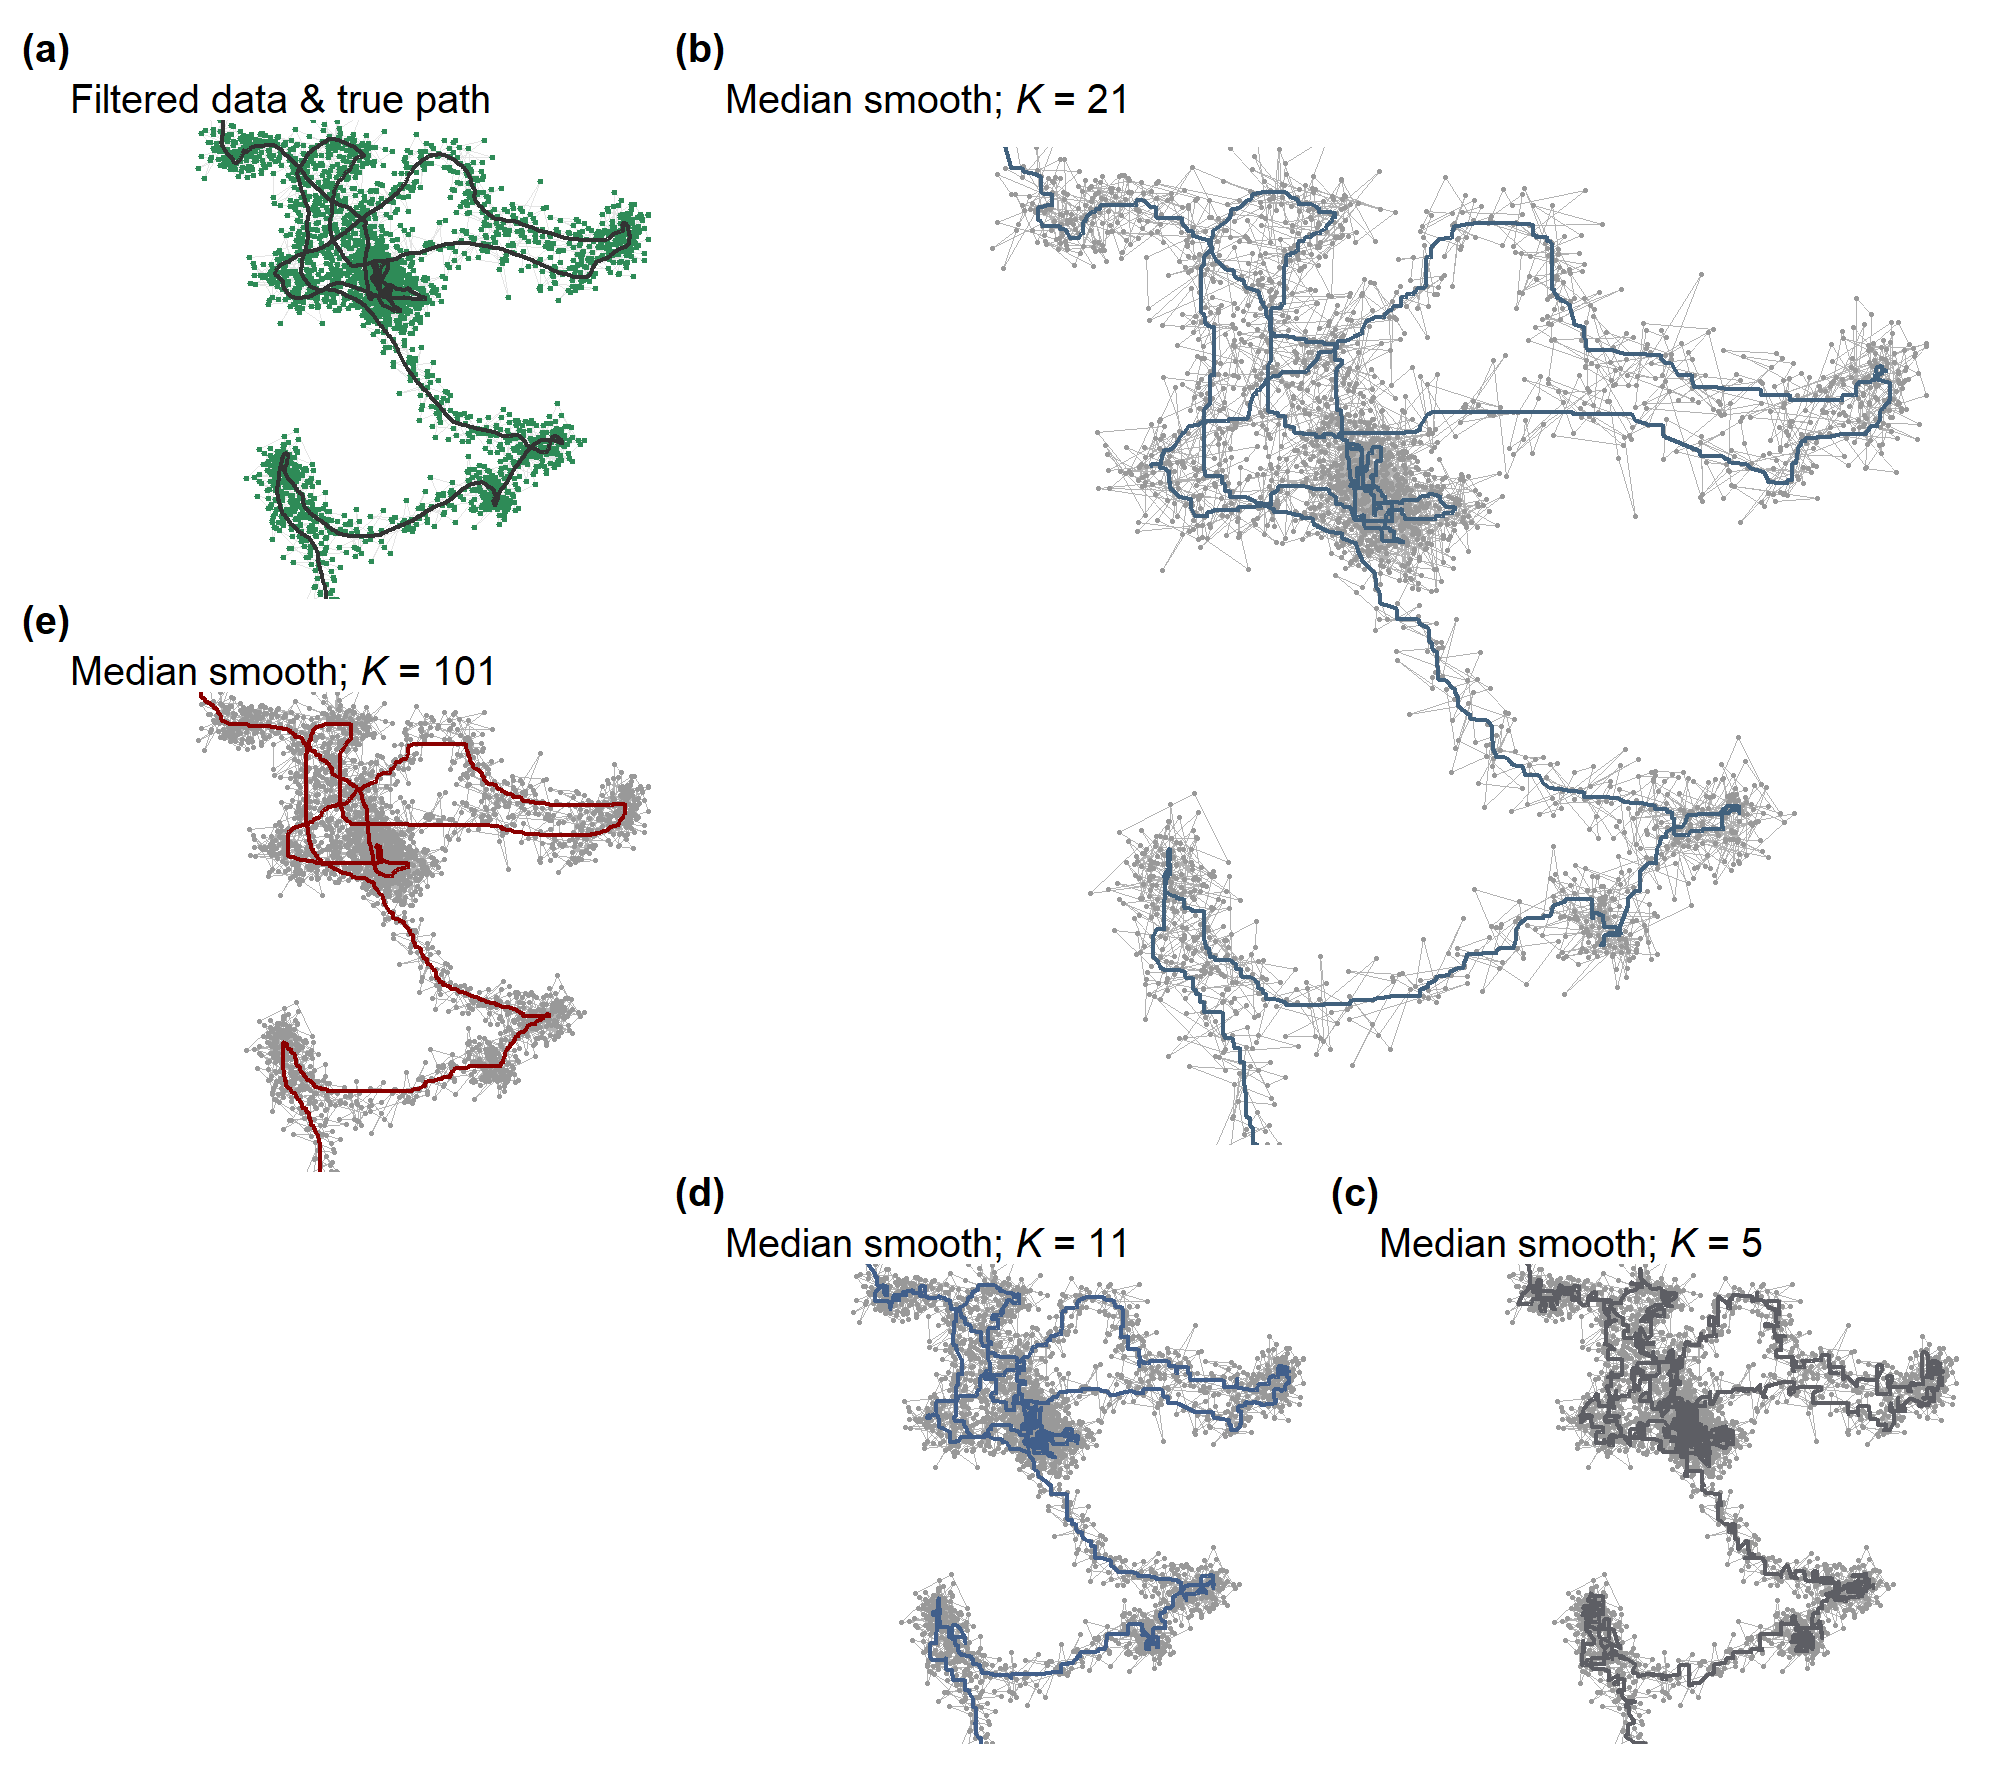
\includegraphics[width=0.9\textwidth]{figures/preprocessing/fig_04.png}
    \caption{
        \textbf{Median smoothing position coordinates reduces small-scale location error in tracking data.}
        The goal of this step is to approximate the simulated canonical track (black line, \textbf{(a)}), given positions with small-scale error that remains after filtering in previous steps (green points).
        \textbf{(b)} Median smoothing the position coordinates (green points, in \textbf{(a)}) over a moving window ($K$) of 21 positions gives a good approximation (blue line) of the canonical track, and is a significant improvement on the unsmoothed track (grey lines and points).
        While $K$ should usually be at least two orders of magnitude less than the number of positions in the track, users are cautioned that there is no correct $K$, and they must subjectively choose a $K$ which most usefully trades small-scale details of the track for large-scale accuracy.
        Here, smoothing with a $K$ of \textbf{(c)} 5 (dark grey line) and \textbf{(d)} 11 (blue line), leads to a jagged track, compared to the true path in (a), and the distance moved by the animal would be overestimated.
        \textbf{(e)} Using extremely large values of $K$ (101) may lead to a loss of both large and small scale detail (red line).
        Across panels, grey lines and points show the track without smoothing.
    }
    \label{preproc_fig_04}
\end{figure}

\subsection*{Thinning Movement Tracks}

Most data at this stage are technically ‘clean', yet the volume alone may pose challenges for lower-specification or older hardware and software if these are not optimised for efficient computation.
Thinning data i.e., reducing their volume, need not compromise researchers' ability to answer ecological questions; for instance, proximity-based social interactions lasting 1 -- 2 minutes would still be detected on thinning from a sampling interval of 1 second to 1 minute \citep[][]{aspillaga2021a}.
Thinning data also does not imply that efforts to collect high-throughput movement data are ‘wasted', as rich movement datasets enable more detailed and more accurate representation of the true track, as elaborated above. 
Indeed, some analyses require that temporal auto-correlation in the data be broken by subsampling the data to a lower resolution; these include traditional kernel density estimators for animal home-range, as well as resource selection functions \citep{fleming2014,manly2007,dupke2017}.
Furthermore, a number of powerful methods in movement ecology, including Hidden Markov Models and integrated Step-Selection Analysis recommend uniform sampling intervals \citep{avgar2016,langrock2012,michelot2016}.
Finally, subsampling data may be an important strategy in exploratory data analysis; for instance, it allows researchers to determine whether computationally intensive methods, such as distance and speed estimates from continuous time movement model fitting, are required for their data, or whether the movement metrics stabilise at a certain time scale \citep[][]{noonan2019}.
Two plausible approaches here are subsampling and aggregation, and both approaches begin with identifying time-interval groups (e.g. of 1 minute).
Subsampling picks one position from each time-interval group while aggregation involves computing the mean or median of all system-generated attributes for positions within a time-interval group.
Here again, users should repeat the extraction of any environmental covariates for the thinned data, and may wish to obtain the mean values in a radius aroung the locations, rather than point estimates alone.
Both approaches yield one position per time-interval group (Fig.~\ref{preproc_fig_05}.a).
Categorical variables, such as the habitat type associated with each position, can be aggregated using a suitable measure such as the mode.
We caution users that thinning causes an extensive loss of small-scale detail in the data, and should be used carefully.

Both aggregation and subsampling have their relative advantages. 
The aggregation method is less sensitive to selecting point outliers by chance than subsampling.
However, to account for location error with methods such as state-space models \citep{jonsen2003, jonsen2005, johnson2008} or continuous time movement models \citep{fleming2014, noonan2019, gurarie2017, calabrese2016, fleming2020}, correctly propagating the location error is important, and subsampling directly propagates these errors without further processing.
In reverse-GPS systems systems the location error is calculated from the variance-covariance matrix of the coordinates of candidate positions considered by the location solver \citep{weiser2016}; this is equivalent to GPS systems' HDOP \citep{ranacher2016}.
In the aggregation method, the location error around each coordinate provided by either GPS or reverse-GPS systems can be propagated --- assuming the errors are normally distributed --- to the averaged position as the sum of errors divided by the square of the number of observations contributing to each average ($N$):
% \begin{linenomath*}
    $$
        \text{Var}(X)_\text{agg} = \left( \sum_{i=1}^{i=N} \text{Var}(X)_i \right) / N ^ 2
    $$
% \end{linenomath*}
Similarly, the overall location error estimate for the average of $N$ positions in a time-interval can be calculated by treating it as a variance. For instance, the ATLAS error and GPS error measures (SD and HDOP, respectively) can be aggregated as:
% \begin{linenomath*}
    $$
        \text{SD}_\text{agg} \ or \ \text{HDOP}_\text{agg} = \sqrt{ \left( \sum_{i=1}^{i=N} \text{SD}_i^2 \ or \ \text{HDOP}_i^2 \right) / N ^ 2  }
    $$
% \end{linenomath*}

Users may question why thinning, which can obtain consensus positions over an interval and also reduce data-volumes should not be used directly on the raw data.
%%
We caution that thinning prior to excluding unrealistic movement and smoothing (Fig 5.b) can lead to preserving artefacts in the data, and estimates of essential metrics --- such as straight-line displacement (and hence, speed) --- that are substantially different from the true value \citep[see Fig.~\ref{preproc_fig_05}.c;][]{noonan2019}.
In our example, the data with errors would have to be thinned to $\frac{1}{30}$\textsuperscript{th} of its volume for the median speed of the thinned data to be comparable with the overall median speed --- this is an undesirable step if the aim is fine-scale tracking.
Additionally, the optimal level of thinning can be difficult to determine, especially if there is wide individual variation in movement behaviour, and the mis-estimation of track metrics from inappropriately thinned data could have consequences for the implementation of subsequent filters based on detecting unrealistic movement.
However, thinning before data-cleaning has its place as a useful step before exploratory visualisation of the movement track, since reduced data-volumes are easier to handle for plotting software.
%
Thinning is implemented in \textit{atlastools} using the \textit{atl\_thin\_data} function, with either aggregation or subsampling (specified by the \textit{method} argument) over an interval using the \textit{interval} argument.
Grouping variable names (such as animal identity) may be passed as a character vector to the \textit{id\_columns} argument.

% \begin{lst{\color{red} Listing}}[float, language=R, style=customR, caption = {Code to thin data by aggregation in \textit{atlastools}. The method can be either "aggregate" or "subsample". 
% The time interval is specified in seconds, while the \textit{id\_columns} allows a character vector of column names to be passed to the function, with these columns used as identity variables.
% Both methods return a dataset with one rows per time-interval.}]
% thinned_data <- atl_thin_data(
%                     data,
%                     interval = 60,
%                     id_columns = c("animal_id"),
%                     method = "aggregate"
%                 )
% \end{lst{\color{red} Listing}}

% % figure for aggregation thinning
\afterpage{
    \begin{sidewaysfigure}[p]
        \centering
        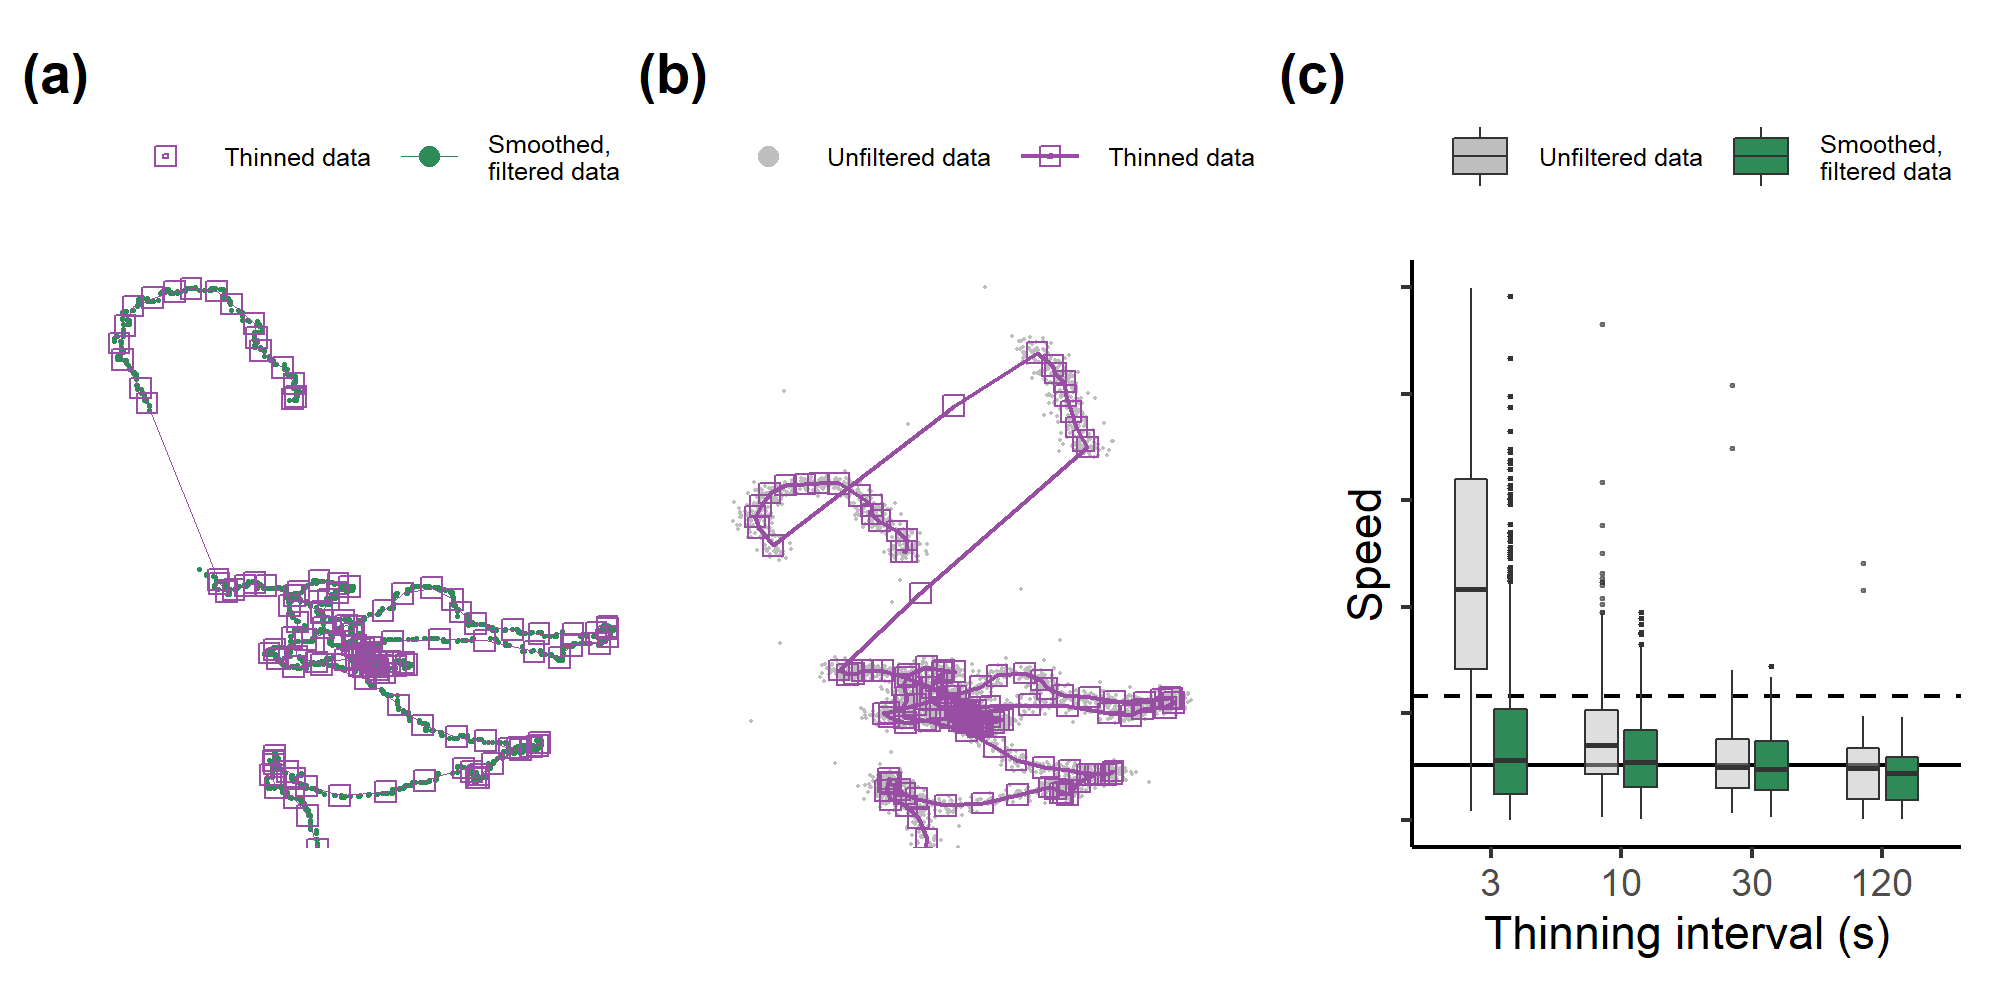
\includegraphics[width=0.7\textwidth]{figures/preprocessing/fig_05.png}
        \caption{
            \textbf{Thinning tracking data can aid computation but must be approached carefully}.
            Aggregating a filtered and smoothed movement track \textbf{(a)} preserves track structure while reducing data-volume, but \textbf{(b)} aggregating before filtering gross location errors and unrealistic movement leads to the persistence of large-scale errors (such as prolonged spikes).
            \textbf{(c)} Thinning before data cleaning can lead to significant misestimations of essential movement metrics such as speed at lower intervals.
            Boxplots show the median and interquartile ranges for speed estimates of tracks aggregated over intervals of 3, 10, 30, and 120 seconds.
            For comparison, the median and 95\textsuperscript{th} percentile of speed of the canonical track are shown as solid and dashed horizontal lines, respectively.
            % The unfiltered data would have to be thinned to \sfrac{1}{30}\textsuperscript{th} volume to correctly estimate median speed.
        }
        \label{preproc_fig_05}
    \end{sidewaysfigure}
}

\section*{System-Specific Pre-processing Tools}

When researchers' pre-processing requirements exceed the functionalities of existing tools, they might have to conceptualise and implement their own methods.
For instance, an important and common analysis with animal tracking data is to link space use with environmental covariates.
This is difficult even with smoothed and thinned high-throughput data, as these may be too large for statistical packages, or have strong autocorrelation.
Users aiming for such analyses can benefit from segmenting and clustering the data into spatio-temporally independent bouts of different behavioural modes \citep{patin2020a}.
Treating these as the unit of observation also conveniently sidesteps pseudo-replication and reduces computational requirements.
While numerous methods of segmenting and clustering data are in use, they may not be scalable to very large or gappy datasets \citep{patin2020a, langrock2012, michelot2016}.
As an alternative, a first-principles approach that segments data based on the movement capacity (top speed, etc.) of tracked animals, could provide a fast, yet useful way to cluster data.
Here, as a working example that may be suitable for some systems, we present a simple segmentation-clustering algorithm to make `residence patches', identified as bouts of relatively stationary behaviour \citep[][]{barraquand2008,bijleveld2016,oudman2018}.
Details of the implementation may be found in the package code, and examples are provided in the Supplementary Material.

\subsection*{Conceptualising a Simple Segmentation-Clustering Algorithm: The Residence-Patch Example}

Before implementing the algorithm, users should identify positions where the animal is relatively stationary, for instance on its speed or first-passage time \citep{bracis2018,barraquand2008}.
Our suggested algorithm begins by assessing whether consecutive stationary positions are spatio-temporally independent, and clusters them together into a residence patch if they are not.
This clustering could be based on a simple proximity threshold --- points farther apart than some threshold distance are likely to represent two different residence patches.
In cases where animals visit multiple sites in sequence \citep[such as traplining:][]{thomson1997}, and which researchers might wish to consider as a single residence patch, a larger-scale distance threshold can help cluster nearby residence patches together, and this can also be applied to cluster together patches artificially separated due to missing data.
Our algorithm separates two observations at a similar location, but at two very different time points, by comparing the intervening time-lag against a time-difference threshold, which can also apply to patches that would otherwise be clustered by the large-scale distance threshold.
Users are encouraged to base these thresholds on the movement habits of their study species (see the \textit{Worked Out Example}).

We have implemented a working example of the simple clustering concept presented here as the function \textit{atl\_res\_patch} (see Fig.~\ref{preproc_fig_06}.b), which requires three parameters: (i) the distance threshold between positions (called \textit{buffer\_size}), (ii) the large-scale distance threshold between clusters of positions (called \textit{lim\_spat\_indep}), and (iii) the time-difference threshold between clusters (called \textit{lim\_time\_indep}).
Clusters formed of fewer than a minimum number of positions can be excluded.
Our algorithm performs well when movement modes are clearly separated, and is capable of correctly separating positions that are close together in space and time, but which comprise different behavioural sequences (see Fig.~\ref{preproc_fig_06}).
While the algorithm may not cover all possible use-cases and study species, we provide it here as an example of a user-built exploratory method for animal tracking data.
It is important to systematically test such custom-made algorithms, to ensure reproducibility and reliability \citep{wickham2015, marwick2018}.
Simple examples of such tests for the residence patch method and other functions in \textit{atlastools} may be found in the \textit{tests/} directory in the associated Github repository.

% \begin{lst{\color{red} Listing}}[float, language=R, style=customR, caption ={The \textit{atl\_res\_patch} function can be used to classify a track into residence patches. The arguments \textit{buffer\_radius} and \textit{lim\_spat\_indep} are specified in metres, while the \textit{lim\_time\_indep} is provided in minutes. In this example, specifying \textit{summary\_variables = c("speed")}, and \textit{summary\_functions = c("mean", "sd")} will provide the mean and standard deviation of instantaneous speed in each residence patch. The \textit{atl\_patch\_summary} function is used to access the classified patch in one of three ways, here using the \textit{summary} option which returns a table of patch-wise summary statistics.}]
% patches <- atl_res_patch(
%                 data = track_data,
%                 buffer_radius = 10,
%                 lim_spat_indep = 100,
%                 lim_time_indep = 30,
%                 min_fixes = 3,
%                 summary_variables = c("speed"),
%                 summary_functions = c("mean", "sd")
%             )
% \end{lst{\color{red} Listing}}

% % patch_summary <- atl_patch_summary(
% %                     patch_data = patches,
% %                     which_data = "summary",
% %                     buffer_radius = 10
% %                 )

% % first residence patch figure
\begin{figure}[h!]
    \centering
    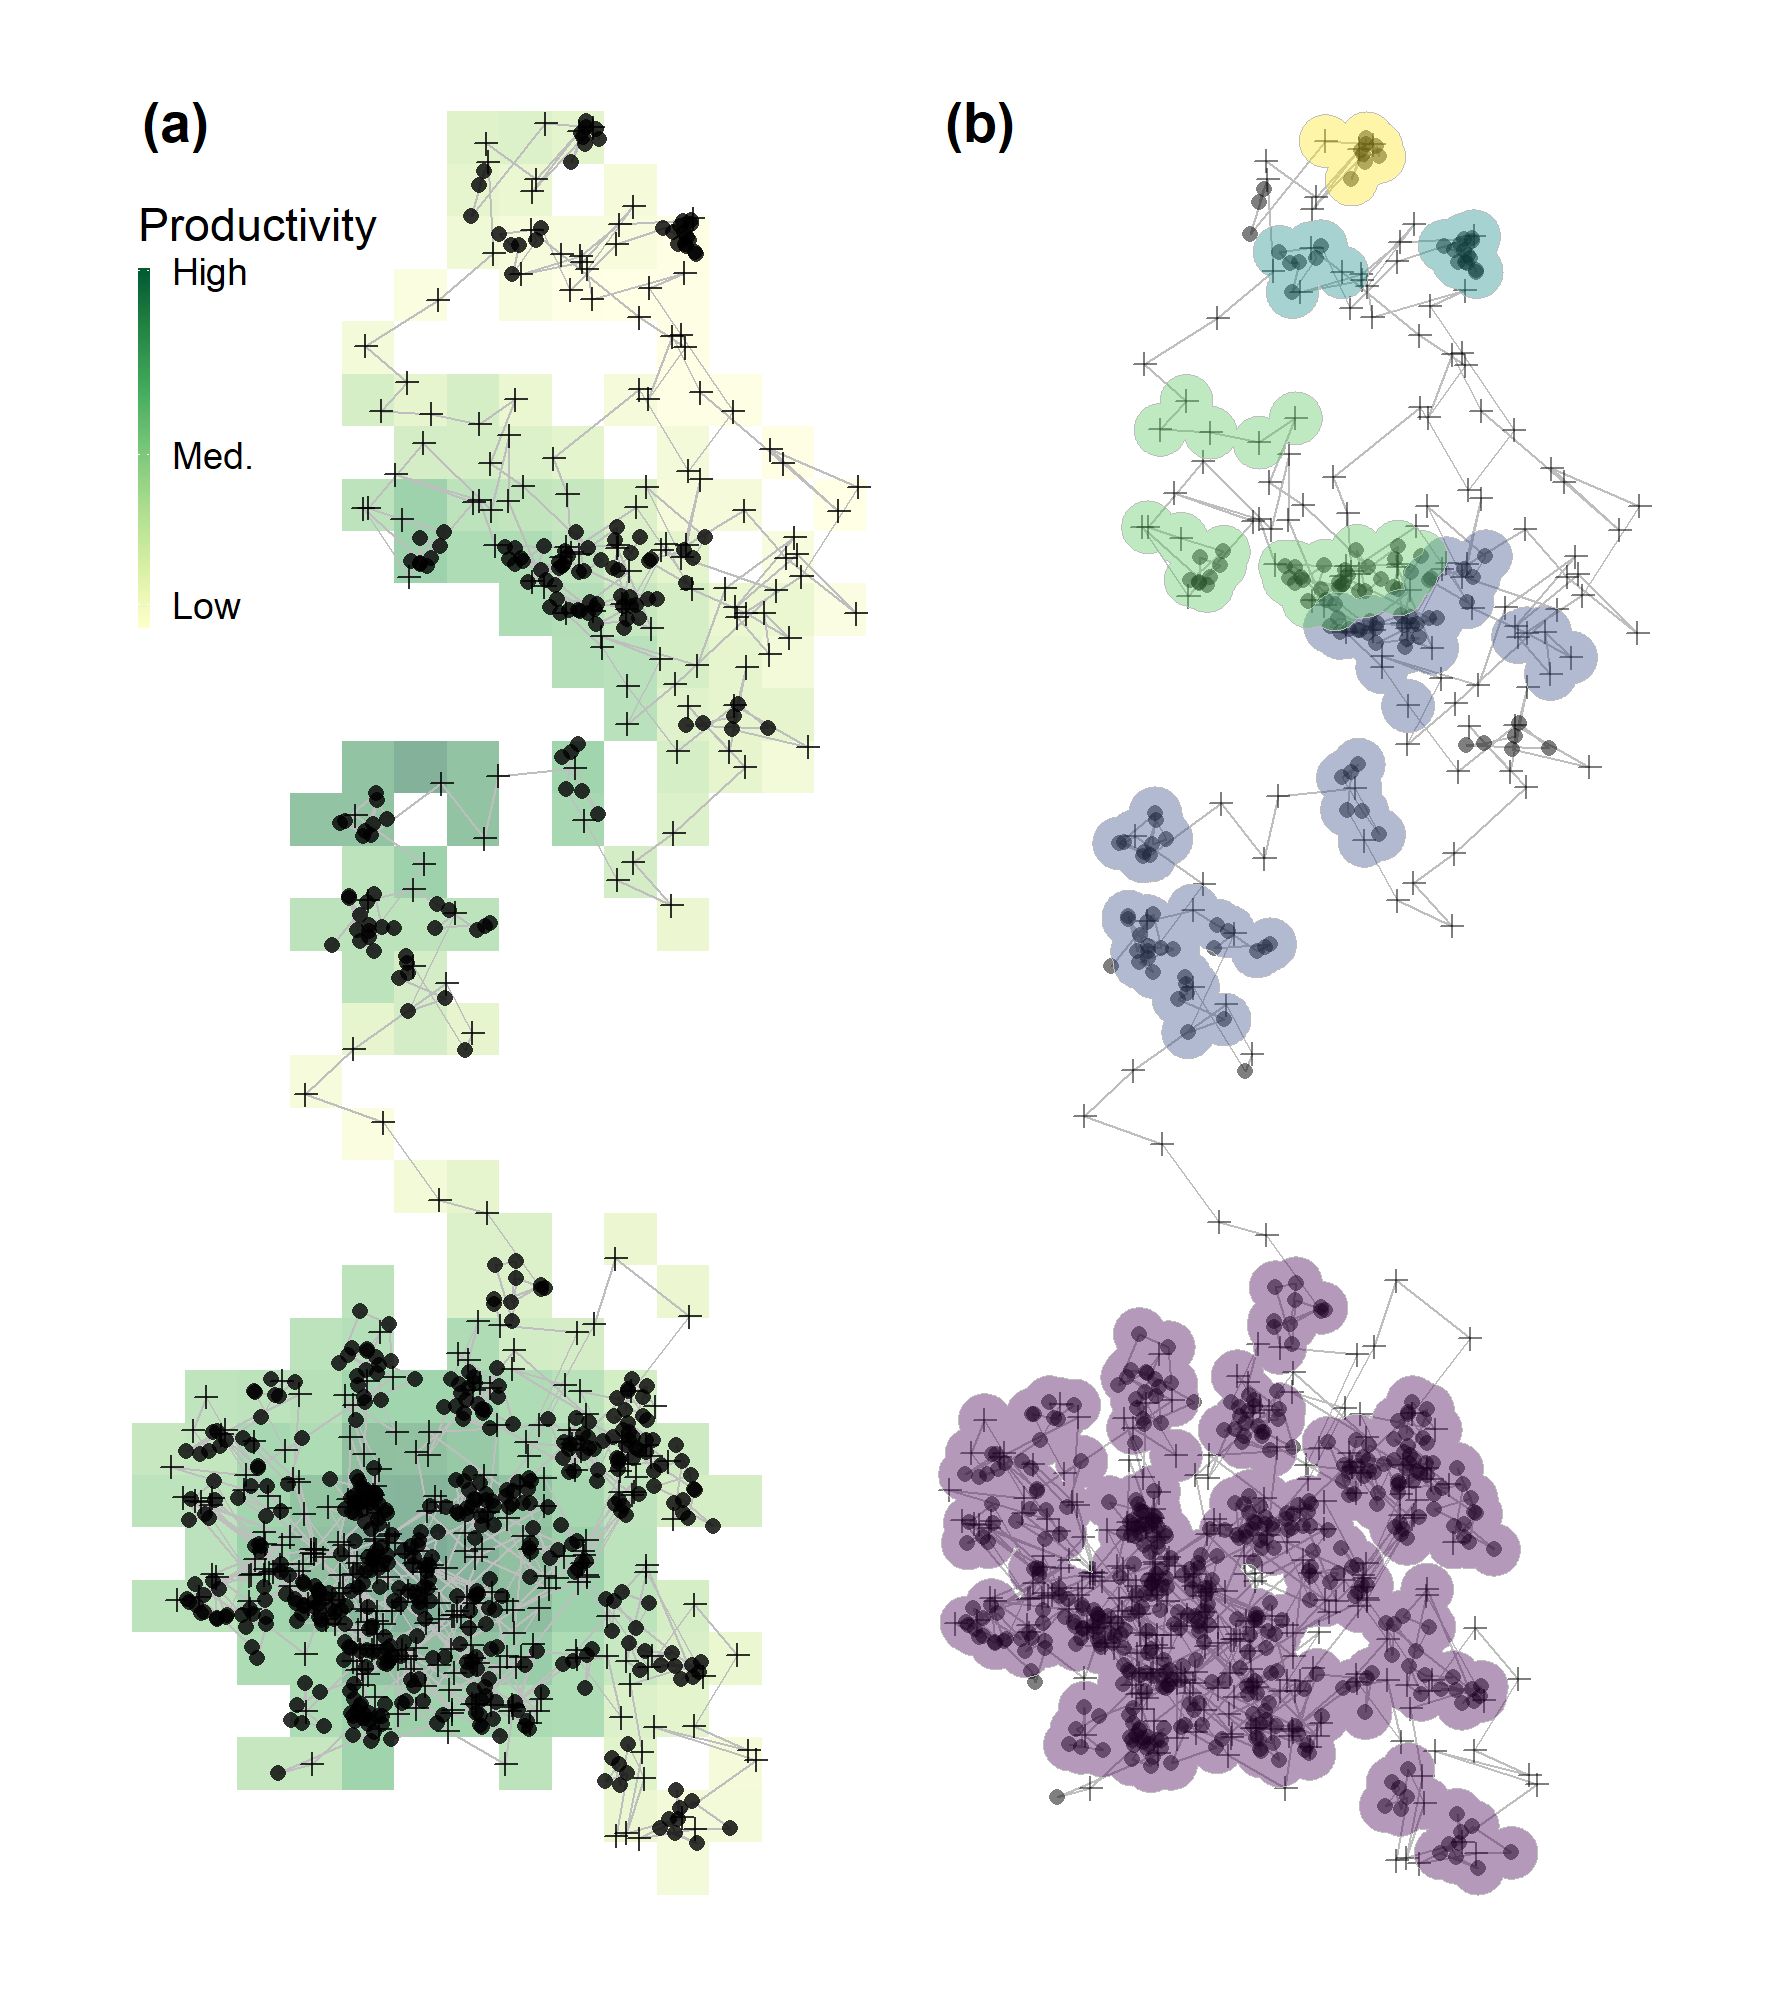
\includegraphics[width=0.75\textwidth]{figures/preprocessing/fig_06.png}
    \caption{
        \textbf{Movement tracks can be classified into residence patches, while leaving out the transit between them.}
        \textbf{(a)} A simulated animal movement track from \citealt{gupte2021a}, where an agent uses local cues to make movement decisions to maximise intake.
        The agent tends to stop (solid circles) on high-productivity areas of the landscape, as these are more likely to generate prey-items.
        Transit points between stationary phases are shown as crosses.
        \textbf{(b)} Our simple, first-principles based clustering algorithm classifies the track into five residence patches. 
        Some transit points are erroneously classified as being part of a residence patch (top, yellow), illustrating why is it important to remove such data before applying this method.
        Simultaneously, some points where the animal is not stationary for long are not picked up by the method.
        While the large purple patch (bottom) is composed almost entirely of consecutive positions, the subsequent patches are composed of multiple parts.
        This is because our method was designed to be robust to missing data from empirical tracks; the spatial and temporal limits of splitting and lumping can be controlled using the arguments passed to \textit{atl\_res\_patch}, and can be adjusted to fit the study system.
        Users are cautioned that there are no `correct' options, and the best guide is the behavioural biology of the tracked individual.
    }
    \label{preproc_fig_06}
\end{figure}

\subsection*{A Real-World Test of User-Built Pre-Processing Tools}

We applied the pre-processing pipeline using \textit{atlastools} functions described above to an ATLAS dataset to verify that the residence patch method could correctly identify known stopping points (see Fig.~\ref{preproc_fig_07}).
We collected the data (n = 50,816) on foot and by boat, with a hand-held WATLAS tag (sampling interval = 1s) around the island of Griend (53.25$^{\circ}$N, 5.25$^{\circ}$E) in August 2020 \citep[WATLAS: Wadden Sea ATLAS system][]{beardsworth2022mee,bijleveld2021}.
Since the data were intended to test the accuracy of the WATLAS system, we were able to log stops in the track as waypoints using a handheld GPS device, and manually annotate the WATLAS data with the timestamp of each waypoint (Garmin Dakota 10; see \citealt{beardsworth2022mee}).
We estimated the real duration of each stop as the time difference between the first and last position recorded within 50m of each waypoint, within a 10 minute window before and after the waypoint timestamp (to avoid biased durations from revisits).
Stops had a median duration of 10.28 minutes (range: 1.75 minutes -- 20 minutes; see Supplementary Material).
We cleaned the data before constructing residence patches by (i) removing a single outlier ($>$ 15 km away), removing unrealistic movement ($\geq$ 15 m/s), smoothing the data ($K$ = 5), and (iv) thinning the data by subsampling over a 30 second interval.
The cleaning steps retained 37,324 positions (74.45\%), while thinning reduced these to 1,803 positions (4.8\% positions of the smoothed track).
Details and code are provided in the Supplementary Material (see \textit{Validating the Residence Patch Method with Calibration Data}).

We began by visualising the data to check for location errors, and found a single outlier position approx. 15km away from the study area (Fig.~\ref{preproc_fig_07}.a).
This outlier was removed by filtering data by the X coordinate bounds using the function \textit{atl\_filter\_bounds}; X coordinate bounds $\leq$ 645,000 in the UTM 31N coordinate reference system were removed (n = 1; remaining positions = 50,815).
We then calculated the incoming and outgoing speed, as well as the turning angle at each position using the functions \textit{atl\_get\_speed} and \textit{atl\_turning\_angle} respectively, as a precursor to targeting large-scale location errors in the form of point outliers.
We used the function \textit{atl\_filter\_covariates} to remove positions with incoming and outgoing speeds $\geq$ the speed threshold of 15 m/s (n = 13,491, 26.5\%; remaining positions = 37,324, 73.5\%; Fig.~\ref{preproc_fig_07}.b).
This speed threshold was chosen as 5 m/s faster than the known boat speed, 10 m/s.
Finally, we targeted small-scale location errors by applying a median smooth with a moving window size $K$ = 5 using the function \textit{atl\_median\_smooth} (Fig.~\ref{preproc_fig_07}.c).
This step does not reduce the number of positions.

We identified stationary positions as those where the median smoothed speed ($K$ = 5) was $<$ 2m/s, as people or a boat moving any faster are likely to be in transit.
We clustered these positions into residence patches with a buffer radius of 5m, spatial independence limit of 50m, temporal independence limit of 5 minutes, and a minimum of 3 positions per patch.
Inferred residence patches corresponded well to the locations of stops (see Fig.~\ref{preproc_fig_07}.c).
However, the residence patch algorithm detected seven more stops (n = 28) than there were waypoints (n waypoints = 21).
One of these was the field station on Griend where the tag was stored between trips (red triangle, Fig.~\ref{preproc_fig_07}.c), while another patch was formed of positions recorded while waiting for the boat; such unintended stops, not recorded as waypoints, likely accounted for the remaining five `extra' residence patches.
Our analysis also did not detect two stops of 105 and 563 seconds (1.75 and 9.4 minutes) since they were data poor and were cleaned away during pre-processing (n positions = 6, 15), highlighting that the quality of the raw data (as in the rest of the track) is still a limiting factor on the inferences that are possible after pre-processing.
To determine whether the residence patch method correctly identified the duration of detected stops in the calibration track, we first extracted the patch attributes using the function \textit{atl\_patch\_summary}.
We then matched the patches to the waypoints by their median coordinates (rounded to 100 metres).
We assigned the inferred duration of the stop as the duration of the spatially matched residence patch.
We compared the inferred duration with the real duration using a linear model with the inferred duration as the only predictor of the real duration.
% We excluded a single waypoint (WP080) since we had accidentally stopped there for $>$ 60 minutes.
Inferred duration was a good predictor of the real duration of a stop (linear model estimate = 1.021, t-value = 12.965, $p <$ 0.0001, $R^2$ = 0.908; see Supplementary Material Fig.~\ref{preproc_fig_01}.7).
This translates to a 2\% underestimation of the stop duration at a tracking interval of 30 seconds.
Finally, any classification algorithm will present users with a trade-off between over-sensitivity (erroneously finding stops where there were none), and under-sensitivity (missing stops where they are not local or long enough) --- users should balance between these based on the broader questions sought to be answered.

% % calibration figure
\begin{figure}[h!]
    \centering
    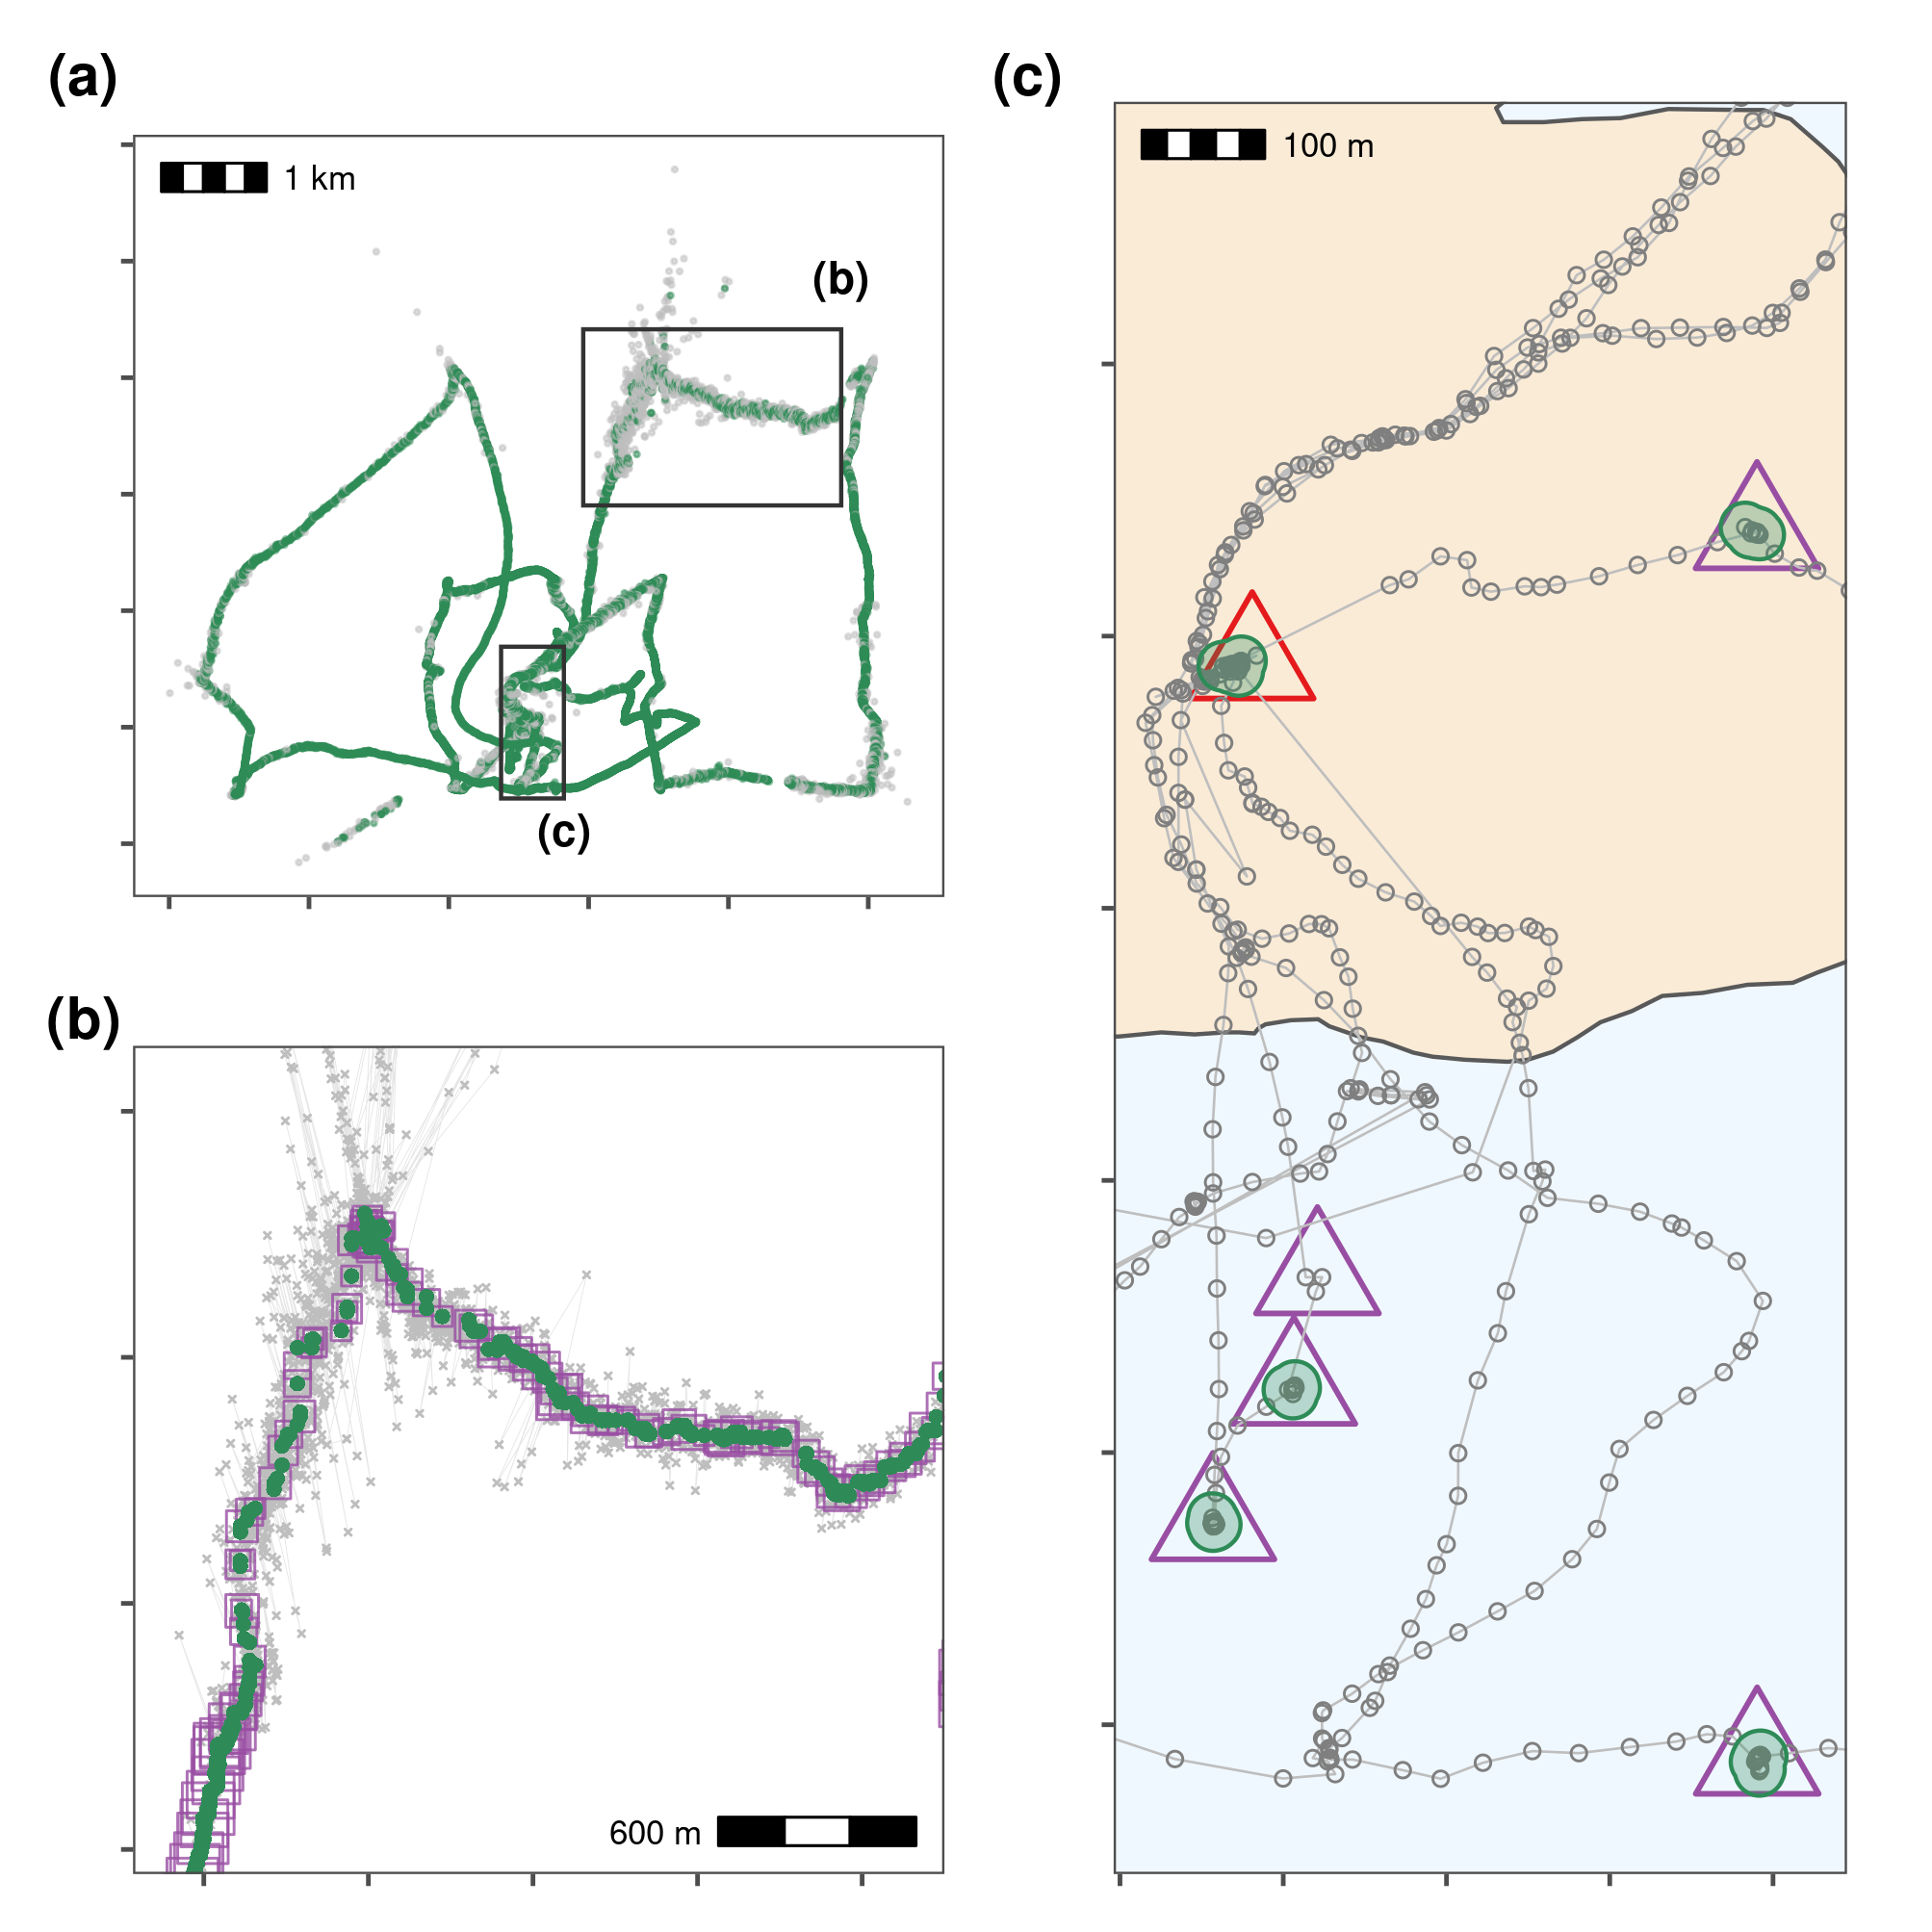
\includegraphics[width=0.75\textwidth]{figures/preprocessing/fig_07.png}
    \caption{
        \textbf{Pre-processing steps for WATLAS calibration data showing filtering on speed, median smoothing and thinning by aggregation, and making residence patches.}
        \textbf{(a)} Positions with incoming and outgoing speed $>$ 15 m/s are removed (grey crosses = removed, green points = retained).
        \textbf{(b)} Raw data (grey crosses), median smoothed positions (green circles; moving window $K$ = 5), and the smoothed track thinned by aggregation to a 30 second interval (purple squares).
        Square size corresponds to the number of positions used to calculate the averaged position during thinning.
        \textbf{(c)} Clustering thinned data into residence patches (green polygons) yields robust estimates of the location of known stops (purple triangles).
        The algorithm identified all areas with prolonged residence, including those which we had not intended to be recorded, such as stops at the field station (n = 12; red triangle).
        Our analysis could not find two stops of 105 and 563 seconds duration (6 and 15 fixes, respectively), since these were lost in the data thinning step; one of these is shown here (purple triangle without green polygon).
    }
    \label{preproc_fig_07}
\end{figure}

\section*{A Worked-Out Example on Animal Tracking Data}

We present a fully worked-out example of our pre-processing pipeline and residence patch method using movement data from three Egyptian fruit bats (\textit{Rousettus aegyptiacus}) tracked using the ATLAS system in the Hula Valley, Israel (33.1$^{\circ}$N, 35.6$^{\circ}$E) (\citealt{toledo2020, lourie2021}).
Code and data can be found in the Supplementary Material and Zenodo repository (see \textit{Processing Egyptian Fruit Bat Tracks}). 
Data selected for this example were collected over three nights (5\textsuperscript{th} -- 7\textsuperscript{th} May, 2018), with an average of 13,370 positions (SD = 2,173; range = 11,195 -- 15,542; interval = 8 seconds) per individual.
Plotting the tracks revealed potential location errors (see Fig.~\ref{preproc_fig_01}, see also Supplementary Material Fig.2.1), which we filtered out by removing observations with ATLAS SD $>$ 20 (see Supplementary Material Section 2.5), as well as removing observations calculated using fewer than four base stations, altogether trimming 22\% of the raw data (mean positions remaining = 10,447 per individual).
% We converted the ATLAS time format (milliseconds since the UNIX Epoch) to the more common UNIX format (seconds since the Epoch) by taking the floored value of the time divided by 1000.
Then, we removed unrealistic movement represented by positions with incoming and outgoing speeds $>$ 20 m/s that exceed the maximum flight speed recorded in this species (15 m/s; \citealt{tsoar2011}), leaving 10,337 positions per individual on average (98\% of previous step).
We median smoothed the data with a moving window $K$ size = 5, and no observations were lost.

We aimed to study bats' night-time foraging on fruit trees by quantifying the duration of bats' residence patches.
We began the construction of residence patches by finding the residence time within 50 metres of each position; this is the maximal radius of a `cloud of points' around fruit trees \citep{bracis2018}.
Foraging bats repeatedly traverse the same routes (\citealt{toledo2020, tsoar2011, lourie2021}) and this could artificially inflate the residence time of positions along these routes.
To avoid confusing revisits with residence, we limited the summation of residence times at each position to the period until the first departure of 5 minutes or more.
Thus, two nearby locations ($\leq$ 50m apart) each visited for one minute at a time, but separated by an interval of some hours would not be clustered together as a residence patch. 
To focus on bats' night-time foraging behaviour, we also excluded positions during the day (5 AM -- 8 PM), and at or near the roost-cave (see Fig.~\ref{preproc_fig_08}a) to focus on night-time foraging behaviour; 22,910 of 31,012 positions remained (73.9\%).
Since bats departed and returned to their roost at different times each night, we also excluded locations with a residence time $>$ 200 minutes (approx. 3.3 hours), as this was more likely to represent daytime roosting than nighttime foraging; of 31,012 smoothed positions, 18,677 remained (60\%).
From these positions, we calculated that between leaving the roost to forage, and returning, bats had a mean residence time at each position of 95.64 minutes (SD = 119.23) --- this value is still likely to be biased by some positions at the roost.

To determine the true duration of foraging, we opted for a first-principles approach and first selected only locations with a residence time $>$ 5 minutes, reasoning that a flying animal stopping for $>$ 5 minutes at a location should plausibly indicate resource use or another interesting localised behaviour.
This step retained 5,736 positions per bat on average (17,208 total), or 72.4\% of the nighttime positions.
We then constructed residence patches with a buffer distance of 25m, a spatial independence limit of 100m, a temporal independence limit of 30 minutes, and rejected patches with fewer than three positions.
These values are meant as examples; users should determine the sensitivity of their results to parameter choices.
Bats spent 56.95 minutes at foraging sites (SD = 62.20), and were stationary in particular fruit trees and roosting trees during 83.8\% of their foraging time (Fig.~\ref{preproc_fig_08}).
Although all three bats roosted at the same cave during the day, and all their tracks are within the typical foraging area of bats roosting in this cave \citep{lourie2021}, they used distinct foraging sites across the area at night (Fig.~\ref{preproc_fig_08}.a). The lack of overlap among individuals in tree use, obtained with the residence patch algorithm, shows that although co-roosting bats share the same cave-specific foraging area \citep{lourie2021}, they often forage on different trees.
Contrasting the actual movement path with the linear path between residence patches can help reveal details of how animal cognition affects space use \citep{toledo2020}.
Bats tended to show prolonged residence near known food sources (fruit trees), but also where no fruit trees were recorded (Fig.~\ref{preproc_fig_08}.b, ~\ref{preproc_fig_08}.c), in line with previous evidence for their use of non-fruiting trees to rest, to handle and digest food, and presumably for social interactions \citep{tsoar2011}.

\begin{figure}[h!]
    \centering
    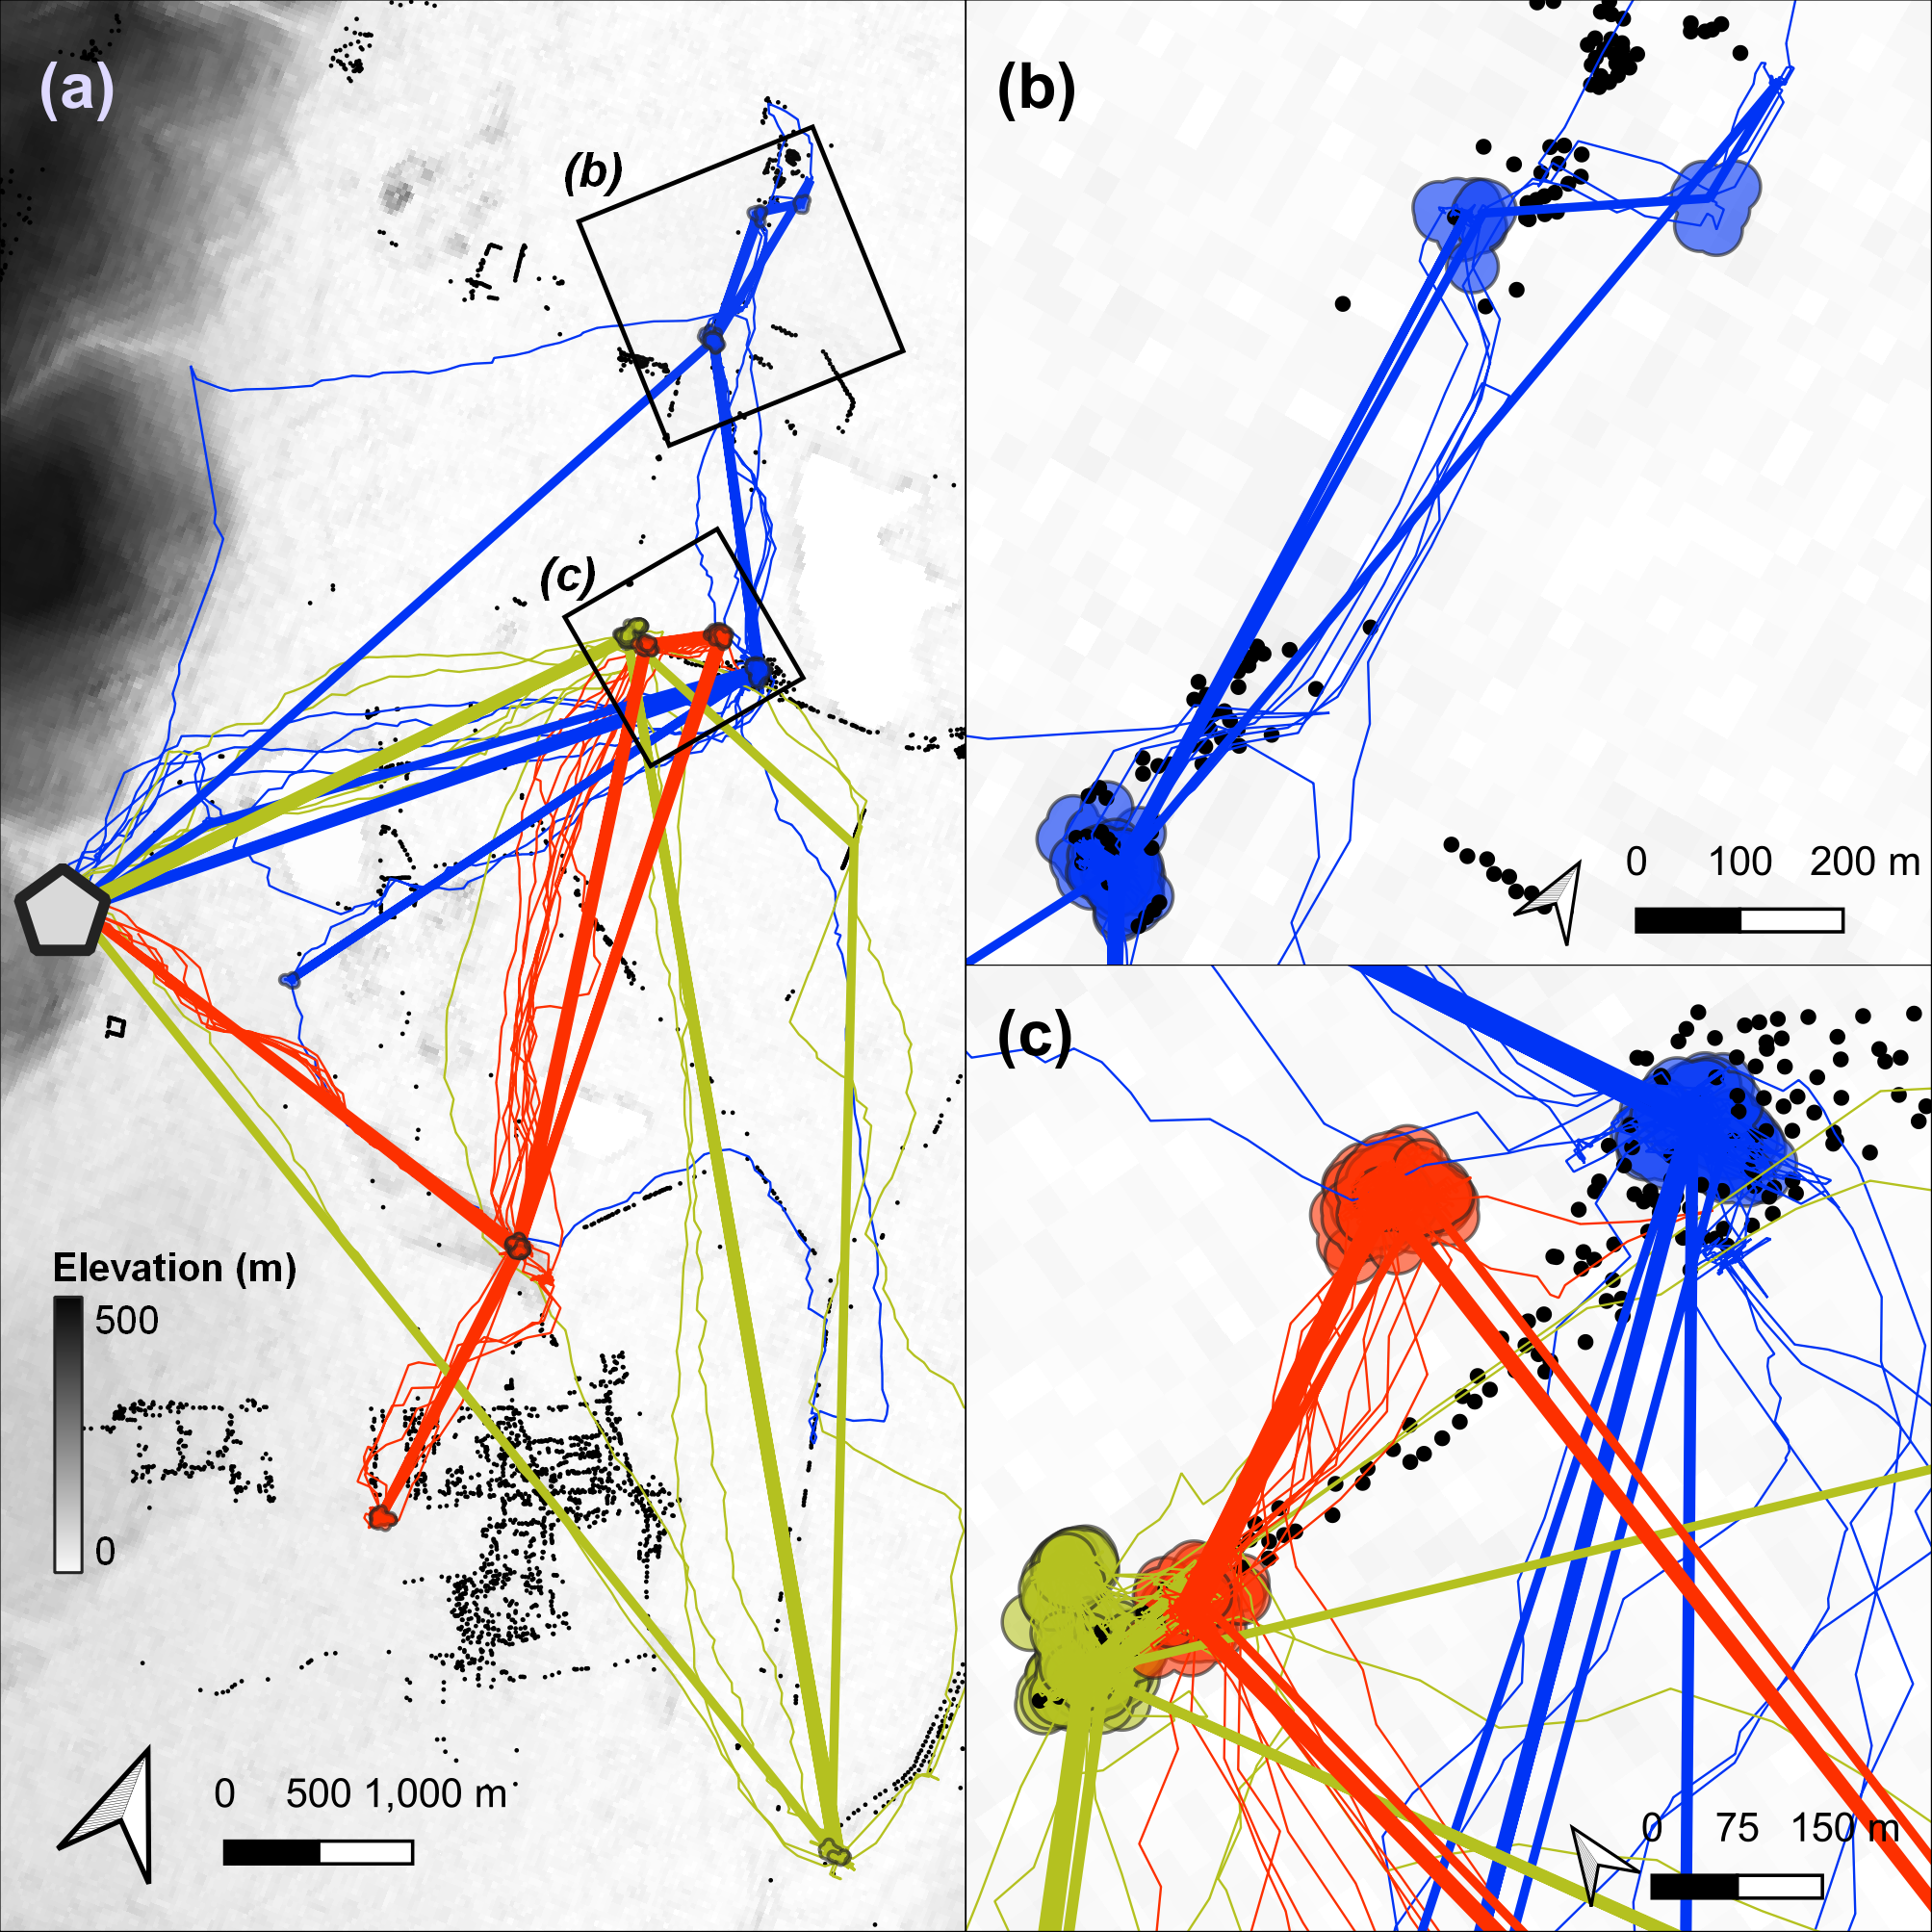
\includegraphics[width=0.75\textwidth]{figures/preprocessing/fig_08.png}
    \caption{
        \textbf{Synthesising animal tracks into residence patches can reveal movement in relation to landscape features, prior exploration, and other individuals.}
        \textbf{(a)} Linear approximations of the paths (coloured straight lines) between residence patches (circles) of three Egyptian fruit bats (\textit{Rousettus aegyptiacus}), tracked over three nights in the Hula Valley, Israel.
        Real bat tracks are are shown as thin lines below the linear approximations, and colours show bat identity. The grey hexagon represents the roost-cave at Gar Hershom.
        Black points represent known fruit trees.
        Background is shaded by elevation at 30 metre resolution.
        \textbf{(b)} Spatial representations of an individual bat's residence patches (green polygons) can be used to study site-fidelity by examining overlaps between patches, or to study resource selection by inspecting overlaps with known resources such as fruit trees (black circles).
        In addition, the linear approximation of movement between patches (straight green lines) can be contrasted with the estimated real path between patches (irregular green lines), for instance, to determine the efficiency of movement between residence patches.
        \textbf{(c)} Fine-scale tracks (thin coloured lines), large-scale movement (thick lines), residence patch polygons, and fruit tree locations show how high-throughput data can be used to study movement across scales.
        Patches and lines are coloured by bat identity.
    }
    \label{preproc_fig_08}
\end{figure}

\section*{Future Perspectives on Pre-processing Tracking Data}

Recent technical advances in wildlife tracking have already yielded exciting new insights from massive high-resolution movement datasets \citep{aspillaga2021, aspillaga2021a, baktoft2017, baktoft2019, harel2016, harel2018, oudman2018, papageorgiou2019, tsoar2011, strandburg-peshkin2015, toledo2020, beardsworth2021a, beardsworth2021b, corl2020, vilk2021, lourie2021}, and high-throughput animal tracking is expected to become increasingly more common in the near future.
Tackling the very large datasets that high-throughput tracking generates requires a different approach from that used for traditionally smaller volumes of data.
We foresee that movement ecologists will have to adopt ever more practices from fields accustomed to dealing with `big data', and that the field will become increasingly computational \citep{peng2011}.

Researchers have long used some of these approaches \textit{ad hoc}, such as exploratory data analysis on small subsets before applying methods to the full data, using efficient tools, and basic batch-processing. 
Yet formally prescribing these steps can help practitioners avoid pitfalls and implement techniques that make their analyses quicker and more reliable.
Standardised principles, implemented a basic pipeline, for approaching data cleaning promote reproducibility across studies, making comparative inferences more robust.
While massive datasets make reliance on standardised pipelines necessary, the output of such pipeline should periodically manually double-checked to ensure `realistic' output.
The open-source \textit{R} package \textit{atlastools} serves as a starting point for methodological collaboration among movement ecologists, and as a simple working example on which researchers may wish to model their own tools.
Efficient location error modelling approaches \citep{fleming2020, aspillaga2021} may eventually make data-cleaning optional.
Yet cleaning tracking data even partially before modelling location error is faster than error-modelling on the full data, and the removal of large location errors may improve model fits.
Thus we see our pipeline as complementary to these approaches \citep{fleming2014, fleming2020}.

Finally, we recognise that the diversity and complexity of animal movement and data collection techniques often requires system-specific, even bespoke, pre-processing solutions.
Though the principles outlined here are readily generalised to numerous data sources (including terrestrial radio-based reverse-GPS: e.g. \citealt{toledo2020}, and marine acoustic reverse-GPS: e.g. \citealt{aspillaga2021}; high-resolution GPS such as \citealt{strandburg-peshkin2015}, and video-tracking: \citealt{rathore2020}), users' requirements will eventually exceed the particular tools we provide.
For instance, relational databases are the standard for storing very large datasets, and extending pre-processing pipelines to deal with various data sources is relatively simple, as we show in our Supplementary Material.
We see the diversity of animal tracking datasets and studies as an incentive for more users to be involved in developing methods for their systems.
We offer our approach to large tracking datasets, and our pipeline and package as a foundation for system-specific tools in the belief that simple, robust concepts are key to methods development that balances system-specificity and broad applicability.\\
{ \begin{center} \barfont{-.-} \end{center} }

%%%%%%%%%%%%% Supplement %%%%%%%%%%%%%%%

% \newpage

\begingroup

\let\clearpage\relax
\let\cleardoublepage\relax
\let\cleardoublepage\relax

{\chapter*{Supplementary Information for Chapter~\ref{ch:preprocessing}}}

The supplementary material for this chapter is a worked out, step-by-step guide to using the \emph{atlastools} package to clean data as described in preceding sections.
Being primarily a tutorial for practitioners --- and quite lengthy --- it is not provided here, but may be found online as Supporting Information published along with the manuscript, \textcite{gupte2022d}, \citetitle{gupte2022d}, at:
https://besjournals.onlinelibrary.wiley.com/doi/10.1111/1365-2656.13610.

{ \begin{center} \barfont{-.-} \end{center} }

\endgroup

%     \newrefcontext[sorting=nyt]
%     \section*{Literature Cited}
%     \printbibliography[title=Literature~Cited,heading=none]
% \end{refsection}


\cleardoublepage %************************************************
\chapter{Individual Consistency in Movement Tendencies Across Spatial Scales}\label{ch:knots}
\chaptermark{Personality \& Movement}
%************************************************

{\noindent \sffamily Selin Ersoy, \textbf{Pratik R. Gupte}, Christine E. Beardsworth, and Allert I. Bijleveld}

\section*{Abstract}

% \graffito{
%     \bigskip

%     {\large{$\Delta$}} Under review at The American Naturalist as Gupte et al. The joint evolution of animal movement and competition strategies.
% }
\small{
    Foraging is essential for many species and understanding factors affect foraging decision is a core topic in ecology.
    Patch-use theory examines how animals make decisions on when to approach and leave a particular foraging patch.
    Even though the individual factors associated with patch movement such as searching and processing the food item or digestive costs were studied under this theory, consistent individual differences (also knows as personalities) were understudied.
    Here we investigated if exploratory personality measured in controlled settings predicts patch movement in the field on red knots.
    We first assayed exploratory tendency of red knots in controlled settings (notably without food) and then release the same birds with transmitters to investigate foraging patch movements in the field.
    We asked how exploration speed in the controlled settings relates to within and between patch movement of an individual during low tide.
    We found that faster exploring red knots visit more patches during low tide and they move faster and stay shorter within the patch.
    The size of the foraging patch did not differ between individuals with different exploratory scores.
    Our findings suggest that exploration measured in captivity predicts exploration in the field, and further provides a framework to study and understand how personality variation may be maintained in populations.

    \noindent {\color{red} WORK IN PROGRESS}
}

\clearpage


\cleardoublepage %************************************************
\chapter{Direct Effects of Wing Moult on the Movement and Habitat Selection of Sub-tropical Birds}\label{ch:holeybirds}
\chaptermark{Wing Moult \& Movement}
%************************************************

{\noindent \sffamily\textbf{Pratik R. Gupte}, Yosef Kiat\textsuperscript{1}, Sivan Toledo\textsuperscript{2}, and Ran Nathan\textsuperscript{3}}

\marginpar{
    \sffamily
    \textsuperscript{1} University of Haifa, Israel.
    
    \medskip
    
    \textsuperscript{2} Tel Aviv University, Israel.
    
    \medskip

    \textsuperscript{3} The Hebrew University of Jerusalem, Israel.
}

\section*{Abstract}

% \marginpar{ 
%     \bigskip

%     {\large{\color{Maroon}$\Delta$}} \normalfont Published in the \textit{Journal of Animal Ecology} as Gupte et al. (2021). A guide to pre-processing high throughput tracking data.
% }

\small{
    The feathered flight of birds requires regular renewal of the wing surface through moult, the process of shedding worn out feathers and growing fresh ones.
    Moult presents birds with the dilemma of needing to move more to acquire resources for feather growth, at precisely the time that their flight capacity is reduced (due to missing wing feathers) and they are vulnerable to predation.
    Despite this central importance of moult to avian ecology, and especially to movement, we know little about its direct effects on the spatial ecology of birds.
    We combined a range of mechanistic approaches to present a first quantification of the direct, short-term effects of wing moult on the movement and habitat selection of four different non-migratory, sub-tropical birds.
    We quantified landscape visibility from a predator viewpoint, and followed the movement of birds in different stages of moult, with a high-throughput position tracking system.
    We found that birds balanced the needs and risks of moult by adjusting their movement to their wing condition.
    Naturally moulting birds moved more than non-moulting birds, but birds with wing feathers experimentally removed moved less.
    Among similarly vegetated areas, birds preferred low-visibility sheltered sites in our agricultural landscape, regardless of their moult status.
    Intriguingly, our results suggest that birds' cognitive abilities may extend to seeing a landscape from the spatial perspective of another individual.   
}

\clearpage



\cleardoublepage %************************************************
\chapter{Land-cover and Climate Shape Bird Occupancy in a Tropical Biodiversity Hotspot}\label{ch:hillybirds}
\chaptermark{Citizen Science \& Bird Distributions}
%************************************************
% Using citizen science to parse climatic and land cover influences on

{\noindent \sffamily Vijay Ramesh\textsuperscript{1}, \textbf{Pratik R. Gupte}, Morgan Tingley\textsuperscript{2}, V.V. Robin\textsuperscript{3}, and Ruth S. de Fries\textsuperscript{1}}

\marginpar{
    \sffamily
    \textsuperscript{1} Columbia University, USA.
    
    \medskip
    
    \textsuperscript{2} University of California --- Los Angeles, USA.
    
    \medskip

    \textsuperscript{3} Indian Institute for Science Education and Research --- Tirupati, India.
}

\section*{Abstract}

\marginpar{ 
    \bigskip

    {\large{\color{Maroon}$\Delta$}} \normalfont Under review at \textit{Ecography} as Ramesh et al. Using citizen science to parse climatic and land cover influences on bird occupancy within a tropical biodiversity hotspot.
}

\small{
    Disentangling associations between species occupancy and its environmental drivers --- climate and land cover --- along tropical mountains is imperative to predict species distributional changes in the future. 
    Previous studies have largely focused on identifying such associations along temperate mountain systems. 
    Using robustly filtered citizen science observations, we examined the role of climatic and landscape variables and its association with species occurrence within a tropical biodiversity hotspot. 
    We used over 1.1 million citizen scientist observations contributed to eBird between 2013 and 2020 for 82 species of birds across the southern Western Ghats in India and modeled the regional distribution of each species within an occupancy modeling framework. 
    Our results show that mean variation in temperature (defined as temperature seasonality), presence of evergreen forests, and presence of deciduous forests were significantly associated with species-specific probabilities of occupancy for 79\% (n=63 birds), 45\% (n=36 birds) and 17\% (n=14 birds) of bird species examined, respectively. 
    Forest specialists were largely sensitive to temperature seasonality and were negatively associated with increasing mean variation in temperature. 
    Human-modified land cover types --- such as the proportion of agriculture/settlements, plantations, and mixed/degraded forests --- were largely negatively associated with the occupancy of forest species, while showing a positive association for many generalist birds. 
    Our study shows that rigorously filtered citizen science observations can be used to identify associations between environmental drivers and species occupancy on tropical mountains. 
    Though current distributions of tropical montane birds of the Western Ghats are strongly driven by climatic factors --- chiefly temperature seasonality --- naturally occurring land cover types including forests are critical to sustain montane avifauna across human-modified landscapes in the long run.
}

\clearpage



% \ctparttext{
%     Mechanistic, individual-based models can capture the complexity and diversity of animal behaviour with spatial contexts --- simultaneously, they can be used to investigate methods used in empirical studies.
    
%     \medskip

%     \textit{Chapter 3} presents a translation of the step-selection paradigm into an individual-based model to study the evolution of movement and competition strategies.
%     Feedbacks between ecology and evolution lead to unexpected outcomes, including substantial individual variation, and the correlation of movement and competition strategies.

%     \medskip

%     \textit{Chapter 4} takes the evolved populations from \textit{Chapter 3} and parses them through the lens of two methods in animal behaviour: repeatability analysis, and step-selection analysis.
%     Applying these methods to scenarios with known mechanisms explains aspects of their performance on real data.
% }
% \part{Mechanistic Modelling and Investigating Empirical Methods}

\cleardoublepage \begin{refsection}
%************************************************
\chapter{The Joint Evolution of Animal Movement and Competition Strategies}\label{ch:kleptomove}
\chaptermark{Competition and Movement}
%************************************************

{\noindent \textbf{Pratik R. Gupte}, Christoph F.G. Netz, and Franz J. Weissing}

\section*{Abstract}

{
    \small
    Competition typically takes place in a spatial context, but eco-evolutionary models rarely address the joint evolution of movement and competition strategies.
    Here we investigate a spatially explicit forager-kleptoparasite model where consumers can either forage on a heterogeneous resource landscape, or steal resource items from conspecifics (kleptoparasitism). We consider three scenarios: (1) foragers without kleptoparasites; (2) consumers specializing as foragers or as kleptoparasites; and (3) consumers that can switch between foraging and kleptoparasitism depending on local conditions.
    We model movement strategies as individual-specific combinations of preferences for environmental cues, similar to step-selection coefficients.
    Using mechanistic, individual-based simulations, we study the joint evolution of movement and competition strategies, and we investigate the implications for the distribution of consumers over this landscape.
    Movement and competition strategies evolve rapidly and consistently across scenarios, with marked differences among scenarios, leading to differences in resource exploitation patterns.
    In scenario 1, foragers evolve considerable individual variation in movement strategies, while in scenario 2, movement strategy shows a swift divergence between foragers and kleptoparasites.
    When individuals' competition strategy is conditional on local cues, movement strategies facilitate kleptoparasitism, and individual consistency in competition strategy also emerges.
    Across scenarios, the distribution of consumers differs substantially from `ideal free' predictions.
    This is related to the intrinsic difficulty of moving effectively on a depleted resource landscape with few reliable movement cues.
    Our study emphasises the advantages of a mechanistic approach when studying competition in a spatial context, and suggests how evolutionary modelling can be integrated with current work in animal movement ecology.

    \bigskip

    {\noindent \large{$\Delta$}} Under review at \textit{The American Naturalist} as Gupte et al. \citetitle{gupte2021a}.
}

% \subsection*{Data and Code}
% {
%     \small
%     Simulation model: github.com/pratikunterwegs/Kleptomove.\\ %and Zenodo: zenodo.org/record/4905476. 
%     \noindent Simulation data (DataverseNL): doi.org/10.34894/JFSC41.\\
%     \noindent Data analysis code: github.com/pratikunterwegs/klepto-move-evol.% and on Zenodo: doi.org/10.5281/zenodo.4904497.
% }

\clearpage

\cleardoublepage 
\newrefcontext[sorting=ynt]

\lettrine{I}{ntraspecific} competition is an important driver of population dynamics and the spatial distribution of organisms \parencite{krebs1978}, and has two main types, `exploitation' and `interference'.
In exploitation competition, individuals compete indirectly by depleting a common resource, while in interference competition, individuals compete directly by interacting with each other \parencite{birch1957,case1974,keddy2001}.
A special case of interference competition which is widespread among animal taxa is `kleptoparasitism', in which an individual steals a resource from its owner \parencite{iyengar2008}.
Since competition has an obvious spatial context, animals should account for the locations of competitors when deciding where to move \parencite{nathan2008a}.
This is expected to have downstream effects on animal distributions across spatial scales, from resource patches \parencite{fretwell1970}, to species distributions \parencite{duckworth2007,schlagel2020}.
Animal movement strategies are thus likely to be adaptive responses to landscapes of competition, with competitive strategies themselves being evolved responses to animal distributions.
Empirical studies of this joint evolution are nearly impossible at large spatio-temporal scales.
This makes models linking individual movement and competition strategies with population distributions necessary.

Contemporary individual-to-population models of animal space-use \parencite[reviewed in][]{deangelis2019} and competition, however, are only sufficient to represent very simple movement and prey-choice decisions.
% \graffito{
%     These classical foraging models correspond to real conditions as much as macro-economic models do with the real world.
%     They are likely useful only at very broad scales.
% }
For example, models including the ideal free distribution \parencite[IFD;][]{fretwell1970}, information-sharing models \parencite[][]{giraldeau1999,folmer2012}, and producer-scrounger models \parencite[][]{barnard1981,vickery1991,beauchamp2008}, often treat foraging competition in highly simplified ways.
Most IFD models consider resource depletion unimportant or negligible \parencite[continuous input models, see][]{tregenza1995, vandermeer1997}, make simplifying assumptions about interference competition, or even model an \textit{ad hoc} benefit of grouping \parencite[e.g.][]{amano2006b}.
Meanwhile, producer-scrounger models primarily examine the benefits of choosing either a producer or scrounger strategy given local conditions, such as conspecific density \parencite{vickery1991}, or the order of arrival on a patch \parencite{beauchamp2008}.
Overall, these models simplify the mechanisms by which competition decisions are made, and downplay spatial structure \parencite[see also][]{holmgren1995, garay2020, spencer2018}.

On the contrary, spatial structure is key to foraging (competition) decisions \parencite{beauchamp2008}.
How animals are assumed to integrate the costs (and potential benefits) of competition into their movement decisions has important consequences for theoretical expectations of population distributions \parencite{vandermeer1997,hamilton2002,beauchamp2008}.
In addition to short-term, ecological effects, competition also likely has evolutionary consequences for individual \textit{movement strategies}, setting up feedback loops between ecology and evolution.
Modelling competition and movement decisions jointly is thus a major challenge.
Some models take an entirely ecological view, assuming that individuals move or compete ideally, or according to fixed strategies \parencite{vickery1991,holmgren1995,tregenza1995,amano2006b}, but see \parencite{hamilton2002}.
Models that include evolutionary dynamics in movement \parencite{dejager2011,dejager2020} and foraging competition strategies \parencite{beauchamp2008,tania2012} are more plausible, but they too make arbitrary assumptions about the functional importance of environmental cues to individual decisions.

Mechanistic, individual-based models are well suited to capturing the complexities of spatial structure, animal decision-making, and evolutionary dynamics \parencite{guttal2010,kuijper2012,getz2015,getz2016,white2018,long2020,netz2021}; for conceptual underpinnings see \textcite{huston1988,mueller2011,deangelis2019}.
% \graffito{
%     I've been lucky enough to have been taught by, or to have met, many of these authors, including Vishu Guttal, Iain Couzin, Wayne Getz, Thomas M\"uller, and Don DeAngelis.
% }
% \graffito{
%     Reading Lauren White's implementation of movement decisions as resource selection functions \parencite{white2018} was instrumental in how I thought about my work.
%     Her model also inspired Chapter~\ref{ch:pathomove}.
% }
Individual-based models can incorporate the often significant variation in movement and competition preferences found in populations, allowing individuals to make different decisions given similar cues \parencite[][]{laskowski2013}.
Individual-based models also force researchers to be explicit about their modelling assumptions, such as \textit{how exactly} competition affects fitness.
Similarly, rather than taking a purely ecological approach and assuming individual differences \parencite[e.g. in movement rules:][]{white2018}, allowing movement strategies to evolve in a competitive landscape can reveal whether individual variation emerges in plausible ecological scenarios \parencite[as in][]{getz2015}.
This allows the functional importance of environmental cues for movement \parencite[see e.g.][]{scherer2020} and competition decisions in evolutionary models to be joint outcomes of selection, and lets different competition strategies to be associated with different movement strategies \parencite[][]{getz2015}.

Here, we present a spatially-explicit, mechanistic, individual-based model of intraspecific foraging competition, where movement and competition strategies jointly evolve on a resource landscape with discrete, depletable food items that need to be processed (`handled') before consumption.
% \graffito{
%     The Kleptomove model's source code is adapted from an earlier predator-prey model
%     \parencite{netz2021}.
% }
In our model, foragers make movement decisions using inherited, evolvable preferences for local ecological cues, such as resource and competitor densities; the combination of preferences for each cue forms individuals' movement strategy \parencite[similar to relative step-selection:][]{fortin2005, avgar2016}.
Lifetime resource consumption is our proxy for fitness; more successful individuals produce more offspring, transmitting their movement and foraging strategies to future generations (with small mutations).
We consider three scenarios: in the first scenario, we examine only exploitation competition.
In the second scenario, we introduce kleptoparasitic interference as an inherited strategy, fixed through an individual's life.
In the third scenario, we model kleptoparasitism as a behavioural strategy conditioned on local environmental and social cues; the mechanism underlying this foraging choice is also inherited.

Our model allows us to examine the evolution of individual movement strategies, population-level resource intake, and the spatial structure of the resource landscape.
The model enables us to take ecological snapshots of consumer-resource dynamics (animal distributions, resource depletion, and competition) proceeding at evolutionary time-scales.
Studying these snapshots allows us to check whether, when, and to what extent the spatial distribution of competitors resulting from the co-evolution of competition and movement strategies corresponds to standard IFD predictions.
We investigate \textit{(1)} which movement strategies evolve in our three competition scenarios, \textit{(2)} whether movement strategies differ within and between competition strategies in our scenarios, and \textit{(3)} whether the emergent spatial distributions of consumers corresponds to `ideal free' expectations.

\section*{The Model}

Individual-based models have to explicitly specify numerous assumptions (e.g. spatial structure, individual interactions, event timescales), but this helps expose assumptions that are often hidden below the surface in analytical models. 
We kept our model assumptions as simple and generic as possible, striving for general, conceptual insights.
To keep the model realistic, we based it on the foraging behavior of shorebirds such as oystercatchers (\textit{Haematopus} spp.), which are extensively studied in the context of foraging competition, both empirically \parencite[e.g.][]{vahl2005, vahl2005a,vahl2007a, rutten2010, rutten2010a}, and using individual-based models \parencite[reviewed in][]{stillman2010}.

% \graffito{
%     We initially tried 100 timesteps, but settled on 400 as this allowed enough time for individuals' intake to be a function of their movement strategy, rather than their good fortune in being initialised in a productive part of the landscape.
% }
Our environment is a fine grid of cells, and each grid cell can hold multiple individuals.
Resources are discrete, as is our conception of time within and between generations. 
Our population, with a fixed number of individuals (N = 10,000), moves on a landscape of 512\textsuperscript{2} grid cells (approx. 1 individual per 26 cells), with wrapped boundaries (i.e., a torus); individuals passing beyond the bounds at one end re-appear on the opposite side.
The model has two time scales, first, an ecological time scale of $T$ timesteps comprising one generation (default $T$ = 400), during which individuals move, make foraging decisions, and handle prey-items they find or steal.
Individuals are immobile while handling food items, creating the conditions for kleptoparasitism \parencite{brockmann1979,ruxton1992}.
At the end of each generation, individuals reproduce, transmitting their movement and foraging strategies to their offspring, whose number is proportional to individual intake at the ecological time scale.
Our model has 1,000 generations, and this comprises the evolutionary timescale.

\subsection*{Resource Landscape}

\paragraph{Prey Abundance}

% \graffito{
%     Early versions of this model had one giant resource peak; this was dropped as it was relatively easy for individuals to find their way to productive areas.
% }
We considered our discrete resources, called `prey-items' to represent mussels, a common prey of many shorebirds, whose abundances are largely driven by external gradients.
We assigned each cell a constant probability of generating a new prey-item per timestep, which we refer to as the cell-specific growth rate $r$.
We modelled clustering in landscape productivity by having the distribution of $r$ across the grid take the form of 1,024 resource peaks, placed at regular distances of 16 grid cells from the peaks around them; $r$ declines from the centre of each peak (called $r_{max}$) to its periphery (see Fig.~\ref{klepto_fig_01}A).
Thus the central cell generates prey-items five times more frequently than peripheral cell: at $r_{max}$ = 0.01, central cells generate one item per 100 timesteps (four items/generation), while the peripheral cells generate one item only every 500 timesteps ($<$ one item/generation).
All landscape cells have a uniform carrying capacity $K$ of 5 prey-items.
While a cell is at carrying capacity its $r$ is 0.
Cells are initialised with prey-items proportional to their $r$ (see e.g. Fig.~\ref{klepto_fig_01}A).

\paragraph{Prey Acquisition by Foragers}

Foragers perceive a cue indicating the number of prey-items $P$ in a cell, but fail to detect each item with a probability $q$, and are thus successful in finding a prey-item with a probability $1 - q^P$.
Individuals on a cell forage in a randomised sequence, and the probability of finding a prey-item ($1 - q^P$) is updated as individuals find prey, reducing $P$.
Foragers that find a prey-item must handle it for a fixed handling time $T_H$ (default = 5 timesteps), before consuming it \parencite[][]{ruxton1992}.
Natural examples include the time required for an oystercatcher to break through a mussel shell, or a raptor to subdue prey; overall, the handling action is obvious, and the prey is not fully under the control of the finder \parencite{brockmann1979}.
Foragers that do not find a prey-item are considered idle in that timestep, and are counted as `non-handlers'.
Similarly, handlers that finish processing their prey in timestep $t$ can only forage again in timestep $t+1$, i.e., they are idle in the timestep $t$.

\subsection*{Movement Strategies}

All individuals move simultaneously at the end of each timestep $t$, and then implement their foraging or kleptoparasitic behaviour to acquire prey.
However, handlers do not make any movements until they have fully handled and consumed their prey.
We model movement as comprised of small, discrete steps between adjacent cells.
Across scenarios, individuals make movement decisions using evolved cue preferences.
Individuals select a destination cell, after assessing potential destinations based on available cues, similar to approaches used previously \parencite{getz2015,getz2016,white2018,scherer2020,netz2021}.

% \graffito{
%     Our individuals can use much more complex functions, encoded by neural networks, an idea that has been explored, but not widely used, in movement ecology \parencite{mueller2011}.
% }
To move, individuals scan the nine cells of their Moore neighbourhood for three environmental cues, \textit{(1)} an indication of the number of discrete prey-items $P$, \textit{(2)} the number of individuals handling prey $H$ (`handlers'), and \textit{(3)} the number of individuals not handling prey $N$ (`non-handlers').
Individuals rank the potential destinations (including their current cell) by their suitability $S$, where $S = s_PP + s_HH + s_NN$, and move to the most suitable cell in timestep $t+1$.
The individual preferences for each cue, $s_P$, $s_H$, and $s_N$, have numeric values, are considered to be evolvable traits that can be transmitted between generations, and undergo independent mutation.
Since individuals are constrained to perceiving and moving short distances, they may not always sense their best long-term move.

It is the combination of cue preferences, and especially their value relative to each other, that determines individual movement decisions \parencite[similar to relative selection coefficients,][]{fortin2005,avgar2016,white2018}. 
For example, an extreme value of $s_P$ relative to the other preferences would mean that an individual's movement decisions are guided primarily by differences in the local density of prey-items.
We call an individual's combination of inherited preferences its \textit{movement strategy} (see e.g. Fig.~\ref{klepto_fig_01}E).

\subsection*{Competition Strategies}

\paragraph{Scenario 1: Exploitative Competition}

In scenario 1, we simulate only exploitative competition; individuals (henceforth called `foragers') move about on the landscape and probabilistically find, handle, and consume prey-items.
Foragers can be either in a `searching' or a `handling' state \parencite{holmgren1995}.

\paragraph{Scenario 2: Foraging or Kleptoparasitism as Fixed Strategies}

% \graffito{
%     The Kleptomove simulation can be modified to change the probability of kleptoparasite success.
% }
In scenario 2, the competition strategy is genetically determined and transmitted from parents to offspring: exploitative competition (by foragers), or kleptoparasitic interference (by kleptoparasites).
Kleptoparasites cannot extract prey-items directly from the landscape, and only steal from handlers \parencite[see][]{holmgren1995}.
Kleptoparasites are always successful in stealing from handlers, and such successful surprise attacks are commonly observed among birds \parencite{brockmann1979}.
When multiple kleptoparasites target the same handler, only one (randomly selected) is considered successful --- thus kleptoparasites compete exploitatively among themselves.
Kleptoparasites displace the handler that they robbed of prey up to 5 cells away from their location.
Having acquired prey, kleptoparasites become handlers, but need only handle prey for $T_H - t_h$ timesteps, where $t_h$ is the time that the prey has already been handled by its previous owner.
Once a kleptoparasite becomes a handler, it can also be targeted by other kleptoparasites.
Unsuccessful kleptoparasites are considered idle, and are counted as non-handlers.
Movement strategies evolve independently of the competition strategy, as in scenario 1; however, the optimal movement strategy for foragers need not be the same as that for kleptoparasites.

\paragraph{Scenario 3: Conditional Interference Competition}

% \graffito{
%     Similar to movement decisions, competition decisions can also be encoded by a neural network.
% }
In scenario 3, each individual can either act as a forager, or as a kleptoparasite, depending on its assessment of local conditions.
Similar to how movement decisions are made based on local cues, individuals process cell-specific environmental cues in timestep $t$ to determine their competition strategy in the next timestep as
% \begin{linenomath*}
\begin{equation}
    \text{strategy} = 
\begin{cases}
    \text{forager},& \text{if } w_PP + w_HH + w_NN \geq w_0\\
    \text{kleptoparasite},              & \text{otherwise}
\end{cases}
\end{equation}  
% \end{linenomath*}
where the cue preferences $w_P$, $w_H$ and $w_N$, and the threshold value $w_0$, are numeric values, and heritable between generations (with small, rare, independent mutations).
The combination of the cue preferences for competition decisions forms each individual's \textit{competition strategy}.
Individuals' competition strategies may lead to specialisation as foragers or kleptoparasites (as in scenario 2), or to plastic behaviour conditioned on local cues.
The competition dynamics are the same as in scenario 2.

\subsection*{Reproduction and Inheritance}

Our model considers a population of fixed size (10,000 individuals) with discrete, non-overlapping generations. 
For simplicity, we assume that individuals are haploid and reproduction is asexual. 
In scenarios 1 and 2, individuals only inherit and transmit their cue preferences ($s_P$, $s_H$, $s_N$) which determine movement decisions.
In scenario 3, individuals also inherit cue preferences for competition decisions ($w_P$, $w_H$, $w_N$, $w_0$), and transmit them to offspring.
The movement and competition cue preferences all mutate independently in scenario 3.
% \graffito{
%     The implicit assumption here is fecundity effects, rather than mortality effects. This is consistent with many shorebirds, which often fail to breed in bad years, but have very high adult survival.
% }
Each individual's number of offspring is proportional to the individual's total lifetime intake of resources; hence, resource intake is used as a proxy for fitness. 
A weighted lottery (with weights proportional to lifetime resource intake) selects a parent for each offspring in the subsequent generation \parencite[see e.g.][]{tania2012,netz2021}.
Across scenarios, the cue preferences for movement decisions are subject to rare, independent mutations ($\mu$ = 0.001).
The mutational step size (either positive or negative) is drawn from a Cauchy distribution with a scale of 0.01 centred on zero, allowing for a small number of very large mutations while most mutations are small.
In scenario 2, foragers may infrequently mutate into a kleptoparasite (or \textit{vice versa}; $\mu$ = 0.001).
In scenario 3, the competition cue preferences also mutate as described above.
Each offspring is initialised at random locations on the landscape, leading individuals to experience conditions potentially different from those of their parent.
We chose this option because it allows us to focus on adaptive movement strategies, whereas limited dispersal confounds movement and local adaptation.

\subsection*{Simulation Output and Analysis}

% \graffito{
%     The simulation output, in a Windows-specific compressed format, required a number of specialised functions to extract useful information.
% }
We ran all three scenarios at a default $r_{max}$ of 0.01, which we present in the \textsc{Results}, and also across a range of $r_{max}$ values between 0.001 and 0.05 (see Fig.~\ref{klepto_fig_06} and Supplementary Material Figs. 7 -- 9).
We initialised the cue preferences with values drawn from a Cauchy distribution with a scale of 0.01 centred on zero; this allows a very small amount of variation in the population (see e.g. Fig.~\ref{klepto_fig_01}E), and is equivalent to a single generation of mutation from all preferences initialised at zero (see \textsc{Reproduction and Inheritance} above).
Normalising each individual's cue preferences by the sum of the absolute values of all preferences $s_I = s_I / (|s_P| + |s_H| + |s_N|)$, for $s_I \in s_P, s_H, s_N$, makes it possible to visualise individuals on a three-dimensional trait space of relative preferences bounded by (-1.0: \textit{strongly avoid}, +1.0: \textit{strongly prefer}).
With remarkably consistent outcomes across replicates in each scenario, and as each simulation run produced massive datasets, we show the outcomes of three replicates here.
More data can be generated and analysed using the code linked below.

\paragraph{Population Activities and Intake}

Across scenarios, in each generation, we counted the number of times foragers were searching for prey, kleptoparasites were searching for handlers, and the number of timesteps that individuals of either strategy were handling a prey-item.
We refer to the ratio of these values as the population's `activity budget'.
We examined how the population activity budget developed over evolutionary time, and whether a stable equilibrium was reached.
Furthermore, we counted the population's mean per-capita intake per generation as a measure of population productivity.

\paragraph{Visualising Movement Strategies}

To understand the evolution of individual movement and competition strategies, we exported the cue preferences of each individual in every generation of the simulation.
We scaled each cue preference by the sum of the absolute values of the preferences, allowing us to plot individuals in a standardised three-dimensional trait space of relative cue preferences (with colour as an axis on a two-dimensional plot).
Individuals' position in this space allowed us to easily visualise and compare variation in movement strategies within and between competition strategies and across scenarios.

\paragraph{Visualising Scenario 3 Competition Strategies}

Scenario 3 competition strategies are determined by four values (3 preferences and threshold value), and competition decisions are outcomes of the interactions of these preferences with individuals' movement decisions and ecological conditions.
This makes strategies \textit{per se} difficult to visualise.
We first scaled the competition cue preferences and the threshold value as we did the movement cue preferences.
To illustrate variation in the competition strategies evolved, we presented each individual in representative generations (G = 10, 30, 100, 300, 950) with combinations of two key cues, handler and prey density (each 0 -- 5; 36 combinations overall).
We summarised the proportion of individuals that would attempt to steal at each combination of cue values (see Eqn. 1; Fig.~\ref{klepto_fig_04}F).

\paragraph{Ecological Snapshots of Consumer-Resource Distributions}

We exported snapshots of the entire simulation landscape at the mid-point of each generation ($t$ = 200).
Each snapshot contained data on \textit{(1)} the number of prey-items, \textit{(2)} the number of handling individuals, and the number of individuals using either a \textit{(3)} searching forager strategy or \textit{(4)} kleptoparasitic strategy, on each cell.
We used a subset of the total landscape (60\textsuperscript{2} of 512\textsuperscript{2} cells) for further analyses to speed up computation.
We determined the availability of direct resource cues for movement in each cell by calculating the cell-specific item gradient for each landscape snapshot, as the difference in prey counts between each cell and its neighbouring cells.
For each generation, we calculated the proportion of cells from which it was possible to sense differences in prey-items, i.e., a neighbouring cell with either more or fewer items.

\paragraph{Testing the Input Matching Rule}

A basic prediction of the IFD and the related matching rule is that the number of individuals on occupied patches should be proportional to patch productivity \parencite{fretwell1970,parker1978,houston2008}.
Patch productivity is challenging to measure in real world systems, but is among our model's building blocks, and we examined the correlation between the number of individuals (excluding handlers) and the cell-specific productivity $r$, expecting large positive values.

\section*{Results}

\subsection*{Scenario 1: No Kleptoparasitism}

In scenario 1, foragers deplete prey-items faster than they are replenished, drastically reducing the overall number of prey within 50 generations (Fig.~\ref{klepto_fig_01}A).
The population activity budget is split between searching and handling (Fig.~\ref{klepto_fig_01}B); while handling and the mean per-capita intake are both initially low, they peak within ten generations (Fig.~\ref{klepto_fig_01}C), as individuals easily acquire prey-items from the fully stocked landscape in the first few generations.
With dwindling prey-items, fewer searching foragers find prey, and handling as a share of the activity budget declines to a stable $\sim$ 45\% within 50 generations, and mean per-capita intake also stabilises (Fig.~\ref{klepto_fig_01}C).
Across generations, the correlation between the number of foragers and cell productivity is only slightly positive (Fig.~\ref{klepto_fig_01}D).
This is in contrast with the perfect correspondence between resource input rate and forager density (the `input matching rule'), which is a defining property of the IFD \parencite{parker1978, houston2008}.
Contrary to standard IFD assumptions, foragers cannot directly sense the local cell productivity $r$; instead they can only use the (small) number of prey-items available in a cell as a cue for local productivity.
A wide range of movement strategies co-exist on the landscape (see all generations in Supplementary Material Fig.~2, 6).
Some individuals mostly move up gradients of prey-items (Fig.~\ref{klepto_fig_01}E; $s_P$ $\approx$ 1.0), some move primarily towards successful foragers (handlers), while others move away from unsuccessful foragers which are potential competitors (more red $s_N$).

\begin{figure}[t!]
    \centering
    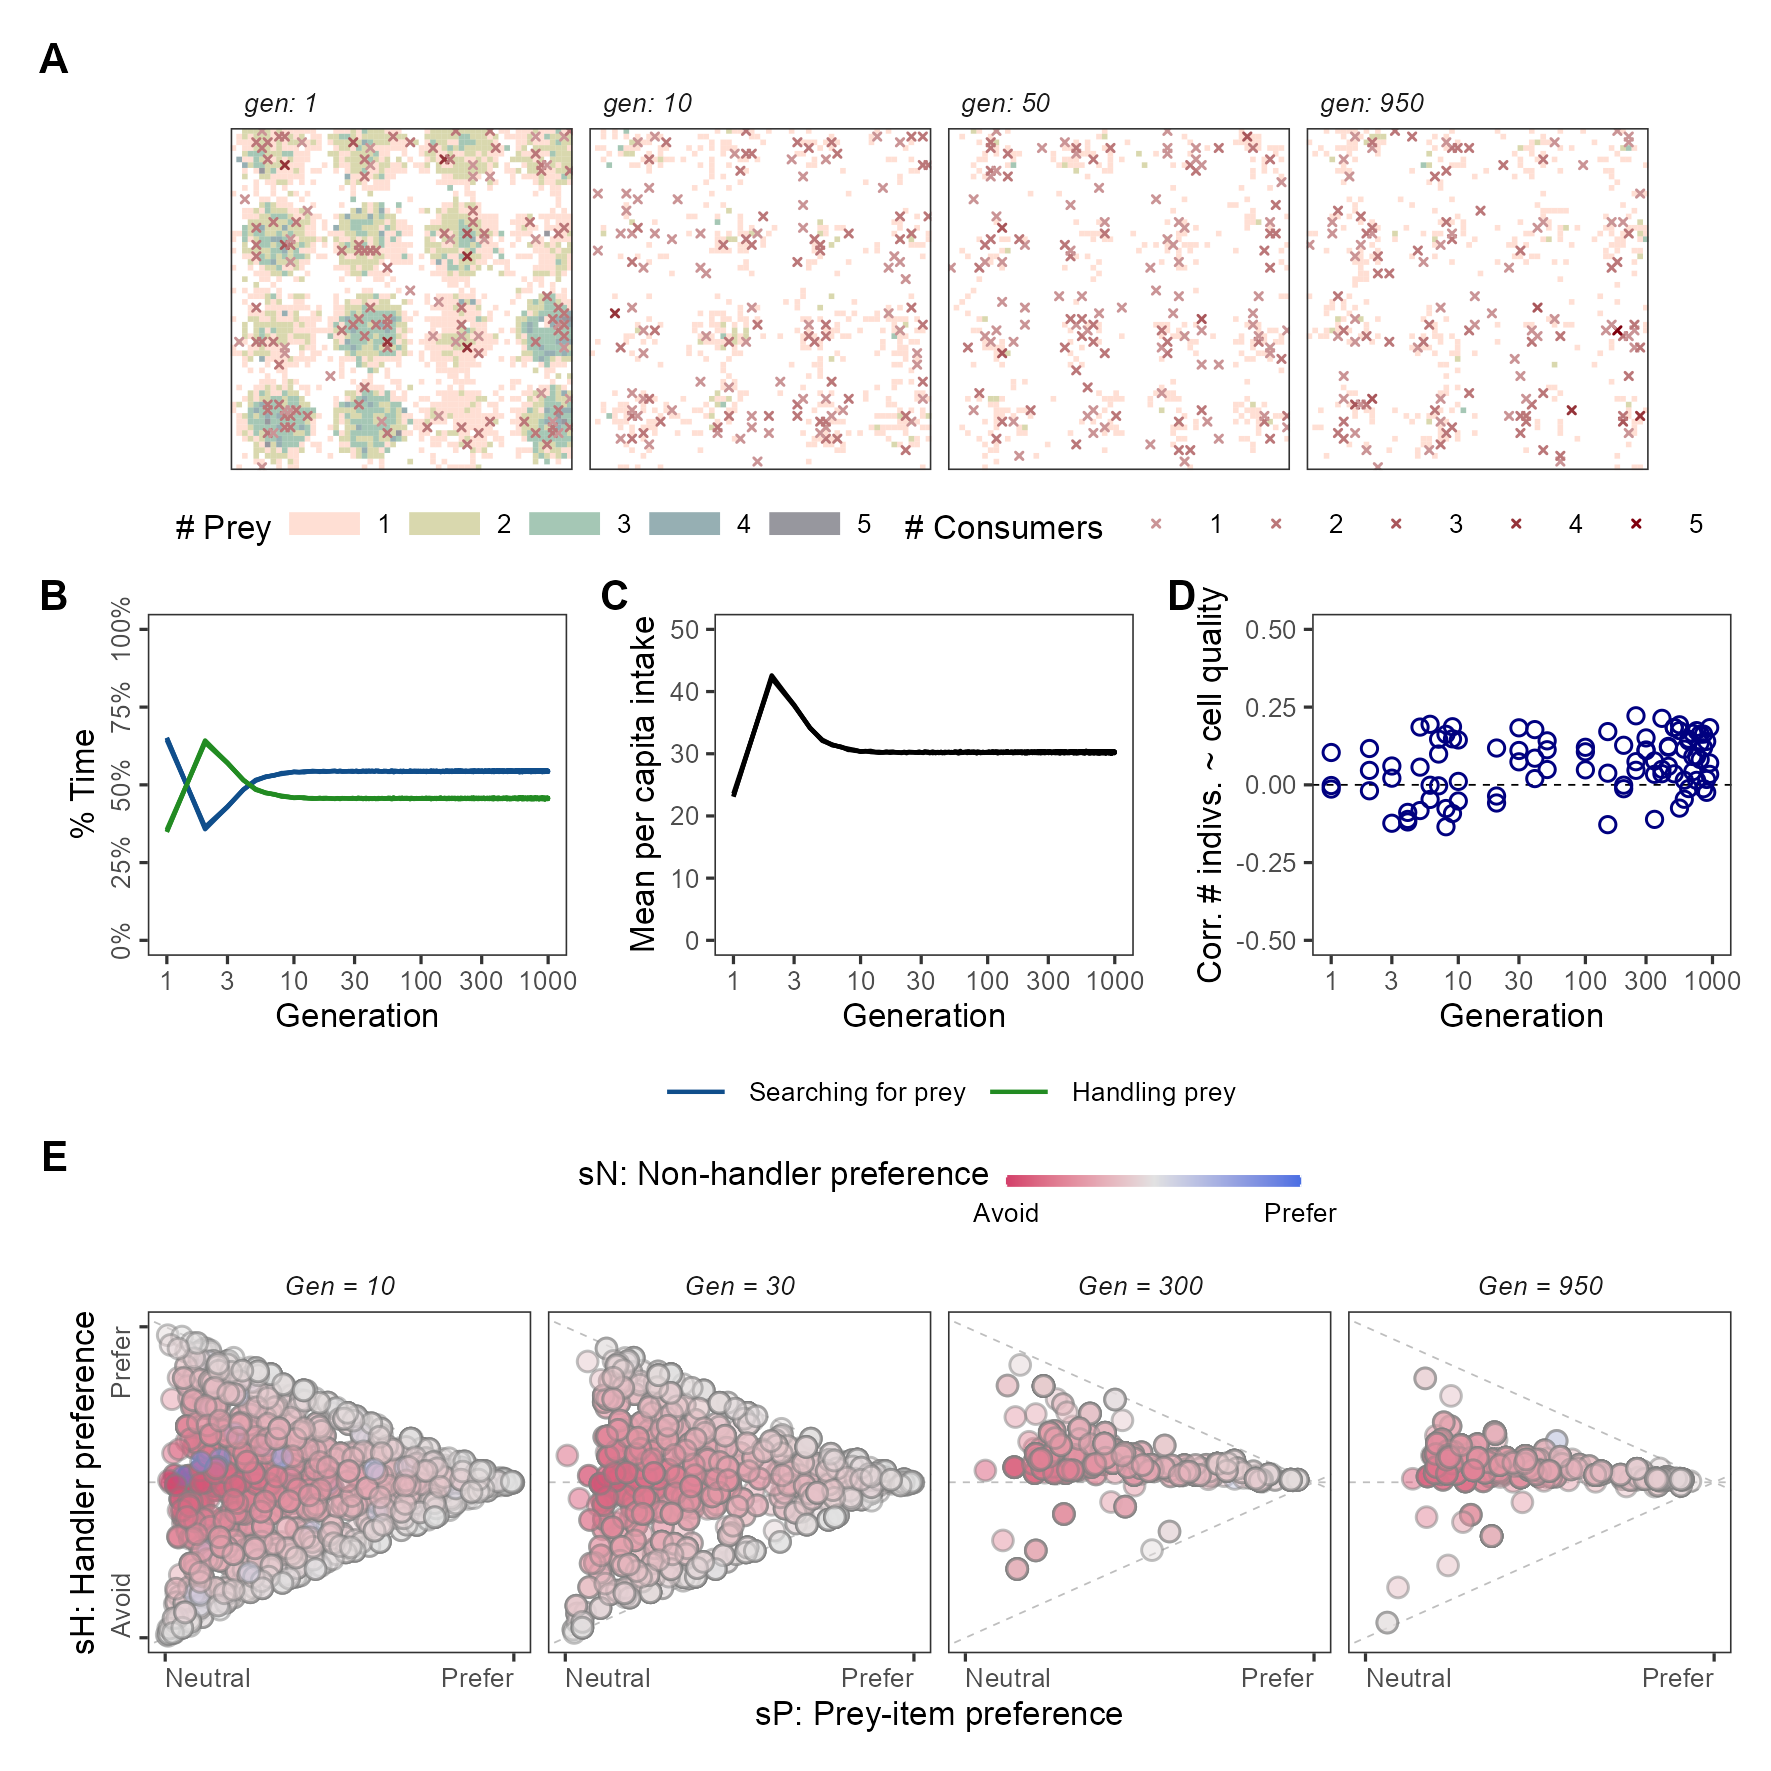
\includegraphics[width=0.7\textwidth]{figures/kleptomove/fig_01.png}
    \caption{
        \textbf{Eco-evolutionary implications of pure exploitation competition in scenario 1.}
        \textbf{(A)} A population comprised solely of foragers seeking prey on a resource landscape swiftly depletes initially abundant prey-items within 10 generations (of 1,000 simulated).
        Foragers maintain this prey-item scarcity throughout the remaining generations of the simulation, despite regular resource regeneration (see G = 950).
        \textbf{(B)} Within 20 generations of evolution, the population reaches an equilibrium in the relative proportion of time spent on searching for prey and handling prey, and in \textbf{(C)} mean per-capita intake.
        \textbf{(D)} The number of foragers per cell is only weakly correlated with cell productivity $r$, contrary to the input matching rule of Ideal Free Distribution theory.
        \textbf{(E)} A wide range of movement strategies co-exist on the landscape over hundreds of generations.
        Individuals may focus on moving up gradients of prey-items (sP $\approx$ 1.0: \textit{prefer}), moving towards successful foragers (handlers), or moving away from unsuccessful foragers which are potential competitors (sN $\approx$ red).
        Panels \textbf{A, E} show a single replicate, panels \textbf{B, C, D} and \textbf{D} show three replicate simulations with log-scaled X-axes (lines overlap almost perfectly); all panels are for $r_{max}$ = 0.01; panel \textbf{E} shows 2,500 individuals.
    }
    \label{klepto_fig_01}
\end{figure}

\subsection*{Scenario 2: Co-existence of Foragers and Kleptoparasites}

In scenario 2, with fixed foraging and kleptoparasitism allowed, the spatial distribution of prey-items at equilibrium is very different from scenario 1.
Consumers graze down resource peaks until few prey-items remain on the landscape; however, within 50 generations the resource landscape recovers with prey abundances higher than in the earliest generations (Fig.~\ref{klepto_fig_02}A).
This is because of the emergence of kleptoparasites (Fig.~\ref{klepto_fig_02}B): in early generations, kleptoparasites are rare, and the activity budget, the mean per-capita intake, and the distribution of consumers over the landscape, are similar to scenario 1.
As resources are depleted and kleptoparasite-handler encounters become more common than forager-prey encounters, kleptoparasitism becomes the majority strategy (a stable $\sim$70\% of the population; see Fig.~\ref{klepto_fig_02}B), and searching for handlers to rob becomes the commonest activity.
However, the high frequency of this activity and the low frequency of handling, indicate that few kleptoparasites are successful at robbing handlers.

With few foragers, few prey-items are extracted from the landscape, which recovers beyond its initial prey abundance within 50 generations (Fig.~\ref{klepto_fig_02}A).
As fewer prey-items are extracted overall, mean per-capita intake also declines from an initial peak (Fig.~\ref{klepto_fig_02}C).
Despite the strong spatial structure of the resource landscape within 50 generations, the correlation between consumers (of either strategy) and cell productivity remains weak or zero across generations (Fig.~\ref{klepto_fig_02}D).
This may be partially explained by the ecology of kleptoparasitism: foragers are regularly displaced by kleptoparasites, and kleptoparasites must themselves move to find handlers.

There is a sharp evolutionary divergence of movement strategies between foragers and kleptoparasites.
While both foragers and kleptoparasites evolve to prefer prey and avoid non-handlers, their response to handlers is very different (Fig.~\ref{klepto_fig_03}; see also Supplementary Material Fig.~3, 5).
Kleptoparasites very rapidly evolve a strong preference for moving towards handlers, which are their primary resource (Fig.~\ref{klepto_fig_03}).
In the absence of kleptoparasites, foragers would also evolve a similar preference (Fig.~\ref{klepto_fig_01}E), but, with kleptoparasites common in the population, foragers converge upon a handler-avoiding strategy (Fig.~\ref{klepto_fig_03}).
This completes the explanation for why consumers do not match landscape productivity: foragers evolve strategies to avoid high productivity areas (which are more likely to have many handlers), while kleptoparasites evolve strategies to find handlers (which need not be on high productivity cells).

\begin{figure}[t!]
    \centering
    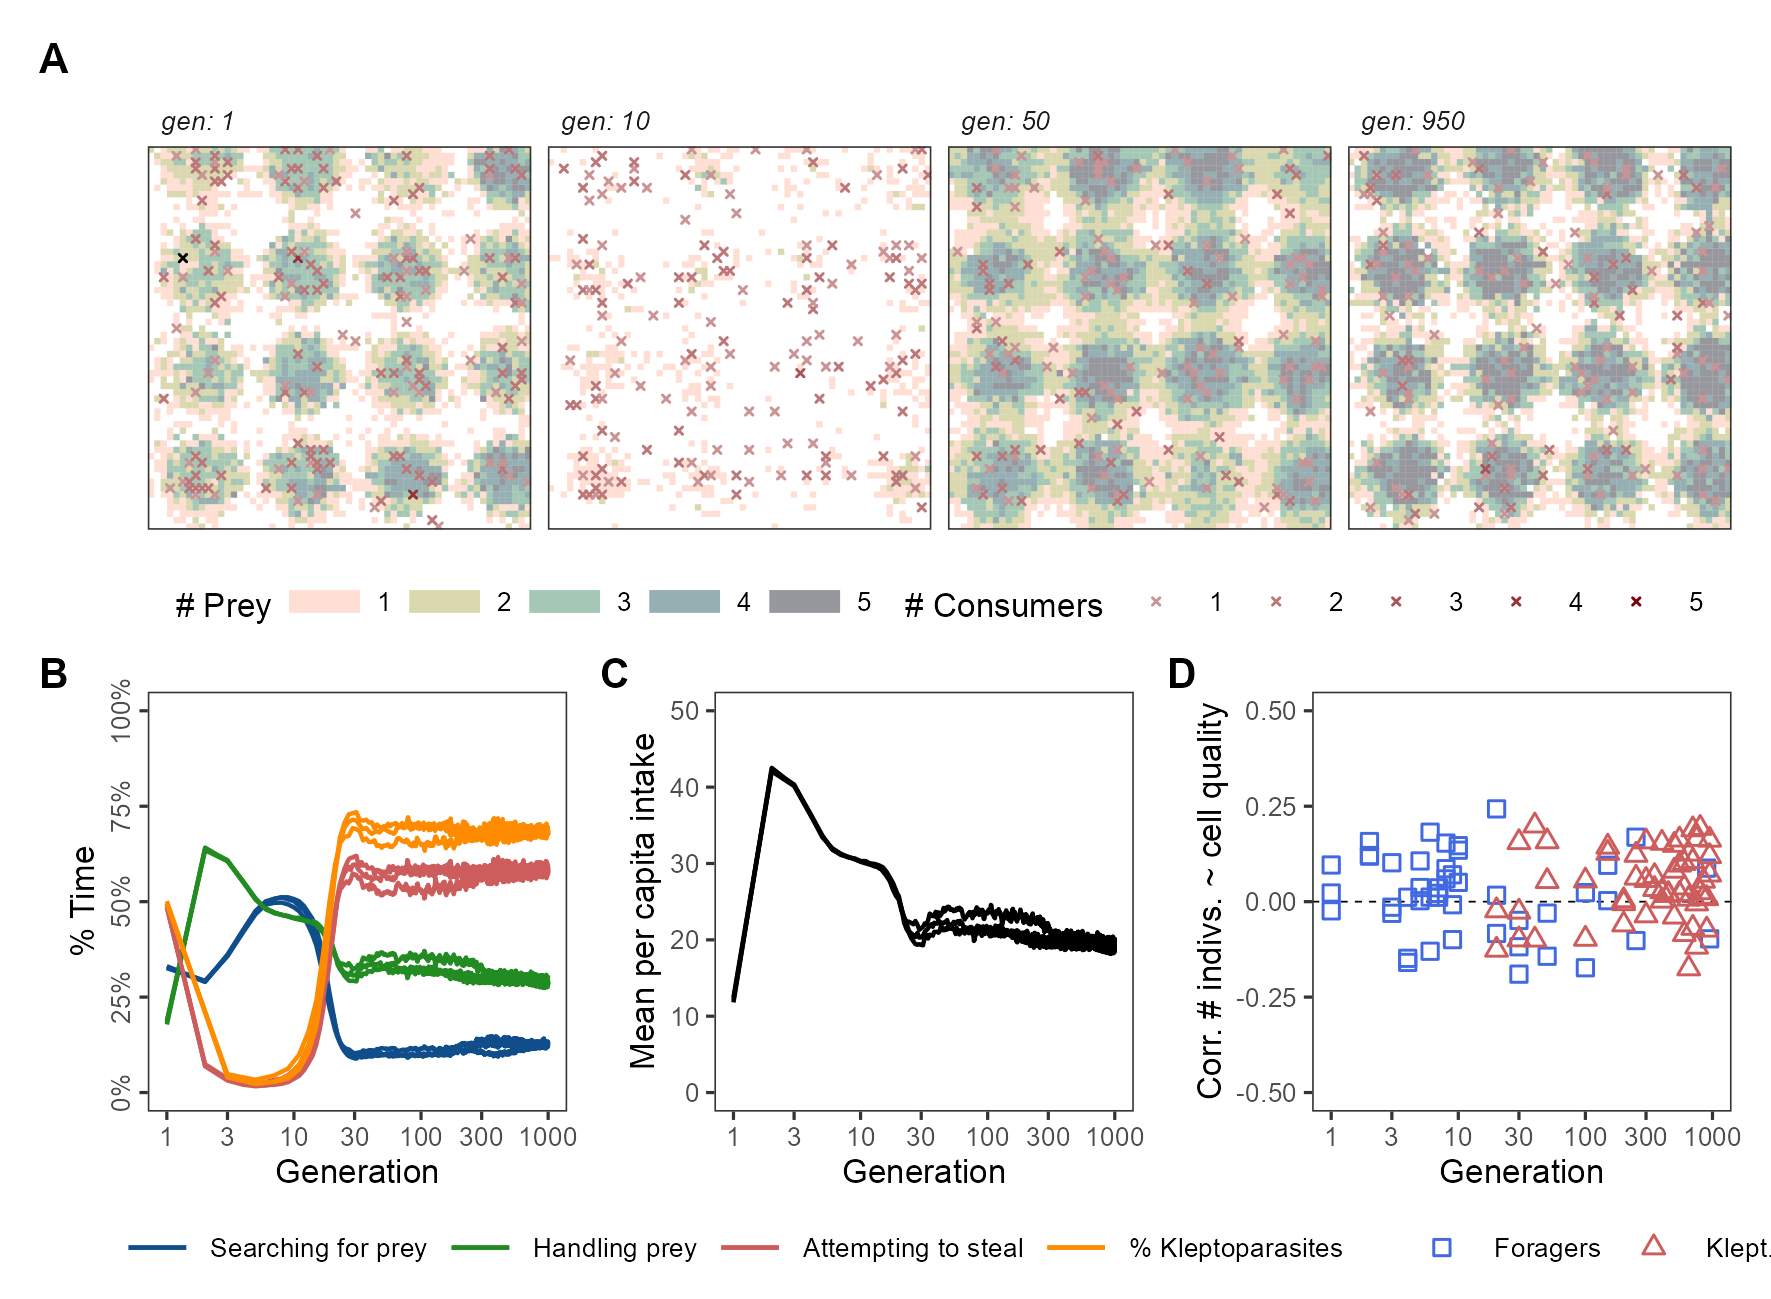
\includegraphics[width=0.9\textwidth]{figures/kleptomove/fig_02.png}
    \caption{
        \textbf{Eco-evolutionary implications of the coexistence of foragers and kleptoparasites following fixed competition strategies in scenario 2.}
        \textbf{(A)} Populations with both foragers and kleptoparasites drastically deplete the initially well-stocked resource landscape by generation 10; however, prey densities recover strongly by generation 50, even beyond the densities in generation 1.
        \textbf{(B)} A surprisingly stable equilibrium between the forager and kleptoparasite strategies is reached within 30 generations, with the relative frequency of kleptoparasites (orange line) first dropping to very low levels but later recovering to reach a high level ($\sim$ 70\%) in all three replicates.
        Consequently, at equilibrium, only about 10\% of individuals are foragers searching for prey, 50\% are kleptoparasites attempting to steal from handlers, and 40\% are handlers processing prey-items (either foragers or kleptoparasites). 
        \textbf{(C)} When kleptoparasites are rare, the population intake rate exhibits the same pattern as in scenario 1, dropping to a lower level with the emergence of kleptoparasites.
        Naturally, there is an increase in the proportion of time spent on stealing attempts (red line -- \textbf{B}), and a corresponding decrease in prey seeking (by searching foragers; blue line -- \textbf{B}), and handling (green line -- \textbf{C}).
        \textbf{(D)} Neither foragers nor kleptoparasites follow the input matching rule, and the correlation of their abundance with cell productivity $r$ is zero at equilibrium.
        Panel \textbf{A} shows a single replicate, while \textbf{B, C, D} and \textbf{D} show three replicates with log-scaled X-axes; all panels are for $r_{max}$ = 0.01.
    }
    \label{klepto_fig_02}
\end{figure}

\begin{figure}[t!]
    \centering
    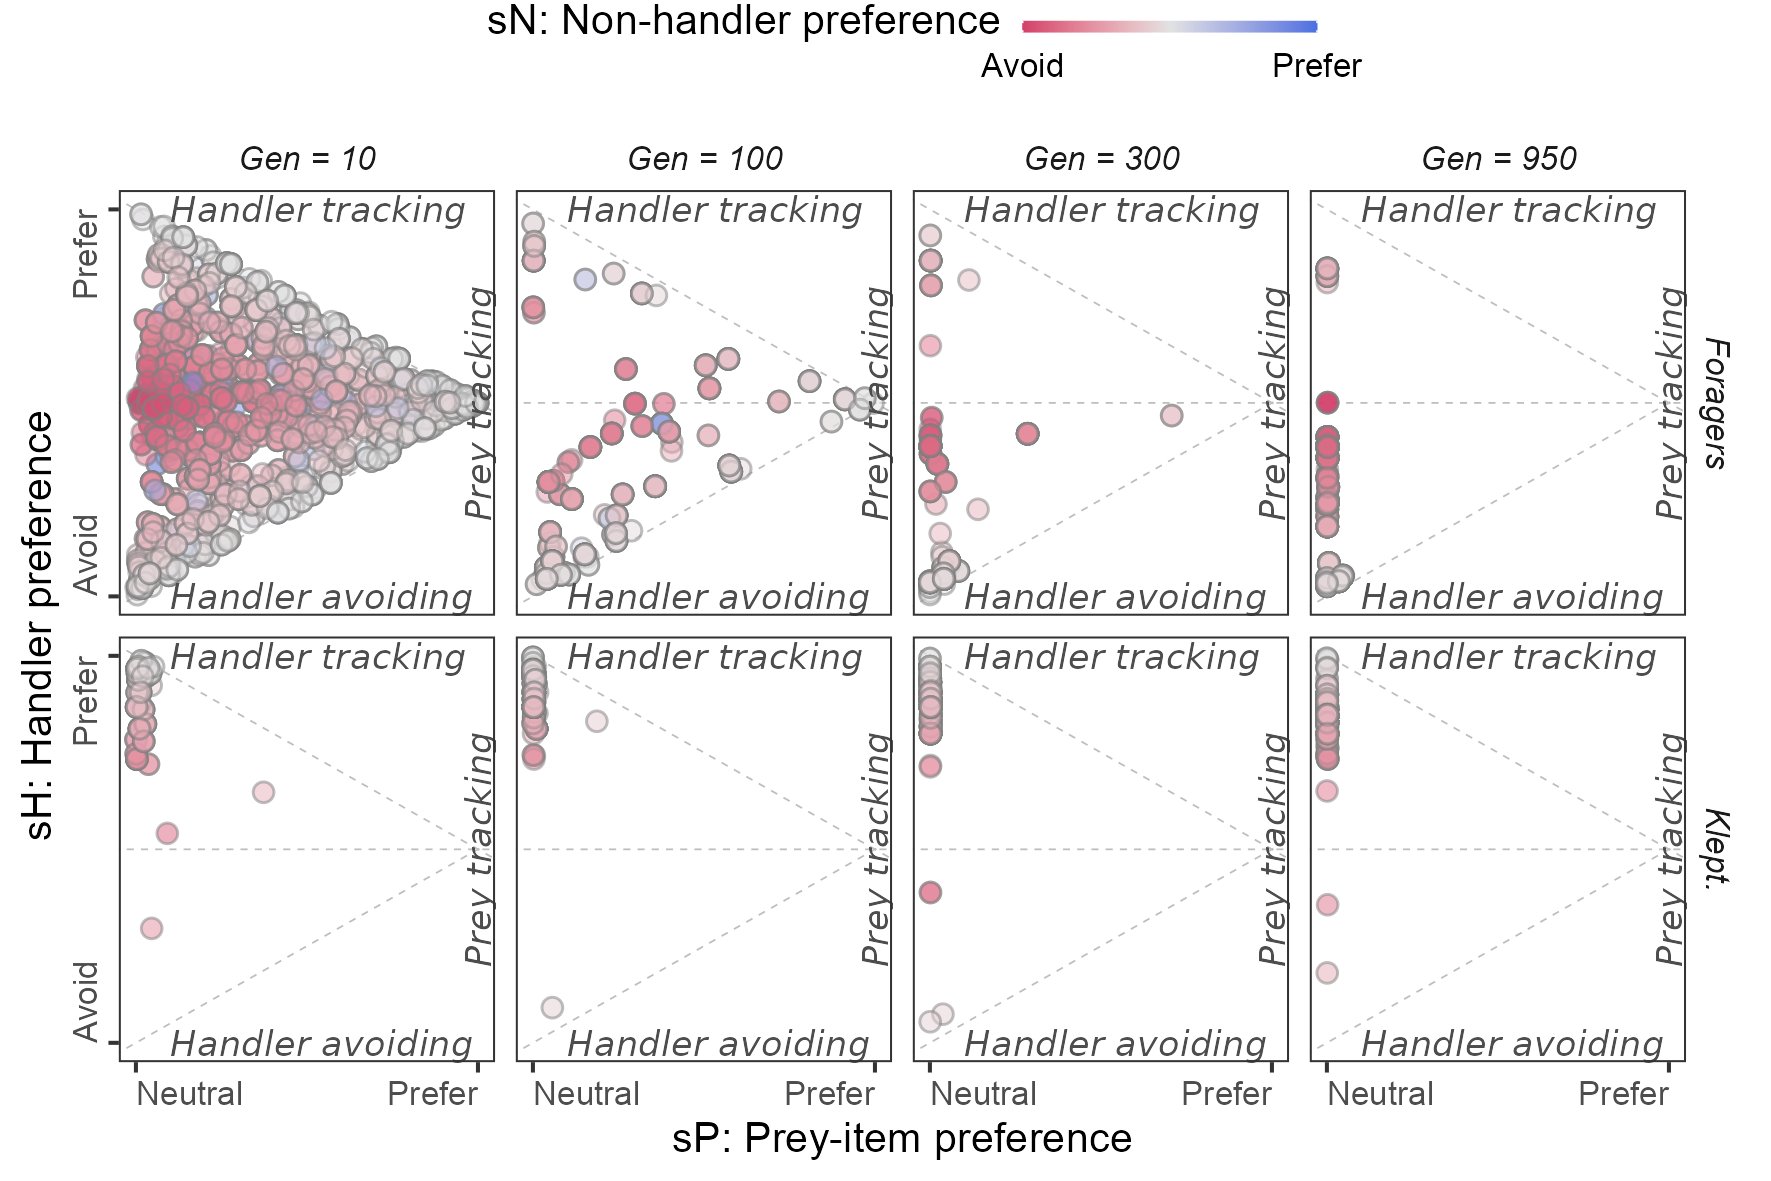
\includegraphics[width=0.9\textwidth]{figures/kleptomove/fig_03.png}
    \caption{
       \textbf{Rapid divergence of movement strategies between foragers and kleptoparasites in scenario 2.}
       In scenario 2, kleptoparasites rapidly diverge (within 10 generations) from foragers in their movement strategy, clustering around sH = 1.0: a handler-tracking strategy.
       This strategy is stably maintained throughout the simulation (G = 100, 300, 950).
       Foragers retain substantial diversity in movement strategies for many generations (see G = 100), but unlike scenario 1, tend to be repelled (relative sH < 0), as well as attracted to handlers (relative sH > 0).
       Over time, foragers adopt a strategy that helps them avoid all other individuals (G = 300, 950).
       A few individuals sporadically adopt a movement strategy associated with the opposite competition strategy; this is most likely due to mutations in the competition strategy, rather than a new movement morph within either foragers or kleptoparasites.
       At the evolutionary equilibrium then, social information (either sH or sN) is the strongest component of all individuals' movement strategies.
       All panels show 2,500 individuals (25\% of total) from the same simulation replicate ($r_{max}$ = 0.01), and earlier generations are ancestors of later generations.
    }
    \label{klepto_fig_03}
\end{figure}

\subsection*{Scenario 3: Condition-dependent Kleptoparasitism}

When individuals are allowed to choose their competition strategy (foraging or kleptoparasitism) based on local environmental cues, the distribution of prey-items is substantially different from the two previous scenarios (Fig.~\ref{klepto_fig_04}A).
Initially, individuals deplete the resource landscape of prey-items within ten generations.
By generation 50, the resource landscape recovers some of the spatial structure of early generations, but prey-item abundances do not match the recovery seen in scenario 2.
This is because unlike scenario 2, individuals search for prey more often and steal less (at or below 25\%; compare Figs.~\ref{klepto_fig_04}B and \ref{klepto_fig_02}B), preventing a full recovery of the resource landscape.
Consequently, mean per-capita intake stabilises (after an initial spike, as in scenarios 1 and 2) within ten generations to a level similar to scenario 1 (Fig.~\ref{klepto_fig_04}C).
While not as strong as predicted by IFD theory, the correlations between consumer abundance and cell productivity are weakly positive (Fig.~\ref{klepto_fig_04}D).

The weak input matching is likely because all individuals prefer to move up gradients of prey density, and towards handlers, which are more likely to be found on resource peaks (Fig.~\ref{klepto_fig_04}E; see also Supplementary Material Fig.~4, 7).
Using conditional foraging strategies, individuals are able to switch between resource types (prey and handlers) depending on which is more profitable \parencite{emlen1966} (`opportunistic kleptoparasitism'; Fig.~\ref{klepto_fig_04}F; see Supplementary Material Fig. 6).
All individuals would choose to steal when handlers are present, even when prey items are more common.
Indeed, about 40\% of individuals would choose to steal even when prey are abundant and there are no handlers at all, showing the prevalence of a `fixed kleptoparasite' clade similar to scenario 2.
In a further parallel with scenario 2, about 70\% of individuals have an intrinsic bias towards kleptoparasitism, i.e., they would by default attempt to steal when there are no cues to inform their decision (Fig.~\ref{klepto_fig_04}F: $P$ = 0, $H$ = 0).

\begin{figure}[t!]
    \centering
    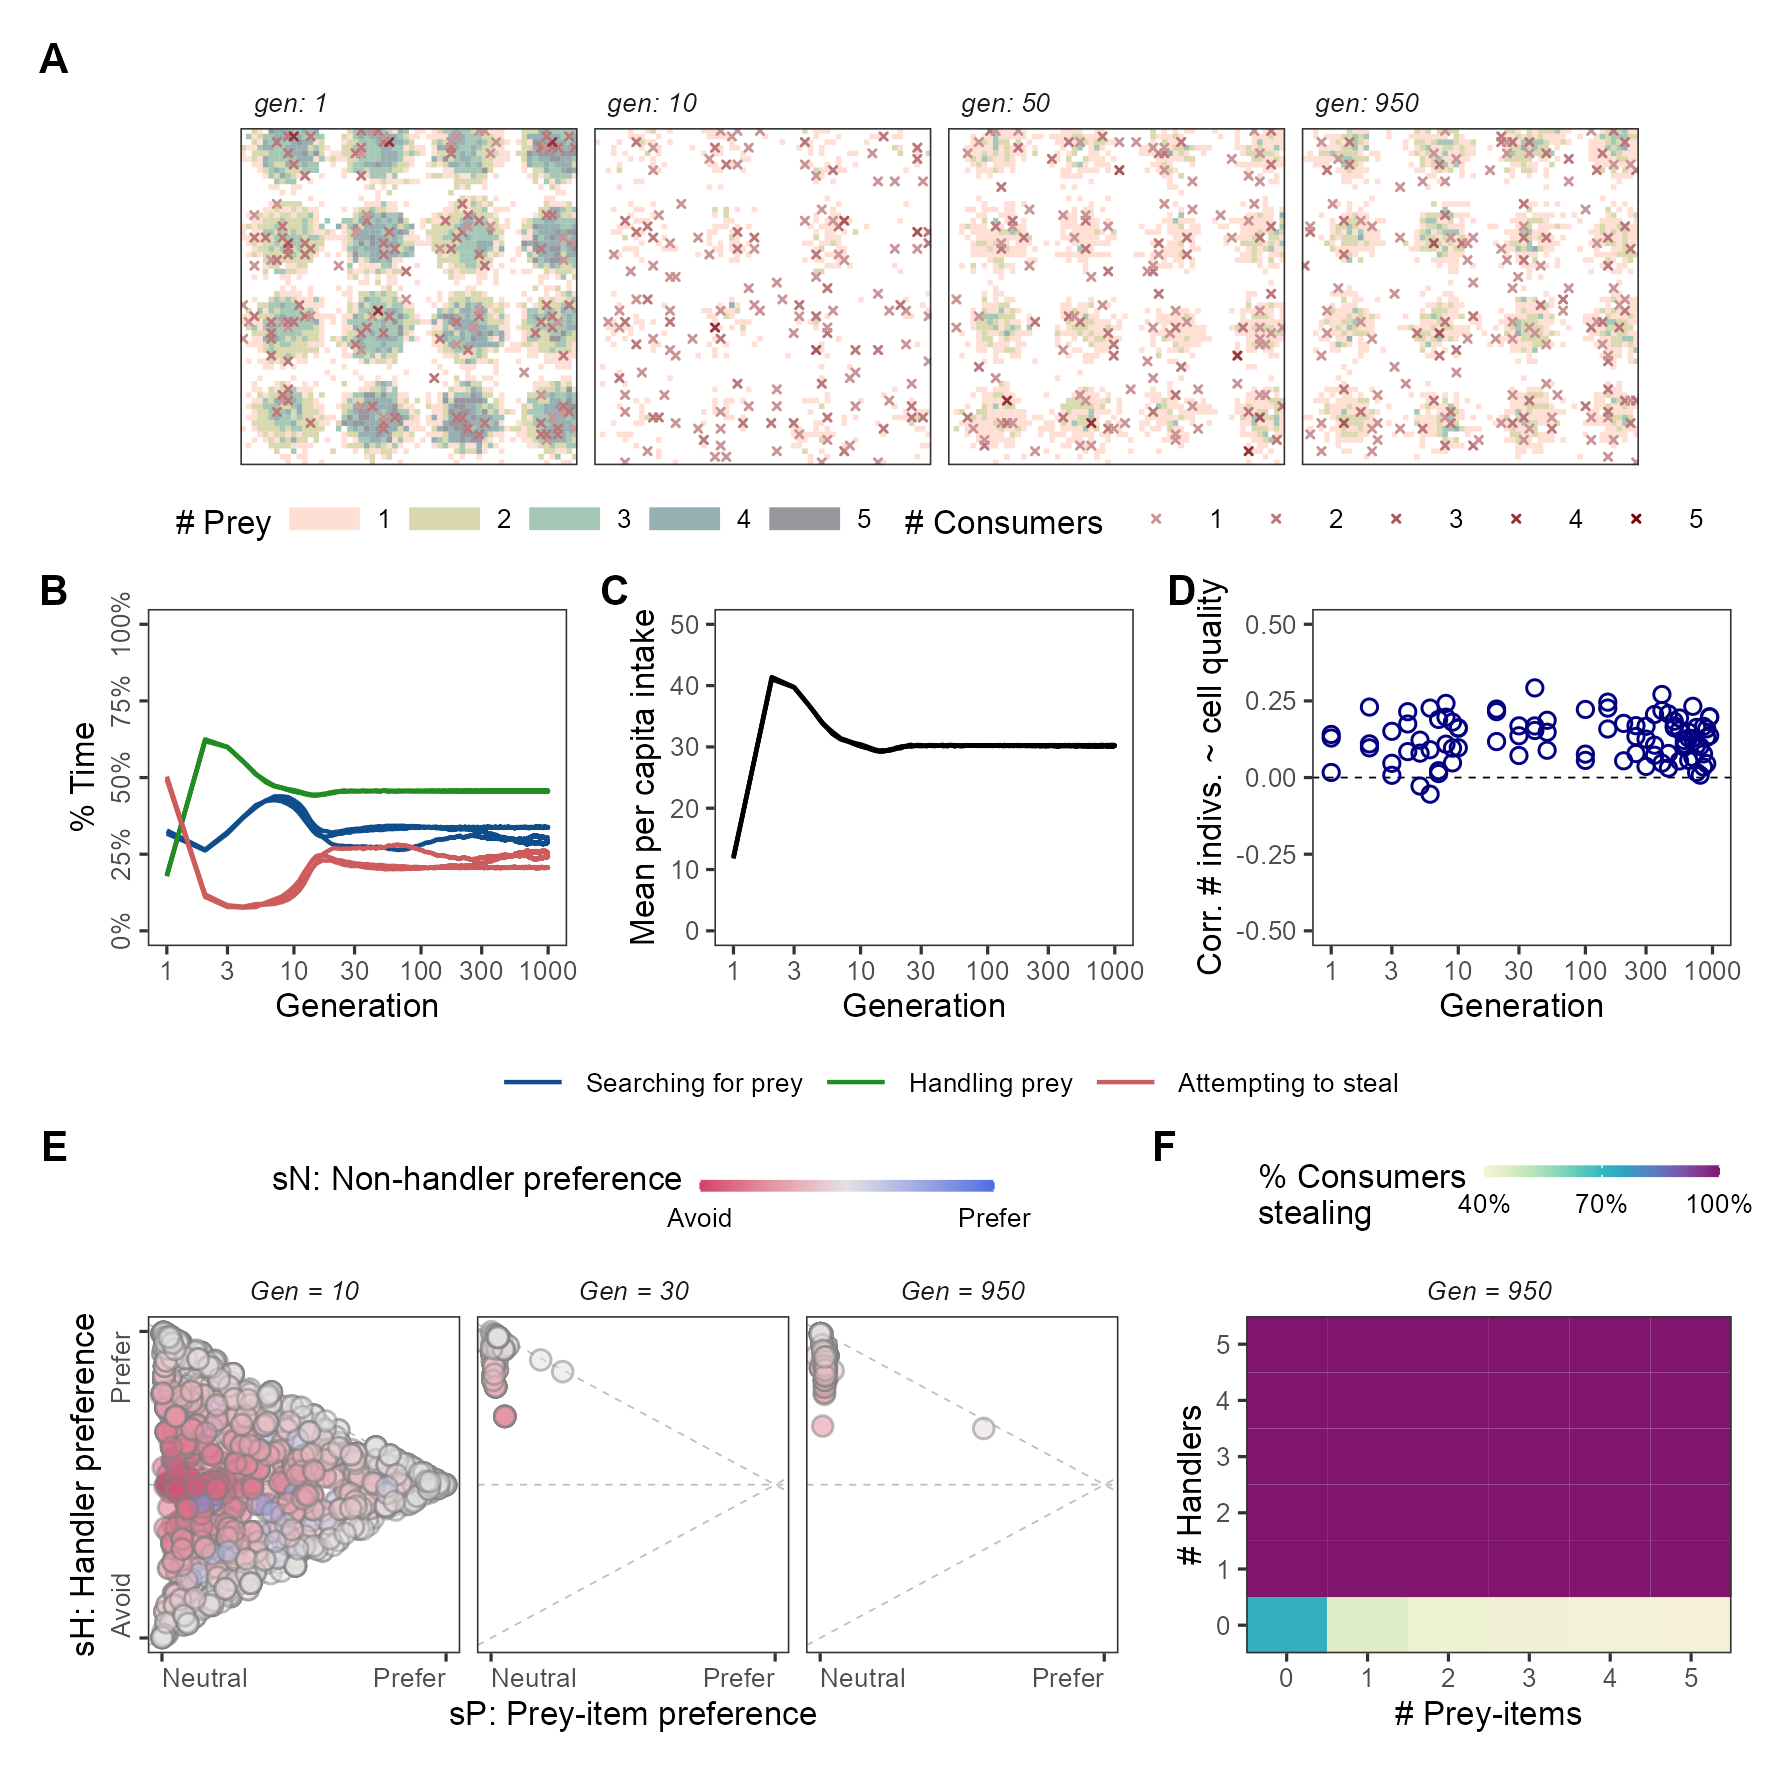
\includegraphics[width=0.9\textwidth]{figures/kleptomove/fig_04.png}
    \caption{
        \textbf{Eco-evolutionary implications of conditional foraging strategies in scenario 3.}
        \textbf{(A)} The initially well-stocked resource landscape is rapidly depleted within 10 generations, yet within 50 generations, prey abundances recover on many cells, though not to the extent of scenario 2.
        The local density of individuals on occupied cells is shown as coloured crosses. 
        \textbf{(B)} By generation 30, the proportion of time spent searching (blue line), handling (green line), and stealing prey (red line) reach an equilibrium that differs somewhat across replicates, but \textbf{(C)} the total intake of the population reaches the same equilibrium value in all three replicates.
        \textbf{(D)} The correlation between the local density of individuals on a cell, and its productivity $r$ is stronger than in scenario 2.
        \textbf{(E)} From an initially high diversity of movement strategies, there is a rapid convergence (within 30 generations) of all individuals to strongly prefer moving towards successful foragers, or handlers, nearly to the exclusion of all other movement cues.
        This handler-tracking strategy once established is maintained (Gen = 300, 950).
        \textbf{(F)} Population competition strategies are more varied. While most individuals will choose to forage as prey density increases, about 40\% of individuals attempt to steal even when prey is abundant and handlers are scarce.
        All individuals will steal when handlers are available.
        Panels \textbf{A, E} show a single replicate, while \textbf{B, C} and \textbf{D} show three replicates, \textbf{F} shows the mean across replicates; all panels are for $r_{max}$ = 0.01.
    }
    \label{klepto_fig_04}
\end{figure}

\subsection*{Movement Strategies on Depleted Landscapes}

Orienting movement towards resources \parencite[][\textit{where to move}]{nathan2008a} can be a challenge in a system with low densities of discrete prey-items, because the local prey \textit{density} may provide very limited information about local \textit{productivity}.
In our model, prey-depletion leads parts of the resource landscape to become `clueless regions' \parencite{perkins1992}, where foragers cannot make directed movements based on prey-item abundances alone, as all neighbouring item abundances are identical (see white areas in Fig.~\ref{klepto_fig_05}A; A1: scenario 1, A2: scenario 2, A3: scenario 3).
At the beginning of all three scenarios, about 75\% of landscape cells have a different number of prey-items from the cells around them; these are primarily cells with an intermediate $r$, which have more prey than peripheral cells of resource peaks, but fewer prey than the central cells.
This proportion rapidly declines to a much lower value within 10 generations in all three scenarios.

The `cluelessness' of the landscapes develops differently across scenarios on evolutionary timescales (Fig.~\ref{klepto_fig_05}B).
In scenario 1, the proportion of cells with a different number of items in the neighbourhood is initially very high (Fig.~\ref{klepto_fig_05}A1).
This proportion rapidly declines to $\sim$25\% within 10 generations, as foragers deplete most prey-items, making most of the landscape a clueless region.
In this context, foragers evolve to move towards handlers, with $>$ 75\% of individuals showing a preference for handlers within 100 generations (Fig.~\ref{klepto_fig_05}B1).
Forager preference for handlers may be explained as the sensing of a long-term cue of local productivity.
Since handlers are immobilised on the cell where they find a prey-item, handler density is an indirect indicator of cell $r$, and due to spatial autocorrelation, also of the $r$ of bordering cells.

Scenario 2 landscapes develop similarly to scenario 1 in early generations (Fig.~\ref{klepto_fig_05}A2).
However, within 50 generations, most cells bear items as extraction is reduced, with differences among cells according to their $r$ (see also Fig.~\ref{klepto_fig_02}A).
Thus $>$ 75\% of cells have a different number of items from neighbouring cells (Fig.~\ref{klepto_fig_05}A2 -- panel \textit{gen: 50}, 5B2).
Unlike scenario 1, the rapid increase in handler preference is driven by kleptoparasites becoming the majority strategy (see above).
Scenario 3 is similar to scenario 2, except that only about half of all cells have a different number of prey-items from neighbouring cells (Fig.~\ref{klepto_fig_05}A3, 5B3).
Here, the rapid evolution of a handler preference in movement decisions cannot be assigned a clear cause, since handlers are both a potential direct resource as well as indirect cues to the location of productive cells.

\begin{figure}[t!]
    \centering
    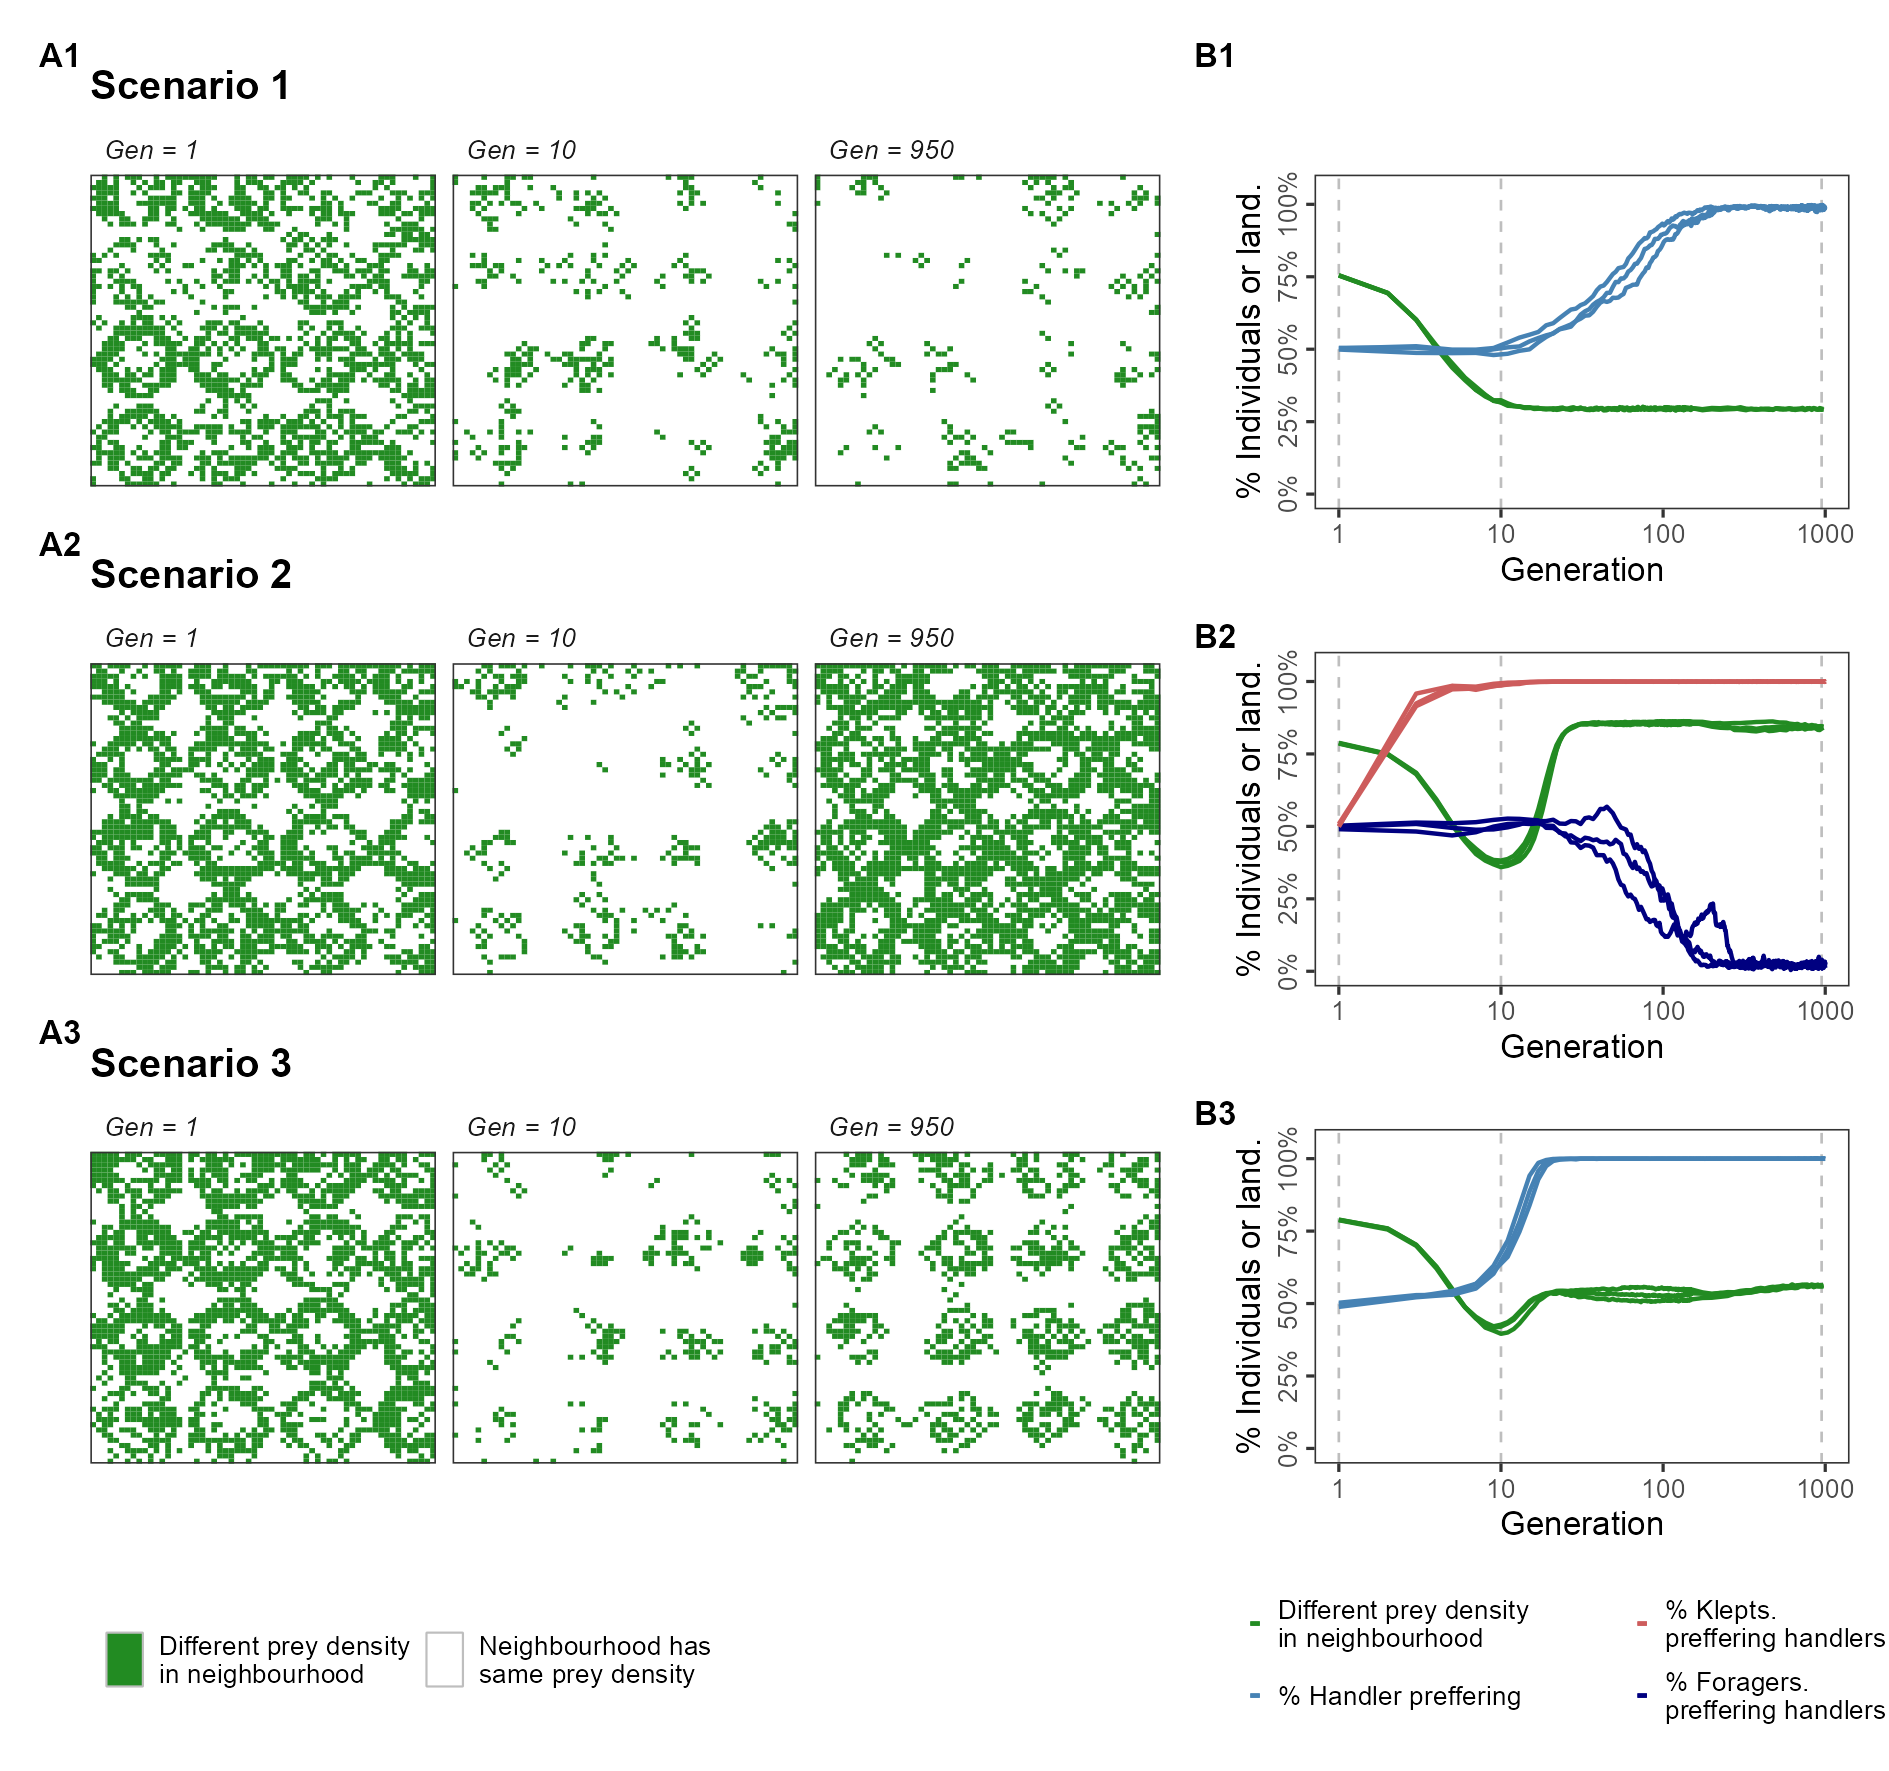
\includegraphics[width=0.9\textwidth]{figures/kleptomove/fig_05.png}
    \caption{
        \textbf{Uninformative prey densities and the evolution of social information as an alternative movement cue.}
        \textbf{(A1, A2, A3)} On cells coloured green, local prey densities are informative for movement, as the central and neighbouring cells have different prey densities.
        While differences in local prey densities provide informative cues for `adaptive' movement in early generations, this is much less true once the resource landscape is depleted of prey-items (depending on the scenario).
        \textbf{(B1, B2, B3)} The proportion of cells where differences in local prey densities provide informative movement cues (green line), and the proportion of individuals preferring to move towards handlers (blue line), whose presence may be used as an alternative cue for movement towards higher-productivity areas of the landscape.
        In \textbf{(B2)} representing scenario 2, this proportion is shown separately for foragers (blue line) and kleptoparasites (red line).
        While panels in \textbf{(A)} show a single representative replicate for $r_{max}$ = 0.01, panels in \textbf{(B)} show three replicates.
    }
    \label{klepto_fig_05}
\end{figure}

\subsection*{Effect of Landscape Productivity}

The prey-item regrowth rate that characterises the peaks of the resource landscape ($r_{max}$) is a measure of the productivity of the resource landscape overall. 
Having thus far focused on scenarios with $r_{max}$ = 0.01 (corresponding to a peak production of 4 food times per consumer lifetime), we find that, not unexpectedly, the value of $r_{max}$ has a marked effect on evolved population activity budgets, mean per capita intake, and even evolved strategies.
The frequency of foraging reduces with $r_{max}$ in scenarios 1 and 3; this is caused by more frequent acquisition of prey-items (as regrowth keeps pace with depletion), which results in a greater frequency of handling rather than foraging.

In scenario 2 however, the frequency of handling is relatively unaffected by increasing $r_{max}$ (Fig.~\ref{klepto_fig_06}A).
The difference between scenarios 2 and 3 has to do with the change in the frequency of kleptoparasitism (Fig.~\ref{klepto_fig_06}B).
In scenario 2, kleptoparasitism forms $>$ 75\% of all activities at low $r_{max}$, and is much more common than in scenario 3 populations at the same regrowth rate.
However, at relatively high $r_{max}$ (0.03), the fixed kleptoparasitic strategy goes extinct.
This is because at high $r_{max}$, forager-prey encounters are more common than kleptoparasite-handler encounters, in both early ($<$ 10) and later generations ($>$ 50).
Consequently, kleptoparasites have relatively much lower fitness than foragers, and do not proliferate.
Thus at high $r_{max}$, a scenario 2 population is nearly identical to a scenario 1 population; while some kleptoparasites may be seen in later generations, these occur most likely due to ephemeral mutations in the forager strategy.

In scenario 3, kleptoparasitism persists at low frequencies even at the highest regrowth rates (Fig.~\ref{klepto_fig_06}B); thus some foragers lose time in extracting items which are then stolen from them.
Consequently, while populations in all three scenarios achieve very similar mean per-capita intakes at low $r_{max}$, at intermediate regrowth rates (0.01, 0.02), conditionally kleptoparasitic populations achieve a higher mean per-capita intake than populations using fixed strategies.
Only at high $r_{max}$, when fixed strategy populations effectively convert to purely forager populations, do they achieve a higher intake than conditional strategy populations (Fig.~\ref{klepto_fig_06}C).

\begin{figure}[t!]
    \centering
    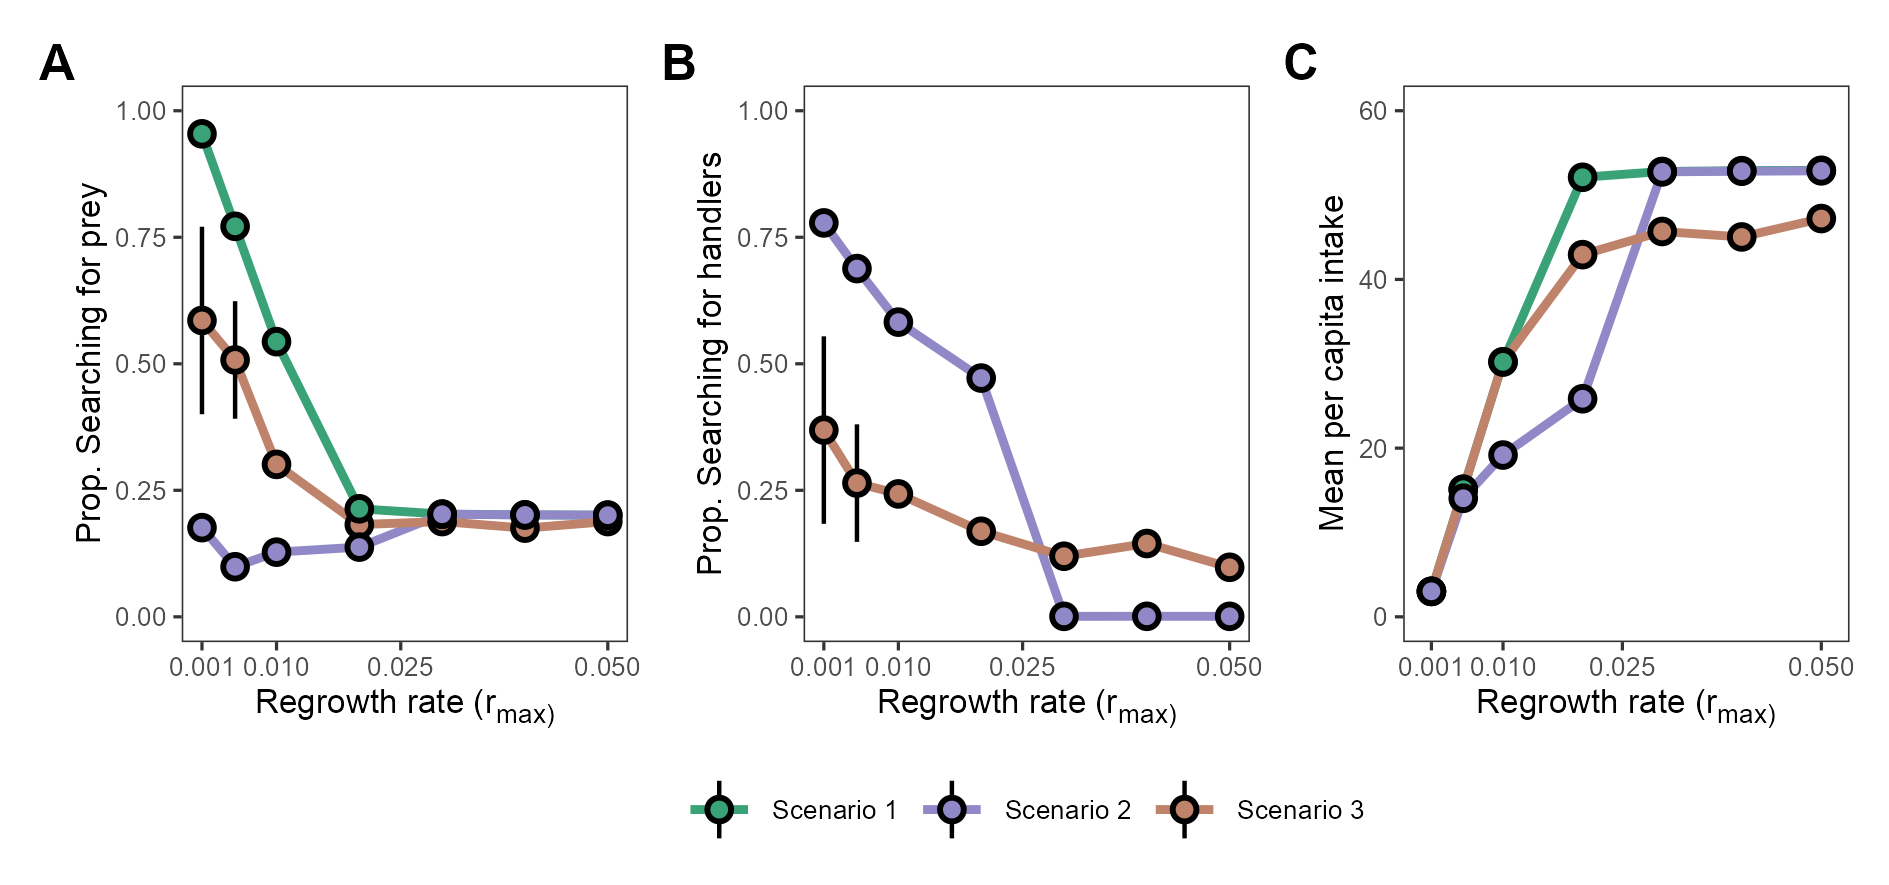
\includegraphics[width=\textwidth]{figures/kleptomove/fig_06.png}
    \caption{
        \textbf{Landscape productivity strongly affects scenario outcomes.}
        \textbf{(A)} The proportion of time spent searching for food decreases with increasing $r_{max}$ in scenarios 1 and 3 but remains relatively stable within scenarios. 
        This is partly due to a higher proportion of time spent handling at higher prey densities. 
        \textbf{(B)} The proportion of time spent searching for handlers (in order to steal prey from them) also decreases with increasing $r_{max}$. 
        In scenario 2, kleptoparasites go extinct for $r_{max}$ values above 0.025. 
        \textbf{(C)} At low productivity, the average intake is similar in all three scenarios. 
        For higher $r_{max}$ values the average intake rate is lowest in scenario 2, until $r_{max}$ is larger than 0.025 and kleptoparasites go extinct (leading to the same kind of population as in scenario 1). 
        At high $r_{max}$, the average intake rate in populations with conditional kleptoparasites (scenario 3) is substantially lower than in populations without kleptoparasitism.
        All panels show conditions at G = 1,000; error ranges where present show standard deviation around values; some error ranges are too small to be visible.
    }
    \label{klepto_fig_06}
\end{figure}

\section*{Contextualising the Outcomes of the Kleptomove Model}

Our spatially-explicit individual-based model implements the ecology and evolution of movement and foraging decisions, as well as resource dynamics, in biologically plausible ways, and offers a new perspective on the distribution of animals in relation to their resources under different scenarios of competition.
%%
First, individuals moving with a limited perception range and competing only by exploitation, evolve movement strategies for both direct and indirect resource cues (prey-items and handlers, respectively).
Regardless, on a resource landscape with discrete prey-items, large areas may become devoid of any movement cues, leading to a mismatch between individual distribution, prey-item distribution, and landscape productivity.
%%
Second, interference competition in the form of kleptoparasitism rapidly establishes itself on landscapes where stealing is more time-efficient than searching for prey, even when such interference is a fixed strategy and kleptoparasites cannot forage for prey.
This rapid increase in kleptoparasitism as a strategy is accompanied by the divergent evolution of movement strategies that favour moving towards handlers, which are the primary resource of the kleptoparasites.
In this sense, obligate kleptoparasites may be thought of as forming a higher trophic level, with handlers as their prey.
%%
Third, when foraging strategy is allowed to be conditional on local cues, \textit{(1)} the population's mean per capita intake is significantly higher than that of a population with fixed strategies, and \textit{(2)} unlike fixed strategy populations, kleptoparasitism as a strategy does not go extinct on high-productivity landscapes.
%%
However, across scenarios, individuals are broadly unable to match the productivity of the resource landscape, contrary to the predictions of IFD based models, which predict input matching for some \parencite{parker1986,holmgren1995,hamilton2002}, or all of the competitive types \parencite{korona1989}.

\subsection*{Comparison with Existing Models}

Existing models of competition and movement impose fixed movement rules on individuals to mimic either ideal or non-ideal individuals \parencite{vickery1991,cressman2006,amano2006b,beauchamp2008,stillman2010,white2018}.
When individual competitive strategies are included in models, they represent differences in competitive ability \parencite[e.g.][]{parker1986,holmgren1995,hamilton2002}, or a probabilistic switch between producing and scrounging \parencite{beauchamp2008}.
In contrast, our model allows individuals' movement (and competition) decisions to be adaptive responses to local environmental cues.
Similar to \textcite{getz2015,getz2016} and \textcite{white2018}, our individuals choose from among the available movement options after weighing the local environmental cues, similar to step selection functions \parencite{fortin2005, avgar2016, white2018}.
Local environmental cues are constantly changing, as we model discrete, depletable prey-items, contrasting with many IFD models \parencite[][]{tregenza1995,amano2006b}.
This allows for a more plausible, fine-scale consideration of exploitation competition, which is often neglected, and allows the cues sensed by individuals to strongly structure the distribution of competitors (see below).

Adaptive responses must have an explicit evolutionary context, and consider multiple generations of the population.
We follow \textcite{beauchamp2008} and \textcite{getz2015} in allowing the cue preferences that decide movement, and variation therein, to be the outcomes of natural selection.
However, instead of using `evolutionary algorithms' \parencite{beauchamp2008,getz2015,getz2016} to `optimise' individual movement rules, we consider a more plausible evolutionary process: \textit{(1)} Instead of allowing the fittest 50\% of the population to replicate, the number of offspring are proportional to individual fitness.
\textit{(2)} The cue preferences are subject to mutations independently, rather than subjecting all preferences of an individual to simultaneous mutation.
\textit{(3)} Finally, we avoided `simulated annealing', which adapts the mutation rate or the mutational step sizes to the rate of evolutionary change.
Instead we drew mutation sizes from a Cauchy distribution, so that most mutations are very small, but large-effect mutations do rarely occur throughout the simulation.
Similarly, rather than determining competition strategy probabilistically or ideally \parencite{vickery1991,beauchamp2008,tania2012}, our individuals' competition decisions are also shaped by selection (in scenarios 2 and 3).

\subsection*{Evolution of Movement Strategies Using Social Information}

In scenario 1, depletion of discrete prey can leave many areas empty of prey-items: in such areas, movement informed by a resource gradient is impossible, and individuals may move randomly \parencite[][]{perkins1992}.
This lack of direct resource cues for locally optimal movement might be among the mechanisms by which unsuitable `matrix' habitats modify animal movement on heterogeneous landscapes \parencite{kuefler2010}.
When individuals do not sense resource gradients, the presence of more successful conspecifics may indicate a suitable foraging spot \parencite[local enhancement;][]{giraldeau1999,beauchamp2008,cortes-avizanda2014}.
The presence of unsuccessful individuals, meanwhile, may signal potential costs from exploitation or interference competition.
This selects for movement strategies incorporating the presence and condition of competitors into individual movement decisions, or \textit{social movement strategies} \parencite[see e.g.][]{guttal2010}.
Consequently, consumer aggregation --- often explained by invoking external costs such as predation \parencite{krause2002,folmer2012} --- could also be the outcome of movement strategies that have evolved to trade competition costs for valuable social information on the underlying spatial structure (here, $r$) of uninformative landscapes \parencite[][]{folmer2010,cortes-avizanda2014}.

\subsection*{Individual Variation in Movement Strategies}

Our movement strategies, comprising preferences for local ecological cues, may lead individuals to move in ways that are potentially unique to each individual.
These strategies may not maximise their intake over short timescales (a few timesteps), but their coexistance implies equivalent fitness overall.
This makes them consistent with prevalent ideas about consistent individual differences in behaviour, or `animal personalities' \parencite{wolf2012,laskowski2013,spiegel2017,shaw2020}.
In scenario 1, the persistence of multiple movement strategies across generations indicates that they have equivalent fitness \parencite[see][]{getz2015}, and that there are multiple ways to navigate a heterogeneous environment \parencite{wolf2010,shaw2020}.
Such differences may help reduce competition as individuals make subtly different movement decisions when presented with the same cues \parencite[][]{wolf2012,laskowski2013}.
Interestingly, scenario 3 has the least individual variation in movement rules, presumably because plasticity in competition strategy reduces the need for such diversification \parencite{pfennig2010}.

Scenario 2 cautions that \textit{(1)} Individual variation may only be evident when accounting for the main driver of movement decisions ($s_H$ or $s_N$; {see Supplementary Material Fig. 8 for scenario 3 as well).
\textit{(2)} Spatial context determines whether individual differences in movement strategy lead to functional variation in movement outcomes.
Subtle variation in relative prey density preferences ($s_P$) could be revealed if individuals were measured in isolation, and could lead to differences in movement paths (given a continuous gradient in prey cues).
However, in natural settings with substantial collective behaviour, different social movement strategies (correlated with foraging competition strategy) would be the primary driver of movement.
Overall, then, \textit{(a)} measuring movement behaviour in settings that correspond to animals' evolutionary context, and \textit{(b)} accounting for movement-competition strategy correlations, are both key when studying how individual differences translate to functional consequences.

\subsection*{Competition Strategies and the Ideal Free Distribution}

IFD models predict that individual movement should result in consumer distributions tracking the profitability of resource patches \parencite{fretwell1970,parker1978}, with dominant competitive types (including kleptoparasites) monopolising the best patches \parencite[][]{parker1986,holmgren1995,hamilton2002}, though \textcite{korona1989} predicts otherwise.
In scenarios 2 and 3, kleptoparasitic individuals unsurprisingly and rapidly evolve to track handlers (a direct resource), while avoiding non-handlers (potential competitors).
However, these evolved rules do not lead kleptoparasites to occupy the best cells as predicted by \citealp{parker1986}, \citealp{holmgren1995}, and \citealp{hamilton2002}.
Across our scenarios (including scenario 1), local population density is only weakly correlated with cell productivity, and is not stronger than if individuals were moving randomly (see Supplementary Material Fig. 1).
In scenario 2, this departure from predictions is driven by the contrasting movement rules of foragers, which evolve to \textit{avoid} handlers as well as non-handlers, both of which might be kleptoparasites \parencite[cryptic interference; seen in interference-sensitive shorebirds][]{bijleveld2012a}.
Thus, foragers likely avoid resource peaks, which are more likely to have handlers \parencite[due to the higher probability of forager-prey encounters][]{parker1986,holmgren1995,hamilton2002}.
Fixed kleptoparasites cannot extract prey themselves, and must move off resource peaks to track and rob handlers \parencite[similar to][]{parker1986}, breaking the link between individual density and productivity.
This shows the pitfalls of simplistically linking current ecological conditions with population distributions without considering competitive strategies or evolutionary history.

\subsection*{Constraints on Competition Strategies}

Foraging strategies involving specialisation on a resource type are expected to be constrained by the availability of that resource. 
Thus kleptoparasitism, seen as a prey-choice problem, should be constrained by the density of targets \parencite{ens1990}.
In scenarios 2 and 3, more kleptoparasitism should be expected with increasing $r_{max}$, as prey and consequently, handlers, are expected to be more abundant.
Instead, kleptoparasitism declines with increasing $r_{max}$, in line with \textcite{emlen1966}, who predicted that the commoner food type (prey) rather than the more efficiently exploited one (handlers) should be preferred.
This prey choice problem, playing out at evolutionary scales, leads kleptoparasites in scenario 2 to go extinct when prey are very common at high $r_{max}$.
At stable population densities, the persistence of fixed kleptoparasitism depends on their intake \textit{relative to foragers}.
Modelling discrete prey-items and individuals in a spatial context, then, leads to the finding that obligate kleptoparasitism is only a viable strategy when forager-prey encounters are less common than kleptoparasite-handler encounters.
Reducing the relative profitability of kleptoparasitism in other ways --- such as imposing a cost on kleptoparasitic attacks for the initiator, or reducing the probability of success (currently, 1.0) --- would also lead to a reduced incidence of kleptoparasitism, and eventual extinction even on less productive landscapes.
In scenario 3, about 40\% of individuals choose to attempt to steal even when prey are available and handlers are not.
This suggests a more realistic proportion of consistently kleptoparasitic individuals among populations with flexible foraging strategies.
Many seabirds, which forage for prey when they are super-abundant, but also readily harass other birds for prey, are a good example \parencite{brockmann1979}.
Finally, comparing across regrowth rates shows why possibly cryptic behavioral complexity should be considered in predictions of the long-term effect of environmental change on populations.
While both scenario 1 and 2 populations appear identical at high $r_{max}$, even a small decrease in environmental productivity could lead to an abrupt drop in per-capita intake --- and potentially, strongly reduced growth or survival --- for fixed strategy populations due to unexpected, emergent kleptoparasitism.

% \subsection*{Comparison with Conceptual Models}

% Classical models of animal movement and foraging largely consider homogeneous populations and environmental conditions, and movements that are made either optimally or at random.
% While these models provide powerful insights, 
% % they also have important drawbacks: individual variation, local environmental conditions, and the mechanisms of movement and decision-making cannot be adequately addressed. 
% % This is the strength of 
% individual-based models such as ours have the advantage that they can accommodate individual variation, local environmental conditions, and the mechanisms of movement and decision-making.
% % : the individual-level perspective can accommodate local circumstances, mechanisms and state variables in considerable depth and detail. 
% Individual-based modeling has the obvious drawback that numerous specific assumptions have to be made, which might not all be founded on empirical evidence, and might seem to limit the generality of the conclusions. 
% Nevertheless, as long as these models are not mistaken for attempts at faithful representations of real systems, their exploration provides valuable perspectives on the conceptual models that have dominated theory in the past. 
% After all, traditional models also include numerous assumptions (the spatio-temporal structure, the timing of events, the distribution and inheritance of traits) that are usually not stated and therefore less visible.
% For the future, we envisage pluralistic approaches, where both types of model are applied to the same research question. 
% Only comparing the outcomes of diverse models will reveal which conclusions and insights are robust, and which reflect peculiarities of the model structure.
% Only such model comparison can tell us whether and when simple models produce general insights, where simple models fail, and when mechanisms can explain initially counterintuitive observations, such as the attraction to competitors that we observed in our study.

\subsection*{Individual-Based Models in Animal Movement Ecology}

Linking individual-based models with empirical data is difficult, and is still rarely used \parencite[see works tailored to management:][]{stillman2010,diaz2021}.
Animal tracking technology is only on the cusp of allowing us to track entire populations (though small ones), and classifying their behaviour at the fine temporal scales of animal decision-making \cite[Nathan et al. in press. \textit{Science}; see e.g.][]{lieber2021, sankey2021}.
Classifying dyadic and collective behaviour from animal tracking is especially challenging \parencite{sankey2021,vissat2021}; this makes the detection of rapid competitive interactions in large populations unlikely.
Instead, experimental approaches may reveal movement strategies that reduce competitive interactions \parencite{vahl2005,vahl2005a,rutten2010, bijleveld2012a}.
However, consistent behaviour in cue-poor captive environments does not always translate to consistency in natural settings with abundant resource cues \parencite{carter2013}.

Animal movement ecology takes an explicitly individual-based approach, centred around individual decisions \parencite{nathan2008a}.
This makes individual-based models a good choice when seeking general insights into the evolutionary ecology of animal movement strategies \parencite[see e.g.][]{getz2015}, whose ultimate causes are otherwise difficult to study empirically.
Modelling mechanistic movement decisions has substantial consequences for ecological outcomes \parencite[e.g.][]{mueller2011,white2018,scherer2020}, yet few individual-based models in animal movement are mechanistic \parencite[see review in:][]{deangelis2019}, and even fewer models include evolutionary dynamics \parencite[but see][]{getz2015,getz2016,netz2021}. 
Yet explicitly modelling both ecological interactions and evolutionary dynamics, as we do here, can reveal surprising outcomes ranging from innovative predator-prey strategies \parencite{netz2021} to sympatric speciation \parencite{getz2016}.

The use of resource- and step-selection functions in mechanistic modelling \parencite[see][]{white2018} gives empirical movement ecologists a familiar starting point in individual-based modelling.
Simulating an animal's potential space-use, conditional on environmental data (similar to our cues), and using selection coefficients estimated from tracking data (our cue preferences), is already accepted in movement ecology, and follows our grid-based approach \parencite{avgar2016,signer2019,avgar2020,fieberg2021}.
It is relatively easy to implement movement decisions in continuous space, by sampling cues at discrete locations and \textit{(1)} choosing among them, or \textit{(2)} translating these cues into a movement distance and turning angle.
The second approach would require more complex functions with more coefficients (preferences), such as neural networks \parencite{mueller2011}, and this could make it difficult to interpret the evolved movement strategies.
Models could implement survival and reproduction (the key ingredients of natural selection), as well as other demographic processes, and reproduction and inheritance can be incorporated in a more realistic manner.

We call for a substantial increase in mechanistic, evolutionary, individual-based modelling in animal movement ecology.
Adding realistic ecological and evolutionary dynamics on top of current empirical work is key to transforming movement ecology into a more applied, predictive discipline.
For example, by allowing habitat selection coefficients from animal-tracking studies to undergo even short-term selection on projected landscapes from climate modelling, such models could help explore population changes in movement strategies.
This approach would require very accurate estimation of the fitness outcomes of movement --- no easy task.
Consequently, individual-based models are not (yet) intended to be `fit' to empirical movement data.
Rather, they can provide valuable perspective on existing population-level models, and could be used to define the envelope of possibilities for how movement strategies could evolve in dynamic environments.

% \section*{Acknowledgments}

% We thank Hanno Hildenbrandt for contributing extensively to the coding of the simulation model \textit{Kleptomove};
% Matteo Pederboni for contributing to the model's development; 
% and members of the Modelling Adaptive Response Mechanisms Group, and of the Theoretical Biology department at the University of Groningen for helpful discussions on the manuscript.
% F.J.W. and C.F.G.N. acknowledge funding from the European Research Council (ERC Advanced Grant No. 789240).
% P.R.G was supported by an Adaptive Life Programme grant made possible by the Groningen Institute for Evolutionary Life Sciences (GELIFES).
% Finally, we thank two anonymous reviewers for helpful suggestions that improved the manuscript.

% \newrefcontext[sorting=nyt]
% \section*{Literature Cited}
% \printbibliography[title={Literature~Cited},heading=none]
% \end{refsection}



\cleardoublepage %************************************************
\chapter{Using a Mechanistic Model to Probe Statistical Methods in Animal Movement}\label{ch:patternprocess}
\chaptermark{Probing Statistical Models}
%************************************************

{\noindent \textbf{Pratik R. Gupte} and Franz J. Weissing}

\section*{Abstract}

\small{
    Movement ecologists have taken up the challenge of inferring animals' decision-making mechanisms in a spatial context from individual tracking data.
    The implicit assumption is that differences in the movement paths of animals reflect differences in individual decision-making mechanisms.
    However, animal movement takes place in complex and rapidly changing environments, where movement cues are not always available, and animals may differ along multiple axes of behaviour.
    Mechanistic, individual-based modelling of animal decision-making can help investigate whether differences in decision-making mechanisms actually translate into differences in movement paths, and the insights gained by parsing animal tracking data using contemporary statistical methods.
    Here, we examine the movement paths of agents from an evolutionary individual-based model of foraging competition, in which relatively simple movement rules are determined by evolved decision-making weights.
    To show how such a model can be used to investigate statistical methods, we explore a contemporary question in movement ecology: Can individual differences in movement decision-making mechanisms be detected from the emergent properties of the resulting movement paths?
    % First, we examine whether our model individuals' movement types differ in the structure of their movement paths.
    Using data on the movement of evolved model agents, we show how adopting a repeatability framework to quantify individual-differences in movement is sensitive to the evolutionary context in which movement rules evolve.
    We also find that repeatability analysis can yield very different conclusions depending on how individuals' behavioural types are accounted for.
    We also show that step-selection analysis can indicate differences between competition strategies, but rarely captures differences between movement types of the same competition strategy.
    Overall, using a plausible eco-evolutionary model of animal decision-making, we highlight some challenges in using contemporary statistical methods to infer individual differences in animals' decision-making mechanisms from positioning data.

    \medskip

    % \noindent {\large{\color{Maroon}$\Delta$}} Published in the \textit{Journal of Animal Ecology} as Gupte et al. (2021). A guide to pre-processing high throughput tracking data.
}

\clearpage


% \part{Long-Term and Large-Scale Studies in Animal Space-Use}



\cleardoublepage
%************************************************
\chapter{Rapid Evolution of Movement Strategies Following Pathogen Introduction}\label{ch:pathomove}
\chaptermark{Disease \& Movement}
%************************************************

{\noindent \sffamily\textbf{Pratik R. Gupte}, Gregory F. Albery\textsuperscript{1}, Jakob R.L. Gismann, and Franz J. Weissing}

\marginpar{
    \sffamily
    \textsuperscript{1} Wissenschaftskolleg zu Berlin, Germany.
}

\section*{Abstract}

\small{
    Animal social interactions always have a spatial context, and are the outcomes of evolved strategies that balance the costs and benefits of being sociable.
    We examine how animals balance the risk of pathogen transmission against the benefits of social information about resource patches, and the consequences for the emergent structure of animal social networks.
    We study a scenario in which an undetectable yet fitness-reducing infectious pathogen spills over into a population which has initially evolved movement rules in its absence.
    Pathogen spillover leads to a rapid evolutionary shift in animal social-movement strategies.
    The post-spillover strategy mix is controlled by a combination of landscape productivity and disease cost.
    Generally, animals adopt a dynamic social distancing approach, trading more movement (and less intake) for lower infection risk.
    Post-spillover populations are more widely dispersed over the landscape, and thus have less clustered social networks than their pre-spillover ancestors.
    Simple network epidemiological models show that diseases do indeed spread more slowly through pathogen-adapted animal societies.
    Our model suggests how the introduction of an infectious pathogen to a population rapidly changes social structure even when infections are undetectable, and how such events might make populations more resilient to future disease outbreaks.
    Overall, we offer both a general modelling framework and initial predictions for the evolutionary consequences of wildlife pathogen spillovers.

    \medskip

    % \noindent {\large{\color{Maroon}$\Delta$}} Published in the \textit{Journal of Animal Ecology} as Gupte et al. (2021). A guide to pre-processing high throughput tracking data.
}

\clearpage

% \include{Chapters/Chapter02}
%\addtocontents{toc}{\protect\clearpage} % <--- just debug stuff, ignore
% \include{Chapters/Chapter03}
%\include{multiToC} % <--- just debug stuff, ignore for your documents


\phantomsection
% \addtocontents{toc}{\protect\vspace{\beforebibskip}}%
% \addcontentsline{toc}{chapter}{\tocEntry{\color{black}\scshape\bfseries{General~Discussion: Linking the Ecology and Evolution of Animal Movement with Mechanistic, Individual Based Models}}}%
\chapter{{\color{gray}General~Discussion}\\Linking the Ecology and Evolution of Animal Movement with Mechanistic, Individual Based Models}
% \chaptermark{Linking the Ecology and Evolution of Animal Movement with Mechanistic, Individual Based Models}

{{Pratik R. Gupte}}

\section*{Recapitulation of this thesis}

\section*{Case studies: why movement is key to ecological patterns}

\section*{Why include evolution in animal movement studies}

\subsection*{Importance of the individual-centric view}

\subsection*{How evolved movement strategies are different from random movement}

\subsection*{Evolution of complex traits can be very rapid}

\section*{Conceptual ingredients of eco-evolutionary individual-based models}

\section*{Practical aspects of implementing eco-evolutionary individual-based models}

\section*{Relating individual-based models with empirical approaches in movement ecology}

\section*{Conclusion: Where are we now, and where is focus necessary?}

% %*******************************************************
% Acknowledgments
%*******************************************************
% \pdfbookmark[1]{Acknowledgments}{acknowledgments}
\addchap{Reflections and Acknowledgments}\label{ch:ack}
% \chaptermark{Reflections and Acknowledgments}

% \begin{flushright}{\slshape
%     We have seen that computer programming is an art, \\
%     because it applies accumulated knowledge to the world, \\
%     because it requires skill and ingenuity, and especially \\
%     because it produces objects of beauty.} \\ \medskip
%     --- \defcitealias{knuth:1974}{Donald E. Knuth}\citetalias{knuth:1974} \citep{knuth:1974}
% \end{flushright}

\bigskip

\begingroup
\let\clearpage\relax
\let\cleardoublepage\relax
\let\cleardoublepage\relax

Having read many thesis ``Acknowledgments'', the general pattern is to express a great sense of achievement, with thanks to family, friends, and supervisors.
Instead, I want to reflect on the PhD and the past four years generally.
People tend to rationalise their choices in hindsight, and this section may be no different.

It was probably not a good idea for me to have undertaken this PhD, perhaps a PhD at all.
I don't have the unbounded curiosity or creativity that defines `good' academics.
Rather, I should probably have been an engineer --- I enjoy getting things done.
I suppose I must say that I didn't know any better than to start a PhD, and that I wanted to conform socially with my friends, many of whom were starting PhDs, and that it did at the time represent a great deal of stability at a relatively high income.

I'm now convinced that I did not choose my PhD situation wisely.
Both of my `main' supervisors were in a state which I now recognise is not at all easy for their first few PhD students --- they were starting, or re-starting, their labs.
While one issue with a new lab is the relative inexperience of the supervisor, the more important one is actually the lack of a lab culture.
This includes accumulated wisdom that is invaluable to those receiving it; for those first uncovering it, it is often dearly won.
This is exactly the situation in which I found myself from beginning to end --- there was nobody around to show me the ropes, because there was nobody ahead of me to know them.

My lab also suffered --- and still does --- from being much too large. 
There were (and are) too many lines of research, all of them quite different.
I would have appreciated a smaller, more focused lab.
It was also very frustrating that my supervisors were pulling in wildly different directions (in a meeting, they once called each others' work ``irrelevant'').
There was a constant tension between where I was based (in a theoretical lab), and what I was good at (working with empirical data).

Then the pandemic happened.
In 2020, being securely employed for two more years was a huge advantage.
For that, I was, and remain, grateful; without the pandemic, though, I would have quit my PhD midway.

\paragraph*{Supervisors}

I've thought a great deal about whether to thank my supervisors --- this should already make it clear that I was less than pleased with how they operated.

First, I bear Ton Groothuis --- who was initially supposed to have been my second promotor, as well as Theunis, no ill will.
They were largely absent for most of my PhD, and I also did not seek them out.
I'm glad Ton did not insist that I should align with his interests, which don't overlap with mine at all.
However, I regret not working with Theunis because I think I would have found some satisfaction in the kind of work he does.

Second, I think Allert shouldn't be supervising anybody, let alone PhD students.
He was unreliable across contexts, quick to agree with senior people he respected, quick to rubbish ideas he didn't, and I never sensed a `big picture' in his work.
I felt he tried to hold me back to protect his less able student, and took advantage of my skills and generally helpful nature.
He appears in this thesis simply because it was considered too time-consuming to remove him.

In contrast, Ran Nathan joined my promotors' committee very late --- just a few days before I turned in my thesis.
The idea of including him grew on me slowly, and was cemented when I began collaborating with him directly in the summer of 2021, to replace the projects I lost when I stopped working with Allert.
I found Ran, even when not my supervisor, to be supportive and helpful, with exactly the sort of `big picture' view I had been lacking in relation to tracking data.

Finally \ldots

\paragraph*{Collaborators}

I had the good fortune to have worked with two ambitious and driven people.

Vijay Ramesh, then at Columbia University (now at Cornell) reached out to ask whether I would help him with some spatial data in late 2018.
I joined him in a 6-month project that ran for three and a half years --- see Chapter~\ref{ch:hillybirds}.
I used this project as a testbed for new techniques --- using Python for some computations, and ideas --- spatial thinning using a network approach, that caught my interest.

Greg Albery is among my most recent collaborators, and someone whose work I've held in high regard for a while.
In early 2021, Greg tried to recruit me to his supervisor's lab at Georgetown (he tried again in early 2022).
I was sounded out to work on building social networks from animal movement data, with a potential expansion into examining disease transmission.
This gave me the idea for Chapter~\ref{ch:pathomove}, during which I learned the movement and disease modelling that landed me my current job.

I look forward to working with both Vijay and Greg in the years to come.

I've had the help of many other collaborators at all levels in academia, who appear as authors on some of the chapters in this thesis, and on manuscripts yet to come: Orr Spiegel, Sivan Toledo, Yosef Kiat, Yoav Barton, Ulrike Schl{\"a}gel, Johannes Signer, Mark Adams, Rebecca Rimbach, Mridula Paul, Morgan Tingley, VV Robin, Ruth de Fries, and Amy Sweeny.

\paragraph*{TRES and Surrounds}

Joining TRES in mid-2018, I found a department that, pre-pandemic, was very similar to the Centre for Ecological Sciences I was coming from --- full of intelligent people, and most importantly, social.
I will freely admit to not finding the majority of the work in this department interesting, and that was a function of the diversity, or divergence, of topics among and within labs.
Yet the general gregariousness of the PhD students who were my colleagues more than made up for this.
I now think departments with better social than professional ties are probably healthier workplaces.

A number of people here 

I'm quite sure my life would be very different without Josh Lambert.
I would never have tried a number of things I now enjoy without Josh suggesting them, and often, accompanying me: squash, long-distance cycling, programming in Julia, considering the UK to live and work.
I also made a more serious change, of which Josh convinced me: to eventually leave the academic track.
I'm immensely pleased that I was able to find a cluster-hire at the London School of Hygiene and Tropical Medicine, through which we were both offered positions.
Josh is both very smart and grounded, and he's the first and last person I go to for advice --- I look forward to having him around.

\endgroup


% %*******************************************************
% Publications
%*******************************************************
% \pdfbookmark[1]{Acknowledgments}{acknowledgments}
% \phantomsection
% \addtocontents{toc}{\protect\vspace{\beforebibskip}}%
% \addcontentsline{toc}{chapter}{\tocEntry{Publications Related to this Thesis}}%
\addchap{About the Author}\label{ch:pubs}
\chaptermark{About the Author}

\begingroup

Pratik R. Gupte was born in India in 1993.
After schooling in Hyderabad and an undergraduate degree in zoology from St. Xavier's College, Mumbai in 2014, he worked on field projects in southern India, Ladakh, and in South Africa.
In 2017 he received a master's degree from the University of Kiel, as part of the International Master's in Applied Ecology, a programme spread over France, Portugal, Germany, and Ecuador.
His master's thesis on families of wintering Arctic geese saw fieldwork in the Russian Arctic and the Netherlands.
In 2018, he began his PhD in Franjo Weissing's lab at the University of Groningen.
Pratik is broadly interested in the spatial ecology of animals, especially birds.
Recognising that the current model of academic science is unsustainable, he left the academic career track, and is now a research software engineer at the London School of Hygiene and Tropical Medicine, where he develops epidemiological models to inform policy responses to disease outbreaks.

\let\clearpage\relax
\let\cleardoublepage\relax
\let\cleardoublepage\relax

\begin{refsection}
    \small
    \nocite{gupte2021a,gupte2022c,gupte2022d,thaker2019,nathan2022,netz2022,ramesh2022,
        bijleveld2021,rimbach2022un,gupte2019} % is local to to the enclosing refsection
    \printbibliography[title=Author Publications]
\end{refsection}

\begin{refsection}
    \small
    \nocite{gupte2022,gupte2022e,gupte2022b,gupte2021b,gupte2020a,gupte2022f,netz2021b,netz2022a,netz2021b} % is local to to the enclosing refsection
    \printbibliography[title=Data and Code]
\end{refsection}

\endgroup

{ \begin{center} \barfont{-.-} \end{center} }

% \emph{Attention}: This requires a separate run of \texttt{bibtex} for your \texttt{refsection}, \eg, \texttt{ClassicThesis1-blx} for this file. You might also use \texttt{biber} as the backend for \texttt{biblatex}. See also \url{http://tex.stackexchange.com/questions/128196/problem-with-refsection}.


% ********************************************************************
% Backmatter
%*******************************************************
\appendix
%\renewcommand{\thechapter}{\alph{chapter}}
% \cleardoublepage
% \part{Appendix}

%********************************************************************
% Other Stuff in the Back
%*******************************************************
%\cleardoublepage%********************************************************************
% Bibliography
%*******************************************************
% work-around to have small caps also here in the headline
% https://tex.stackexchange.com/questions/188126/wrong-header-in-bibliography-classicthesis
% Thanks to Enrico Gregorio
% \defbibheading{bibintoc}[\bibname]{%
%   \phantomsection
%   \manualmark
%   \markboth{\spacedlowsmallcaps{#1}}{\spacedlowsmallcaps{#1}}%
%   \addtocontents{toc}{\protect\vspace{\beforebibskip}}%
%   \addcontentsline{toc}{chapter}{\tocEntry{#1}}%
%   \chapter*{#1}%
% }
% \printbibliography[heading=bibintoc]

% BIBLIOGRAPHY
\begingroup
  \newrefcontext[sorting=nyt]
  \addtocontents{toc}{\protect\vspace{\beforebibskip}}%
  \addchap{Literature Cited in this Thesis}
  \markboth{\color{gray}\small\scshape\rmfamily{Bibliography}}{\color{gray}\small\scshape\rmfamily{Bibliography}}
  \printbibliography[heading=none]
\endgroup

% Old version, will be removed later
% work-around to have small caps also here in the headline
%\manualmark
%\markboth{\spacedlowsmallcaps{\bibname}}{\spacedlowsmallcaps{\bibname}} % work-around to have small caps also
%\phantomsection
%\refstepcounter{dummy}
%\addtocontents{toc}{\protect\vspace{\beforebibskip}} % to have the bib a bit from the rest in the toc
%\addcontentsline{toc}{chapter}{\tocEntry{\bibname}}
%\label{app:bibliography}
%\printbibliography

% \cleardoublepage%*******************************************************
% Declaration
%*******************************************************
\pdfbookmark[0]{Declaration}{declaration}
\chapter*{Declaration}
\thispagestyle{empty}
Put your declaration here.
\bigskip

\noindent\textit{\myLocation, \myTime}

\smallskip

\begin{flushright}
    \begin{tabular}{m{5cm}}
        \\ \hline
        \centering\myName \\
    \end{tabular}
\end{flushright}


% \cleardoublepage%*******************************************************
% Publications
%*******************************************************
% \pdfbookmark[1]{Acknowledgments}{acknowledgments}
% \phantomsection
% \addtocontents{toc}{\protect\vspace{\beforebibskip}}%
% \addcontentsline{toc}{chapter}{\tocEntry{Publications Related to this Thesis}}%
\addchap{About the Author}\label{ch:pubs}
\chaptermark{About the Author}

\begingroup

Pratik R. Gupte was born in India in 1993.
After schooling in Hyderabad and an undergraduate degree in zoology from St. Xavier's College, Mumbai in 2014, he worked on field projects in southern India, Ladakh, and in South Africa.
In 2017 he received a master's degree from the University of Kiel, as part of the International Master's in Applied Ecology, a programme spread over France, Portugal, Germany, and Ecuador.
His master's thesis on families of wintering Arctic geese saw fieldwork in the Russian Arctic and the Netherlands.
In 2018, he began his PhD in Franjo Weissing's lab at the University of Groningen.
Pratik is broadly interested in the spatial ecology of animals, especially birds.
Recognising that the current model of academic science is unsustainable, he left the academic career track, and is now a research software engineer at the London School of Hygiene and Tropical Medicine, where he develops epidemiological models to inform policy responses to disease outbreaks.

\let\clearpage\relax
\let\cleardoublepage\relax
\let\cleardoublepage\relax

\begin{refsection}
    \small
    \nocite{gupte2021a,gupte2022c,gupte2022d,thaker2019,nathan2022,netz2022,ramesh2022,
        bijleveld2021,rimbach2022un,gupte2019} % is local to to the enclosing refsection
    \printbibliography[title=Author Publications]
\end{refsection}

\begin{refsection}
    \small
    \nocite{gupte2022,gupte2022e,gupte2022b,gupte2021b,gupte2020a,gupte2022f,netz2021b,netz2022a,netz2021b} % is local to to the enclosing refsection
    \printbibliography[title=Data and Code]
\end{refsection}

\endgroup

{ \begin{center} \barfont{-.-} \end{center} }

% \emph{Attention}: This requires a separate run of \texttt{bibtex} for your \texttt{refsection}, \eg, \texttt{ClassicThesis1-blx} for this file. You might also use \texttt{biber} as the backend for \texttt{biblatex}. See also \url{http://tex.stackexchange.com/questions/128196/problem-with-refsection}.

% \cleardoublepage%*******************************************************
% Acknowledgments
%*******************************************************
% \pdfbookmark[1]{Acknowledgments}{acknowledgments}
\addchap{Reflections and Acknowledgments}\label{ch:ack}
% \chaptermark{Reflections and Acknowledgments}

% \begin{flushright}{\slshape
%     We have seen that computer programming is an art, \\
%     because it applies accumulated knowledge to the world, \\
%     because it requires skill and ingenuity, and especially \\
%     because it produces objects of beauty.} \\ \medskip
%     --- \defcitealias{knuth:1974}{Donald E. Knuth}\citetalias{knuth:1974} \citep{knuth:1974}
% \end{flushright}

\bigskip

\begingroup
\let\clearpage\relax
\let\cleardoublepage\relax
\let\cleardoublepage\relax

Having read many thesis ``Acknowledgments'', the general pattern is to express a great sense of achievement, with thanks to family, friends, and supervisors.
Instead, I want to reflect on the PhD and the past four years generally.
People tend to rationalise their choices in hindsight, and this section may be no different.

It was probably not a good idea for me to have undertaken this PhD, perhaps a PhD at all.
I don't have the unbounded curiosity or creativity that defines `good' academics.
Rather, I should probably have been an engineer --- I enjoy getting things done.
I suppose I must say that I didn't know any better than to start a PhD, and that I wanted to conform socially with my friends, many of whom were starting PhDs, and that it did at the time represent a great deal of stability at a relatively high income.

I'm now convinced that I did not choose my PhD situation wisely.
Both of my `main' supervisors were in a state which I now recognise is not at all easy for their first few PhD students --- they were starting, or re-starting, their labs.
While one issue with a new lab is the relative inexperience of the supervisor, the more important one is actually the lack of a lab culture.
This includes accumulated wisdom that is invaluable to those receiving it; for those first uncovering it, it is often dearly won.
This is exactly the situation in which I found myself from beginning to end --- there was nobody around to show me the ropes, because there was nobody ahead of me to know them.

My lab also suffered --- and still does --- from being much too large. 
There were (and are) too many lines of research, all of them quite different.
I would have appreciated a smaller, more focused lab.
It was also very frustrating that my supervisors were pulling in wildly different directions (in a meeting, they once called each others' work ``irrelevant'').
There was a constant tension between where I was based (in a theoretical lab), and what I was good at (working with empirical data).

Then the pandemic happened.
In 2020, being securely employed for two more years was a huge advantage.
For that, I was, and remain, grateful; without the pandemic, though, I would have quit my PhD midway.

\paragraph*{Supervisors}

I've thought a great deal about whether to thank my supervisors --- this should already make it clear that I was less than pleased with how they operated.

First, I bear Ton Groothuis --- who was initially supposed to have been my second promotor, as well as Theunis, no ill will.
They were largely absent for most of my PhD, and I also did not seek them out.
I'm glad Ton did not insist that I should align with his interests, which don't overlap with mine at all.
However, I regret not working with Theunis because I think I would have found some satisfaction in the kind of work he does.

Second, I think Allert shouldn't be supervising anybody, let alone PhD students.
He was unreliable across contexts, quick to agree with senior people he respected, quick to rubbish ideas he didn't, and I never sensed a `big picture' in his work.
I felt he tried to hold me back to protect his less able student, and took advantage of my skills and generally helpful nature.
He appears in this thesis simply because it was considered too time-consuming to remove him.

In contrast, Ran Nathan joined my promotors' committee very late --- just a few days before I turned in my thesis.
The idea of including him grew on me slowly, and was cemented when I began collaborating with him directly in the summer of 2021, to replace the projects I lost when I stopped working with Allert.
I found Ran, even when not my supervisor, to be supportive and helpful, with exactly the sort of `big picture' view I had been lacking in relation to tracking data.

Finally \ldots

\paragraph*{Collaborators}

I had the good fortune to have worked with two ambitious and driven people.

Vijay Ramesh, then at Columbia University (now at Cornell) reached out to ask whether I would help him with some spatial data in late 2018.
I joined him in a 6-month project that ran for three and a half years --- see Chapter~\ref{ch:hillybirds}.
I used this project as a testbed for new techniques --- using Python for some computations, and ideas --- spatial thinning using a network approach, that caught my interest.

Greg Albery is among my most recent collaborators, and someone whose work I've held in high regard for a while.
In early 2021, Greg tried to recruit me to his supervisor's lab at Georgetown (he tried again in early 2022).
I was sounded out to work on building social networks from animal movement data, with a potential expansion into examining disease transmission.
This gave me the idea for Chapter~\ref{ch:pathomove}, during which I learned the movement and disease modelling that landed me my current job.

I look forward to working with both Vijay and Greg in the years to come.

I've had the help of many other collaborators at all levels in academia, who appear as authors on some of the chapters in this thesis, and on manuscripts yet to come: Orr Spiegel, Sivan Toledo, Yosef Kiat, Yoav Barton, Ulrike Schl{\"a}gel, Johannes Signer, Mark Adams, Rebecca Rimbach, Mridula Paul, Morgan Tingley, VV Robin, Ruth de Fries, and Amy Sweeny.

\paragraph*{TRES and Surrounds}

Joining TRES in mid-2018, I found a department that, pre-pandemic, was very similar to the Centre for Ecological Sciences I was coming from --- full of intelligent people, and most importantly, social.
I will freely admit to not finding the majority of the work in this department interesting, and that was a function of the diversity, or divergence, of topics among and within labs.
Yet the general gregariousness of the PhD students who were my colleagues more than made up for this.
I now think departments with better social than professional ties are probably healthier workplaces.

A number of people here 

I'm quite sure my life would be very different without Josh Lambert.
I would never have tried a number of things I now enjoy without Josh suggesting them, and often, accompanying me: squash, long-distance cycling, programming in Julia, considering the UK to live and work.
I also made a more serious change, of which Josh convinced me: to eventually leave the academic track.
I'm immensely pleased that I was able to find a cluster-hire at the London School of Hygiene and Tropical Medicine, through which we were both offered positions.
Josh is both very smart and grounded, and he's the first and last person I go to for advice --- I look forward to having him around.

\endgroup

% ********************************************************************
% Game Over: Restore, Restart, or Quit?
%*******************************************************
\end{document}
% ********************************************************************
